%% LyX 2.0.2 created this file.  For more info, see http://www.lyx.org/.
%% Do not edit unless you really know what you are doing.
\documentclass[twoside,parskip-,pointlessnumbers,final,english,spanish]{book}
\usepackage[T1]{fontenc}
\usepackage[utf8]{inputenc}
\usepackage{geometry}
\geometry{verbose}
\setcounter{secnumdepth}{4}
\setcounter{tocdepth}{1}
\usepackage{color}
\usepackage{babel}
\addto\shorthandsspanish{\spanishdeactivate{~<>}}

\usepackage{float}
\usepackage{wrapfig}
\usepackage{textcomp}
\usepackage{amsthm}
\usepackage{amsmath}
\usepackage{graphicx}
\usepackage[unicode=true,pdfusetitle,
 bookmarks=true,bookmarksnumbered=false,bookmarksopen=false,
 breaklinks=false,pdfborder={0 0 0},backref=page,colorlinks=false]
 {hyperref}

\makeatletter

%%%%%%%%%%%%%%%%%%%%%%%%%%%%%% LyX specific LaTeX commands.
%% Because html converters don't know tabularnewline
\providecommand{\tabularnewline}{\\}

%%%%%%%%%%%%%%%%%%%%%%%%%%%%%% Textclass specific LaTeX commands.
\numberwithin{equation}{section}
\numberwithin{figure}{section}
\newcommand{\lyxrightaddress}[1]{
\par {\raggedleft \begin{tabular}{l}\ignorespaces
#1
\end{tabular}
\vspace{1.4em}
\par}
}

%%%%%%%%%%%%%%%%%%%%%%%%%%%%%% User specified LaTeX commands.
\renewcommand{\normalsize}{\fontsize{10.5pt}{12.5pt}\selectfont}
\usepackage{textcomp}
\usepackage{fancyhdr}
\pagestyle{fancy}
\usepackage{color}
\definecolor{gray}{rgb}{0.5,0.5,0.5}
\definecolor{lightgray}{rgb}{0.8,0.8,0.8}
%Configuración de listing
\usepackage{listings}
\lstset{
language=php,
%estilos
commentstyle=\color[rgb]{0.1,0.5,0.1},
stringstyle=\ttfamily\color[rgb]{0.2,0.2,0.7},
basicstyle=\footnotesize,  %the size of the fonts used for the code
 %espacios
showspaces=false,
showstringspaces=false,
showtabs=false,
tabsize=6,
%cuadro
backgroundcolor=\color[RGB]{255,255,255},
frame=single,
rulecolor=\color[rgb]{.3,.3,.3}, %set the frames color
captionpos=b,
%line breaking
breaklines=true,
breakatwhitespace=false,
prebreak = \raisebox{0ex}[0ex][0ex]{\ensuremath{\hookleftarrow}}, %nos dibuja una flecha guay cuando el código no entra en una línea
escapeinside={++\%*}{*){*}}, %Para escapar a LaTeX los acentos
morekeywords={*,...}
}

\renewcommand*{\thefootnote}{\fnsymbol{footnote}}

\@ifundefined{showcaptionsetup}{}{\PassOptionsToPackage{caption=false}{subfig}}
\usepackage{subfig}
\makeatother

% Evitar título y subtítulo en página vacía antes de capítulo
\newcommand{\clearemptydoublepage}{\newpage{\pagestyle{empty}\cleardoublepage}}

\begin{document}
\fancyhead[L]{Departamento \\ Enxeñaría Telemática}
\fancyhead[R]{{\textit{\nouppercase{\leftmark}}}}
\fancyfoot[L]{E.E. Telecomunicación \\ Universidade de Vigo}
\fancyfoot[R]{Autor \\ Eduardo Alonso Gil}
\renewcommand{\refname}{Bibliografía}
\renewcommand{\partname}{Capítulo}

\vspace{22cm}

\title{\noindent Diseño, desarrollo y puesta en servicio de una aplicación web para la gestión de salas virtuales de videoconferencia \textit{Adobe Connect}\textsuperscript{\textregistered{}}}

\maketitle

\newpage{}
\mbox{}
\thispagestyle{empty}

\newpage{}
\thispagestyle{empty}
\section*{\centering{Proyecto Fin de Carrera}}
\vspace{1 cm}
\subsection*{\centering{Diseño, desarrollo y puesta en servicio de una aplicación web para la gestión de salas virtuales de videoconferencia \textit{Adobe Connect}\textsuperscript{\textregistered{}}}}

\vspace{2 cm}
\begin{description}

\item [{Autor:}] Eduardo Alonso Gil.
\item [{Tutores:}] Yolanda Blanco Fernández, Vicente Goyanes de Miguel.
\end{description}

\vspace{2 cm}
El tribunal nombrado para juzgar el proyecto fin de carrera arriba citado, compuesto por los miembros:
\vspace{1 cm}
\begin{description}
\item [{Presidente:}]
\item [{Secretario:}] 
\item [{Vocal:}]
\end{description}

\vspace{1 cm}
\centerline{Acuerda otorgarle la calificación de:}

\vspace{2.5 cm}

\centerline{El Presidente\hspace{3 cm}El Secretario\hspace{3 cm}El Vocal}

\vspace{2.5 cm}

\centerline{En Vigo, a.........de................de 2013.}

\newpage{}
\mbox{}
\thispagestyle{empty}


\newpage{}
\thispagestyle{empty}
\lyxrightaddress{\vspace{6cm}
}

\topskip0pt
\vspace*{\fill}
\lyxrightaddress{A mi familia}
\vspace*{\fill}

\newpage{}
\mbox{}
\thispagestyle{empty}

\newpage{}


\thispagestyle{empty}

\vspace{2 cm}
\subsection*{\centering{Agradecimientos}}

Muchas han sido las batallas libradas contra mi mismo y contra
todos los que pensaban que ya estaba todo perdido. Es sin duda un gran logro
personal y psicológico el que se ha librado a lo largo de estos años.
Este gran viaje no habría llegado a buen puerto sin la ayuda de
un número incontable de personas, que incluso sin quererlo, me
han dado ánimo para seguir adelante. Son muchos los ejemplos de
superación que he vivido y que me han ayudado a no tirar la toalla.

\medskip{}

Desde los primeros cursos, en los que José Luis me ayudó con sus consejos
y gran cantidad de apuntes o Bruno, una de las primeras personas que conocí
al llegar a la escuela, auguraban que todo lo que vendría sería lo que esperaba,
dejar de leer libros inservibles como los del instituto, a la vez que todo lo
estudiado sería de gran interés para mi, que iluso.

\medskip{}

Gran fue mi sorpresa cuando descubrí gracias a los hermanos Cabanas o a Rafita
que esto sería una lucha sin cuartel, una lista de innumerables pruebas
exclusivamente diseñadas para eliminar finalistas y no para motivar a
mentes despiertas. Menos mal que siempre había un lugar para distraerse
y salir de la odiosa rutina compartiendo buenos momentos con Marcos, Nando,
Nicolay, Iván Juve o Iván Viveiro. Grupos de amigos que ya se conocían en el
instituto como Paco, Durany o Natxo, siempre con buenas anécdotas e historias
motivantes a la vez que didácticas.

\medskip{}

Siempre compartiendo momentos en la mejor aula de la escuela, la ``cafeta'', con gente 
que nunca olvidas como Noa, Eva, Ana, Bruno o Ana Irla, que siempre tienen unas palabras de ánimo
para continuar metido en tu segunda casa, la ``biblio''.

\medskip{}

Cuantos San Telecos disfrutando de los mejores años de nuestras vidas, empezando en
las ``gradas'' y acabando en algún aula de otra facultad en los asaltos encabezados
por el personaje de moda.

\medskip{}

Los inolvidables que siempre están en tu vida como Mari, Patiño, Michi, Zaida, Julita o
Kiko y que siempre están ahí para tomarse unas cervecillas o compartir alguna noche loca
en uno de los mejores bares de nuestra generación, ``El Planta''.

\medskip{}

Después de este largo recorrido llega el momento de darse cuenta de que los años pasan
y no queda otro remedio que encerrarse para superar obstáculos, y es cuando te das
cuenta de que es ahora o nunca, y empiezan las depresiones y la falta de ánimo, y
es en ese momento cuando afortunadamente encontré a mi compañera de viaje,
la que espero que nunca me abandone y siga dándome los ánimos necesarios para afrontar
los obstáculos que te depara la vida. Desde el primer momento llegó hasta lo más profundo de
mi, siempre supo como sacar lo mejor ya que nunca ha perdido la confianza
en mi, animándome en los malos momentos y haciendo inolvidables los buenos.
Siempre una palabra de apoyo y un buen consejo cuando las fuerzas escasean. Quizás sea
una de las mejores personas que he conocido y que deseo no perder. Con ella se han
creado grandes lazos, con buenos amigos como Fer o René, engrandeciendo amistades,
sacando de mi a la mejor persona, la que hace que conozcas
personas especiales y relaciones que espero que perduren como Mari.

\newpage{}
\thispagestyle{empty}

Nadie me conoce mejor que las personas que siempre han estado ahí,
incluso antes de que tuviese la genial idea de comenzar este largo camino,
incluso antes de tener uso de razón, son de ese tipo de personas que nunca
han flaqueado y me han dado todo lo necesario para finalizar esta etapa de mi vida. Me refiero
por supuesto a mis padres y a mi hermano. Nunca olvidaré sus ánimos y consejos,
su cariño y sus reprimendas que hacen que despiertes y agarres la vida por donde
se merece, para conseguir tus metas por muy difíciles que puedan parecer. Este
proyecto se lo dedico a ellos especialmente, porque sin ellos no huebiese sido
posible, de hecho yo no estaría aquí.

\medskip{}

Ya en las últimas pruebas de esta carrera de obstáculos quiero destacar la colaboración
de Teltek y todo su equipo: Rubén, Pablo, Rubenciño, Héctor, Luis, Iria, Nacho y por supuesto
Vicente, que han colaborado enormemente en la creación de esta aplicación, y con su paciencia
y consejos me han enriquecido como persona a la vez que profesionalmente.

\medskip{}

Es muy posible que me deje a muchos en esta lista, pero han sido demasiados años, más de
los que cualquiera hubiese deseado, como para nombrarlos a todos, y ya sabeis que la memoria
no es lo mío. Pero que sepais que formais parte de mi vida, para bien o para mal y aunque
no os haya nombrado siempre hay un hueco para vosotros en mi corazón y en las piezas
que forman una vida que espero sea larga. De ese tipo de vida en la que te encuentras con tus compañeros,
echándole unas migas a las palomas y puedas decir: No estuvo mal, yo por mí repetía.

\newpage{}

\pagenumbering{roman}

\vspace{1 cm}
\subsection*{\centering{Resumen}}


Los mecanismos de comunicación por videoconferencia siempre han sido
una he\-rramienta esencial para el correcto desarrollo empresarial,
ya que el aprendizaje y comunicación entre sedes alejadas territorialmente,
ya sea de la misma empresa o de empresas del mismo sector, son sin
duda fundamentales para el desarrollo ágil y la búsqueda de soluciones.
También en el ámbito universitario nos encontramos con colaboraciones
entre universidades situadas en diferentes comunidades autónomas o
países, con una gran demanda de mecanismos de comunicación, tanto
para ampliar sus grupos de investigación como para poder compartir
sus hallazgos con la creciente y globalizada comunidad científica.
Estos escenarios nos ofrecen múltiples roles de usuarios altamente
diferenciados, pero con una necesidad común.

\medskip{}

El presente proyecto surge de la necesidad de abastecer de una plataforma
de videoconferencia a usuarios de múltiples roles y diferentes ámbitos
de conociemiento abarcando así un mayor mercado. Se busca una relación
de compromiso entre manejo y complejidad para que cualquier tipo de
usuario pueda disfrutar de la aplicación de una manera intuitiva.
Se buscará un proyecto modular para facilitar futuras ampliaciones
y adaptaciones a los perfiles de usuarios de organizaciones con funcionalidades
específicas.

\medskip{}

Para realizar esta aplicación haremos uso del \textit{framework} específico
para PHP Symfony en su segunda versión revisada, una potente herramienta
que simplificará enormemente el trabajo a la hora de diseñar la aplicación.
Nos aportará un escenario excelente para poder ampliar el proyecto
en caso de ser necesario y como toda plataforma de software libre,
cuenta con una gran comunidad que lo respalda, lo cual nos ayudará
con una rápida resolución de errores. Hemos elegido PHP 5 porque
puede ser desplegado en la mayoría de los servidores web y en casi
todos los sistemas operativos y plataformas sin costo alguno.

\medskip{}

Como motor de videoconferencia utilizaremos el Software propietario
Adobe Connect\textsuperscript{®} que posee un interfaz perfecto
para multitud de comunicaciones, ya sea a nivel académico o profesional.
Este software también posee una potente API que nos permitirá sacar
el mayor partido a las funciones de Adobe Connect Profesional\textsuperscript{®}
y controlarlas desde la aplicación\@. La experiencia nos hace
saber que el uso de Adobe Connect Profesional\textsuperscript{®}
es complejo para cualquier usuario que no posea un perfil técnico
y la multitud de opciones disponibles hace que su interfaz sea poco
intuitivo.

\medskip{}

Para almacenar toda la información de la aplicación, tanto de
los usuarios como de sus reuniones de videoconferencia, utilizaremos
MySQL 5.5, ya que su velocidad, característica importante para aplicaciones
web, es ideal. Siguiendo con la filosofía de software libre, se
acotará enormemente el tiempo de búsqueda de soluciones ante errores
que puedan surgir durante la fase de desarrollo.

\medskip{}

Uno de los mayores objetivos de este proyecto es ofrecer un interfaz
intuitivo que haga popular el servicio sin necesidad de conocimientos
técnicos o lecturas extensas. Para ello usaremos la biblioteca
de Javascript jQuery. Su gran capacidad para personalizar el diseño
de página y la facilidad para crear funcionalidades y animaciones
avanzadas proporcionará unos magníficos resultados. Las interacciones
AJAX son otro punto a tener en cuenta a la hora de utilizar jQuery
ya que simplifica enormemente su utilización y ofrece la capacidad
de disminuir el ancho de banda utilizado, así como de reducir la velocidad
de acceso a la aplicación.

\medskip{}

Hoy día es muy importante que las aplicaciones puedan estar en contacto
con otras, para obtener datos o simplemente sincronizar información
relevante. Un ejemplo sencillo sería comunicar una agenda con la
aplicación, de este modo si se agenda una reunión de videoconferencia
la aplicación reservará una sala que se encontrará disponible
en el perfil del usuario que realiza la acción. Para ello debe dotarse a la aplicación de las
funciones necesarias para comunicarse con otras, o con un servidor
que centralice todas las peticiones de sincronización.

\medskip{}


Otra funcionalidad será la visualización de un historial de utilización,
de este modo obtendremos, en tiempo real, información para predecir
la saturación de las salas disponibles o cuáles son los días de mayor
carga de peticiones. Para ello usaremos los datos proporcionados
por la API de Adobe Connect\textsuperscript{®} y los visualizaremos
haciendo uso de la librería karmicgraphs de jQuery.

\newpage{}

\tableofcontents{}

\newpage{}
\setcounter{page}{1}
\pagenumbering{arabic}

\chapter{Introducción\label{chap:Introducci=0000F3n}}

La comunicación humana es uno de los mecanismos que otorgan al ser
humano una ventaja fundamental sobre el resto de seres que poblan
el planeta y uno de los motivos de su rápida evolución en comparación
con otras criaturas inteligentes\@. En la figura \ref{comunicacion},
se puede observar un sintético diagrama sobre los elementos que componen
la comunicación y en él se ha resaltado el canal de comunicaciones
por ser uno de los temas que fundamentan esta escuela y, en esencia,
el argumento central y motivación de este proyecto\@. Sin lugar a
dudas el canal de comunicación ha cambiado desde que Claude Elwood
Shannon, considerado el padre de la teoría de la información, publicó
en 1948 ``Una Teoría Matemática de la Comunicación''\@. Unido a
la invención del transistor, provocó que se multiplicase la utilización
del espectro radioeléctrico para la comunicación y con el tiempo que
la red de redes llegase a convertirse en el engendro que es ahora\@.
Muchos otros han colaborado en la evolución de la comunicación, pero
destacamos este mecanismo para corregir errores de transmisión que
es sin duda un gran paso en el avance de la comunicación\@.

\smallskip{}


El ser humano prefiere por naturaleza comunicarse cara a cara, ya
que muchos otros factores influyen en la comunicación, como gestos,
expresividad del interlocutor y una serie de conductas innatas que
dan, a la comunicación presencial, preeminencia sobre meras trasmisiones
de voz\@. Debido a esto, a lo largo de los años se ha trabajado en
la evolución de las comunicaciones para llegar al estado actual en
el que la palabra videoconferencia resulta algo cotidiano\@. Sin
embargo, los primeros intentos en la carrera espacial no resultaron
asequibles para el resto de la población debido a la mala calidad
de imagen y la falta de técnicas eficientes de compresión de vídeo\@.
No sería hasta 1980 cuando las redes digitales de transmisión de telefonía,
como RDSI, lo hicieron posible asegurando una velocidad mínima (por
lo general 128 kbits/s) para vídeo comprimido y transmisión de audio\@.

\smallskip{}


\begin{figure}
\centerline{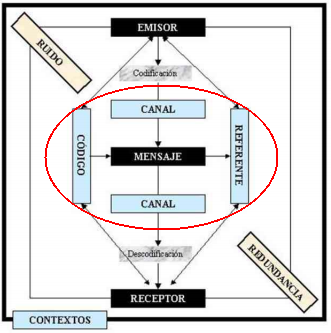
\includegraphics[scale=0.6]{Diseno/comunciacion_modif}}

\caption{Diagrama de comunicación}
\label{comunicacion}
\end{figure}


Estos mecanismos de comunicación por videoconferencia comenzaron a
ser una herramienta esencial para el correcto desarrollo empresarial,
ya que el aprendizaje y comunicación entre sedes alejadas territorialmente,
ya sea de la misma empresa o de empresas del mismo sector, son sin
duda fundamentales para el desarrollo ágil y la búsqueda de soluciones\@.

\smallskip{}


El único inconveniente es el periodo de adaptación desde que se pone
al alcance del ciudadano de a pie una nueva tecnología y el momento
en el cual es utilizada de forma innata hasta llegar a originar una
revolución\@. El avance de la tecnología siempre ha estado ligado
al avance de los interfaces de usuario\@. Una herramienta útil, pero
poco amigable y difícil de utilizar seguramente caerá en desuso\@.
Por este motivo, adaptar las nuevas tecnologías al ser humano es una
guerra en la que aún se lucha por ganar\@. Para este proyecto se
ha jugado con la idea de acercar una sala de videoconferencia al propio
escritorio de cada usuario\@. Se ha intentado mantener la idea de
puerta de entrada y se ha multiplicado el significado de la palabra
llave para dicha puerta\@.

\smallskip{}


Para llevar a cabo la puesta en servicio del proyecto se ha contando
con un escenario inmejorable, el Campus de Excelencia ``Campus do
Mar'' de Vigo\@. En este ámbito nos encontramos con colaboraciones
entre universidades situadas en diferentes comunidades autónomas\@.
Multitud de universidades españolas están trabajando en la actualidad
para obtener una aplicación que agilice, gestione y cuantifique la
reserva de salas virtuales, como es el caso de la aplicación ``Mr.
Bosy'' en la Universidad Carlos III de Madrid\@. Le ofrecemos el
siguiente enlace para acceder al contenido público disponible para
esta aplicación: \href{https://mrbosy.uc3m.es/}{https://mrbosy.uc3m.es/}\@.

\smallskip{}


El diseño visual de este proyecto toma prestada la estética de ``Campus
do Mar'' para facilitar la comprensión al lector de las funciones
realizadas, ya que ha sido el primer lugar donde se ha desplegado
esta aplicación\@. Por el mismo motivo, se ha dotado a la aplicación
con el nombre eMeeting\footnote{Por comodidad nos referiremos a la aplicación con este término a lo largo de la memoria.},
que resulta atractivo al usuario y provee a la aplicación de un arma
más para ser utilizada\@.

\medskip{}



\section{Objetivos\label{sec:Objetivos}}

El presente proyecto surge de la necesidad de una plataforma de videoconferencia
que se adapte a las necesidades y perfiles de usuarios de organizaciones
concretas y facilite el uso de herramientas de videoconferencia a
usuarios que no posean un perfil técnico\@.

\smallskip{}


Todo \textit{software} de videoconferencia intenta brindar el mayor
número de funcionalidades para copar el mercado y conseguir una gran
cartera de clientes, por contrapartida, este hecho conlleva a una
saturación del interfaz de usuario, lo cual dificulta su utilización
en casos concretos\@. Alcanzar una alta proyección y ofrecer un buen
servicio son algunos de los objetivos que se pretenden alcanzar con
este proyecto\@. Aunque una de las más importantes metas ha sido
diseñar una estructura de aplicación que permita adaptar o crear nuevas
funcionaliadades para los constantes cambios de los clientes potenciales
para esta aplicación\@. Esta es una de las principales razones que
nos llevan a desarrollar este proyecto\@.

\smallskip{}


Entre las funcionalidades ma\'{s} destacadas que implementaremos podemos
resaltar la reserva de salas, múltiples posibilidades de disposición
de los elementos de la sala, es decir, se podrá seleccionar el lugar
dónde aparecerán los ponentes en la reunión y el contenido visual
que aporten, también el acceso a gráficas estadísticas que muestran
en tiempo real el uso de la aplicación o un servicio de alerta que
advierte a los administradores de una posible saturación del sistema,
ya sea por exceso de usuarios o por escasez de salas\@.

\smallskip{}


La búsqueda de una aplicación popular tan ansiada por todo desarrollador
web nos obligará a desarrollar un interfaz intuitivo, de forma que
alcancemos una rápida integración de los usuarios sin
necesidad de conocimientos técnicos o lecturas extensas\@.

\smallskip{}


Este proyecto forma parte de un proyecto mayor en el que diferentes
aplicaciones formarán parte de una macroaplicación que dará servicio
al mencionado ``Campus do Mar''\@. Por este motivo, cada aplicación
que forme parte del proyecto debe incluir un servicio que sincronice
las bases de datos de las diferentes aplicaciones que engloba el ``Campus
do Mar'' como pueden ser un calendario o un gestor de tareas, de
manera que todas las aplicaciones formen parte de la macroaplicación
y se comuniquen entre sí\@. Este servicio consigue que la aplicación
sea más completa, incluyendo la opción de integración de una forma
sencilla\@.

\medskip{}



\section{Organización}

Después de esta breve introducción comenzaremos con un capítulo que
sumergirá al lector en el mundo de las tecnologías que se han empleado
para alcanzar los objetivos del proyecto\@. Se hablará de los motivos
que nos han llevado a utilizar unas en detrimento de otras, siempre
siguiendo un criterio de eficiencia temporal, desarrollo ágil, modularidad
y apoyo por parte de la comunidad libre\@.

\smallskip{}


Continuaremos con una descripción del diseño de la aplicación,
construyendo el camino fielmente, desde el primer boceto del interfaz
a los complejos entramados de la base de datos, incluyendo gráficas
ilustrativas que aportarán luz sobre la enmarañada relación interna
de las entidades del proyecto\@. Incluiremos capturas del interfaz
de usuario con el estilo diseñado para el despliegue en ``Campus
do Mar''\@. El departamento de tecnologías de la información y plataforma
digital de ``Campus do Mar'' posee gran cantidad de recursos y por
ello se han llevado a cabo importantes desarrollos tecnológicos en
los que se encuentra integrado este proyecto\@. La importancia de
este departamento es tal que posee nombre propio: ``DigiMar'' y
que se utilizará como referencia a lo largo de este proyecto\@.

\smallskip{}


Se describirán las posibles líneas futuras desprendidas del desarrollo
de la aplicación y de las experiencias de los usuarios que la han
utilizado en la senda del desarrollo eficiente\@. Se comentarán las
ideas que han nacido durante el desarrollo y que han aportado grandes dosis
de conocimiento e intuición para ampliar algunas de las funciones
de la aplicación\@.

\smallskip{}


Se finalizará con la bibliografía empleada en el desarrollo del proyecto
y de esta memoria para el deleite de usuarios con predilección
por el mundo del desarrollo web y sientan el deseo de aumentar sus
conocimientos en este ámbito\@.


\chapter{Tecnologías empleadas\label{chap:Tecnolog=0000EDas-empleadas}}

Toda aplicación web y el trabajo de los desarrolladores tienen unas
premisas comunes, tales como facilitar la interacción usuario-\emph{software}
y, sacando el mayor partido a las tecnologías disponibles, conseguir
resultados adecuados en el menor tiempo posible\@. Para este fin
utilizaremos como motor de videoconferencia el \emph{software} propietario
\textit{Adobe Connect}\textsuperscript{\textregistered{}} y su API,
como motor de administración de bases de datos hemos optado por MySQL,
para el desarrollo de la aplicación nos hemos declinado por el uso
del \textit{framework} Symfony específico para PHP, para las partes
dinámicas que se ejecutan en el explorador hemos decidido utilizar
Javascript y su API jQuery y jQuery UI, para la estructura que se
visualiza en el explorador HTML 5 y para el estilo CSS 3\@. Todas
estas tecnologías a excepción de \textit{Adobe Connect}\textsuperscript{\textregistered{}},
poseen licencia libre, lo cual ayuda al programador en el desarrollo
y la búsqueda de soluciones\@.

\medskip{}



\section{\textit{Adobe Connect}\textsuperscript{\textregistered{}} Profesional}

Ahora más que nunca, la gente necesita la capacidad de colaborar de
forma eficiente con colegas, socios y clientes en todo el mundo, a
través de dispositivos conectados a la red\@. Más y más organizaciones,
incluyendo grandes empresas y agencias del gobierno, están utilizando
\textit{Adobe Connect}\textsuperscript{\textregistered{}}\textsuperscript{}
para conducir extremo a extremo, flujos de trabajo críticos para sus
negocios, reuniones web, \textit{e-Learning} y seminarios. \textit{Adobe Connect}\textsuperscript{\textregistered{}}\textsuperscript{}
ofrece interacciones excepcionalmente ricas y permite a las organizaciones,
desde el Departamento de Defensa de EE.UU. a las corporaciones líderes,
incluyendo Toshiba America o Teltek Vídeo Research, S.L., mejorar
sustancialmente su productividad\@.

\smallskip{}


El \emph{software} propietario \textit{Adobe Connect}\textsuperscript{\textregistered{}}\textsuperscript{}
posee las características más avanzadas de videoconferencia, ofreciendo
un interfaz perfecto para los diferentes tipos de comunicación, ya
sea a nivel académico o profesional\@.

\smallskip{}


El sistema de comunicaciones web \textit{Adobe Connect}\textsuperscript{\textregistered{}}\textsuperscript{}
está compuesto por \textit{Adobe Connect Enterprise Server}\textsuperscript{\textregistered{}}\textsuperscript{}
(versión con licencia) o \textit{Adobe Connect Enterprise Hosted}\textsuperscript{\textregistered{}}\textsuperscript{}
(servicio alojado) y tres módulos, \textit{Adobe Connect Training}\textsuperscript{\textregistered{}}\textsuperscript{},
\textit{Adobe Connect Events}\textsuperscript{\textregistered{}}\textsuperscript{}
y \textit{Adobe Presenter}, que brindan apoyo a las funciones de
\textit{Adobe Acrobat Connect Professional} y las amplían para proporcionar
soluciones de comunicaciones web de formación, \textit{marketing}
y ventas\@. Este \textit{software} propietario es sin duda uno de
los más avanzados del mercado y su completa API nos proporciona la
posibilidad de crear aplicaciones web de gran calidad aprovechando
las características que más convengan a los usuarios finales\@.

\smallskip{}


\textit{Adobe Connect}\textsuperscript{\textregistered{}}\textsuperscript{}
permite a los invitados asistir a sus reuniones fácilmente desde el
escritorio sin necesidad de un cliente de descarga, aunque para este
caso se accederá a través del explorador, y ofrece un completo interfaz
entre dispositivos móviles para incrementar las capacidades de colaboración
y hacer frente a las realidades de los actuales entornos empresariales,
donde los empleados y los clientes están en continuo movimiento\@.
Este complejo entramado en que se ha convertido la vida laboral e
incluso privada de las personas, de la mano de las nuevas tecnologías
de la comunicación y la información, hace indispensable la utilización
de \textit{software} de estas características, donde uno de los factores
más importantes es el ahorro de tiempo y dinero\@. En un mundo sustancialmente
capitalista como el actual, son dos pilares básicos para la sostenibilidad
del sistema y como no podía ser de otro modo, en tiempos de crisis
cualquier ventaja puede ser la diferencia entre el éxito y el fracaso\@.

\smallskip{}


La experiencia del usuario ha desvelado que el uso de \textit{Adobe Connect Profesional}\textsuperscript{\textregistered{}}\textsuperscript{}
es complejo para cualquier usuario que no posea un perfil técnico
y carece de las necesidades específicas de los usuarios de ``Campus
do Mar'', este hecho provoca el nacimiento de esta aplicación\@.

\medskip{}



\section{SYMFONY\label{sec:SYMFONY}}

En las siguientes líneas abordaremos la solución a un problema mediante
un \textit{framework} específico para PHP y destinado al desarrollo
de aplicaciones web\@. Una gran lista de aplicaciones se han desarrollado
bajo el \textit{framework} Symfony como Motilee (para crear foros
de discusión), SteerCMS (gestor de contenidos), Hashbin (facilita
la depuración colaborativa de las aplicaciones), Symfonians (punto
de encuentro de usuarios y desarrolladores de Symfony), LiveChat (añadir
a un sitio web chats en tiempo real), Lichess (servidor de juegos
de ajedrez) \cite{key-7}\@.

\smallskip{}


Symfony es un \textit{framework} PHP que facilita la organización
y el desarrollo de las aplicaciones web, es decir, se encarga de todos
los aspectos comunes y aburridos, dejando que el programador se dedique
a aportar valor, desarrollando las características únicas de cada
proyecto\@. En este proyecto se ha utilizado la segunda versión de
este \textit{framework} que posee una importante cantidad de mejoras
tanto a nivel de desarrollador como internas, cabe resaltar el aumento
de la compatibilidad con versiones futuras, mucho menos trabajado
en el pasado\@. Es por ello que las referencias a Symfony pertencen
en todo el proyecto a su segunda versión, por tanto tendremos partes
comunes y mejoras con respecto a versiones anteriores\@.

\smallskip{}


Típicamente, puede incluir soporte de programas, bibliotecas, y un
lenguaje interpretado, entre otras herramientas, para así ayudar a
desarrollar y unir los diferentes componentes de un proyecto\@. Representa
una arquitectura de \emph{software} que modela las relaciones generales
de las entidades del dominio, y provee una estructura y una especial
metodología de trabajo, la cual extiende a las aplicaciones del dominio\@.
Las principales herramientas de Symfony imprescindibles para este
proyecto se describen a continuación\@.

\medskip{}



\subsection{El controlador}

En esta sección se mostrará cómo se organizan y qué son los controladores
en la estructura de Symfony\@.

\smallskip{}


Se llama controlador al conjunto de directorios, en este proyecto situados
en la carpeta \textit{src/Cmar/MeetingBundle}, que almacenan la lógica
de los diferentes elementos de la aplicación\@. Es, por así
decirlo, el cerebro de cada una de las funciones que se realizan\@.
El controlador recoge los datos de los formularios y de la base de
datos y ofrece las respuestas que se visualizarán en las plantillas
Twig, que describiremos en la sección \ref{sub:La-vista}\@.

\smallskip{}


Ofrecen la posibilidad de generar respuestas, como páginas HTML
o ficheros XML para fuentes RSS o servicios Web, y JSON para peticiones
AJAX, ajustando únicamente el valor de la variable \textit{format}
en la descripción de las funciones del controlador para las cuales
se necesite un tipo de respuesta u otra\@. Posee instrucciones específicas
para acce\-der al objeto \textit{request}\footnote{Se utiliza nomenclatura PHP para esta variable.},
o de respuesta de un formulario, a través de una variable llamada
\textit{app.request}\cite{key-7}\cite{key-3}\@.

\smallskip{}


Symfony posee un elegante objeto de sesión que representa el cliente
(puede ser una persona real usando un navegador, un \textit{bot}
o un servicio web)\@. Entre dos peticiones, Symfony almacena los
atributos en una cookie usando sesiones nativas de PHP\@. De esta
forma es posible generar funciones del tipo migas de pan de forma sencilla
utilizando los atributos de esta \textit{cookie} o generar acceso
a un servidor evitando peticiones superfluas si aún no ha caducado
la sesión\@.

\medskip{}



\subsection{Arquitectura\label{sub:Arquitectura}}

Uno de los principales beneficios de la utilización de un \textit{framework}
completo es normalizar los desarrollos\@. Gracias a la estructura
predeterminada de archivos y directorios de Symfony, cualquier desarrollador
con conocimientos básicos puede asumir el mantenimiento de un proyecto
elaborado con este \textit{framework}, premisa muy importante para
el desarrollo colaborativo de cualquier aplicación\@.

\smallskip{}


Se adjunta una breve descripción de la funcionalidad de cada directorio
de Symfony en la figura \ref{Explic-direct-Symfony}\@.

\smallskip{}


\begin{figure}[H]
\centerline{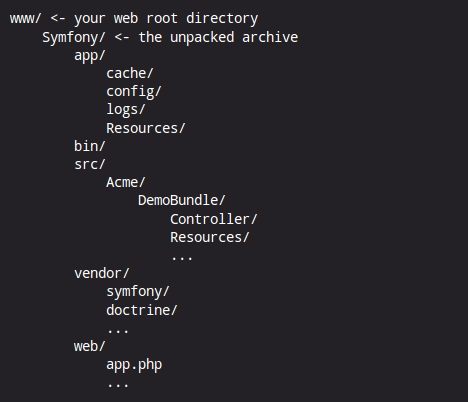
\includegraphics[scale=0.5]{EstructuraDirectoriosSymfony}}

\caption{Estrucutra de directorios en Symfony}
\label{estruc-direct-Sym}
\end{figure}


\begin{figure}
\centerline{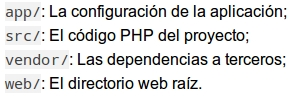
\includegraphics[scale=0.5]{ExplicacionEstructuraDirectoriosSymfony}}

\caption{Funcionalidades de la estucutra de directorios en Symfony}
\label{Explic-direct-Symfony}
\end{figure}

\begin{itemize}
\item \colorbox{lightgray}{web/}: El directorio web raíz es el hogar de
todos los archivo públicos y estáticos como imágenes, hojas de estilo
y archivos JavaScript. También reside cada controlador frontal\@.
Un pequeño script PHP cuyo trabajo es arrancar la aplicación\@. El
\textit{kernel} requiere primero del archivo bootstrap.php, el cual inicia
el \textit{framework} y registra al \textit{autoloader}\@. Como
cualquier controlador frontal, \textit{app.php} usa una clase \textit{Kernel},
llamada \textit{AppKernel}, para iniciar la aplicación\@.
\item \colorbox{lightgray}{app/}: La clase \textit{AppKernel} es el punto
de ingreso principal a la configuración de la aplicación y como tal,
se ubica en este directorio\@.

\begin{itemize}
\item La velocidad de Symfony se debe a su sistema de caché\@. La configuración
de la aplicación sólo es analizada durante el primer \textit{request}
y luego compilada a código PHP que se guarda en el directorio \textit{app/cache/}\@.
\item Durante el desarrollo de una aplicación web, las cosas pueden salir
mal de muchas maneras. Los archivos de log en el directorio \textit{app/logs/}
de la aplicación ofrecen todo lo necesario sobre los \textit{requests} para
arreglar el problema rápidamente\@.
\end{itemize}
\item \colorbox{lightgray}{vendor/}: Las librerías de terceros deberían
estar ubicadas en este directorio que contiene inicialmente las bibliotecas
de Symfony, SwiftMailer, el ORM Doctrine, el sistema de plantillas
Twig y una selección de clases de \textit{Zend Framework}, pero esto
es sólo una convención siendo posible ubicarse en un directorio global
del servidor o en uno local en cada proyecto\@.
\item \colorbox{lightgray}{src/}: Para describir este directorio es impresdindible
mencionar el sistema de \textit{bundles}, una de las más grandiosas
y poderosas características de Symfony\@. Un \textit{bundle} es
similar a un \textit{plugin} en otros lenguajes\@. Recibe el nombre
de \textit{bundle} y no de \textit{plugin} porque \textit{todo}
es un \textit{bundle} en Symfony\@. Esto le da la flexibilidad de
usar características pre-construidas empaquetadas en \textit{bundles}
de terceros o distribuir sus propios \textit{bundles}\@. Cada \textit{bundle}
puede ser adaptado por medio de archivos de configuración escritos
en YAML, XML o PHP\@. Cada entrada llamada \textit{framework} en
el archivo de configuración define la composición para un \textit{bundle}\@.
Y a su vez cada entorno dentro del directorio \textit{src/} puede
sobreescribir la configuración por omisión si se provee de un archivo
de configuración específico \cite{key-18}\@. Además de ser una buena
manera de organizar y configurar el código, un \textit{bundle} puede
extender otro, ya que los \textit{bundles} soportan herencia\@.
Esto le permite sobreescribir un \textit{bundle} existente para adaptar
sus controladores, plantillas y cualquier archivo que contenga\@.
Es aquí donde los nombres lógicos resultan útiles ya que abstraen
al programador del lugar en donde se encuentra realmente ubicado el
recurso\@. Por este motivo como se verá en el apartado de diseño,
los controladores tendrán nombres que hacen referencia a la función
que desempeñan\@. A su vez Symfony crea una estructura de directorios
por cada aplicación que se define con el comando Symfony \textit{generate:app}\@.
\end{itemize}
\smallskip{}


La estructura de directorios de la aplicación eMeeting parte de la base
estructural de Symfony que se describe en la figura \ref{estruc-direct-Sym}\@.
A esta base estructural se le añade, en sus correspondientes directorios,
los componentes que la aplicación necesita, de forma que se obtiene
una estructura de directorios como la que se muestra en la figura
\ref{estruc-direct-eMeeting}\@.

\smallskip{}


\begin{wrapfigure}{L}{0.28\columnwidth}%
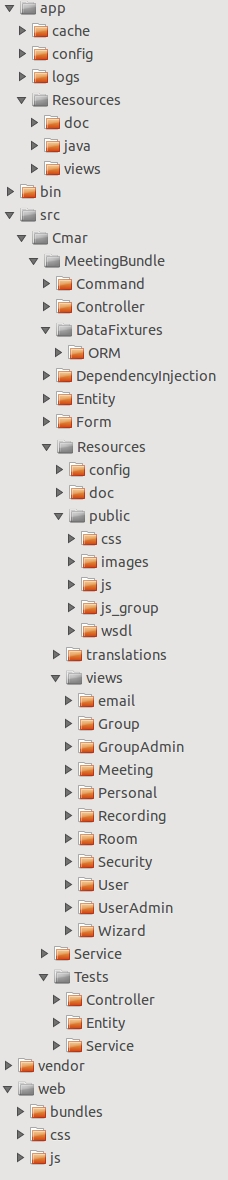
\includegraphics[scale=0.4]{Lista_directorios_eMeeting}

\caption{Estructura de directorios de eMee\-ting}
\label{estruc-direct-eMeeting}\end{wrapfigure}%


El contenido y la razón de la existencia de los directorios específicos
para la aplicación serán descritos con detalle en el capítulo
\ref{chap:Dise=0000F1o-del-proyecto}\@.

\medskip{}



\subsection{La vista\label{sub:La-vista}}
\begin{itemize}
\item La plantilla TWIG


Twig es el motor de plantillas para PHP que utiliza Symfony\@. Sus
características principales son:
\begin{itemize}
\item Rápido: Ofrece la posibilidad de optimizar las llamadas a los contenidos
de las variables que PHP envía a las plantillas HTML\@. El tiempo
de generación de las plantillas, en comparación con el habitual código
PHP, se ve reducido a la mínima expresión\@.
\item Seguro: Tiene un modo para evaluar código en la plantilla que no es
de confianza. Esto permite utilizarlo como un lenguaje de plantillas
para aplicaciones en las que los usuarios pueden modificar el diseño
de la plantilla\@. El objetivo de modularidad de eMeeting
agradece enormemente el uso de este motor de plantillas\@.
\item Flexible: Posee un analizador léxico flexible. Esto permite al desarrollador
definir sus propias etiquetas y filtros personalizados, y crear su
propio lenguaje específico del dominio (DSL) \cite{key-17}\@.
\end{itemize}

\smallskip{}



Todas las plantillas utilizadas por la aplicación eMeeting se han
realizado con este formato, optimizando la compilación y facilitando
el acceso a los contenidos de las variables de la base de datos utilizadas
en la lógica implementada con PHP\@.


\smallskip{}



Permite una sencilla herencia de plantillas
para evitar la redundancia de código o incluir URIs que hacen referencia
a páginas del propio código de la aplicación\@. Las plantillas para cada sección
de eMeeting se alojan en la carpeta \textit{src/Cmar/MeetingBundle/views}\@.

\end{itemize}
\medskip{}



\subsection{Doctrine}

El proyecto Doctrine consta de un conjunto de bibliotecas PHP seleccionadas
principalmente para ofrecer servicios de persistencia y funcionalidades
en las relaciones sobre las bases de datos utilizadas\@. Entre
sus principales características cabe destacar el asignador relacional
de objetos (ORM) y la capa de abstracción de base de datos\@.

\smallskip{}


Esta herramienta de Symfony permite actuar sobre la base de datos
de una forma sencilla y en cualquier parte del código ya que permite
abstraer al programador del motor de base de datos utilizado\@.
Esta característica permite aumentar la modularidad del
proyecto y poder desplegarlo sobre el motor de base de datos que posea
el usuario final sin modificar apenas líneas de código\@. Sin duda,
alguna de las consultas específicas y complejas que realice la
aplicación deberán ser reescritas para adaptarse al nuevo entorno,
pero se intentará que sean ínfimas para cumplir con la modularidad
propuesta en los objetivos del proyecto \cite{key-7}\@.

\medskip{}



\subsubsection{Asignador Relacional de Objetos}

El asignador relacional de objetos (ORM) para PHP se encuentra en
la parte superior de una poderosa abstracción en la capa de la base
de datos (DBAL)\@. Una de sus principales características es la opción
de escribir las consultas de bases de datos en un dialecto propio
orientado a objetos llamado Lenguaje SQL de consulta de Doctrine (DQL),
inspirado en Hiberna HQL\@. Esto proporciona a los desarrolladores
una poderosa alternativa a SQL que mantiene la flexibilidad sin necesidad
de duplicar el código innecesariamente \cite{key-7}\@.

\medskip{}



\subsubsection{Capa de abstracción de la base de datos}

Posee múltiples características para la introspección en el esquema
de la base de datos, la administración de esquemas y la abstracción
PDO\@.

\smallskip{}


La abstracción de base de datos de Doctrine y la capa de acceso (DBAL)
ofrece una capa ligera alrededor de un API de PDO-like y multitud
de características adicionales, como la introspección horizontal en
el esquema de la base de datos y la manipulación a través de una API
orientada a objetos\@.

El hecho de que la DBAL de Doctrine abstrae del pesado API DOP mediante
el uso de interfaces que se parecen mucho a la actual API de PDO,
hace posible la implementación de los controladores personalizados
que pueden utilizar las API's nativas existentes o las realizadas
por el propio programador \cite{key-7}\@.

\smallskip{}


Para optimizar y aprovechar al máximo el uso de Doctrine se deben
describir las tablas de la base de datos con el formato específico
adoptado por Symfony en sus desarrollos para el ORM llamado \textit{YAML},
que se describe a continuación\@.

\medskip{}



\subsection{El Formato YAML}

De acuerdo con el sitio web oficial YAML ``es una serialización de
datos estándar muy amigable para todos los lenguajes de programación''\@.
Dicho de otra manera, YAML es un lenguaje sencillo para describir
los datos (\emph{strings, integers, dates, arrays y hashes}).

\smallskip{}


En YAML, la estructura se muestra a través de la sangría, la secuencia
de elementos se denotan por un guión, y los pares clave/valor están
separados por dos puntos\@. YAML también tiene una sintaxis abreviada
para des\-cribir la misma estructura con menos líneas, donde los arrays
explícitamente se muestran con {[}{]} y los hashes o array asociativos
con \{\} \cite{key-9}\@.

\smallskip{}


El \textit{framework} Symfony lo utiliza ampliamente para sus archivos de configuración
o para la creación de tablas y estructuras de Doctrine\@. Por ejemplo
en los ficheros \textit{security.yml} y \textit{routing.yml} que
se mencionarán en la sección \ref{sec:Seguridad-de-la}\@. Estos ficheros
siguen la estructura típica de un fichero YAML y la relación entre
ambos ofrece la seguridad para cada ruta de la aplicación\@. Como
se verá en el capítulo \ref{chap:Desarrollo-del-proyecto}, las rutas
de Symfony cobran especial importancia ya que están asociadas a funciones,
en caso de que sea necesario, y la seguridad de algunas de estas funciones puede
ser crítica\@.

\smallskip{}


Gracias al archivo de descripción de la base de datos \textit{schema.yml},
es posible utilizar más ampliamente las simplificaciones que ofrece Doctrine
al generar los comandos SQL necesarios para crear las tablas en la
base de datos\@. 

\smallskip{}


Se describe, a modo de ejemplo, alguna de estas tareas:
\begin{itemize}
\item Para generar el SQL se debe construir el modelo a partir del contenido
del archivo \textit{schema.yml}\@.


\begin{lstlisting}
php symfony doctrine:build-model
\end{lstlisting}

\item Ahora que los modelos existen se puede generar e insertar el SQL.


\begin{lstlisting}
php symfony doctrine:build-sql
\end{lstlisting}

\item La tarea doctrine:build-sql genera comandos SQL en el directorio \textit{data/sql/},
optimizado para el motor de base de datos que se ha configurado, en
el caso de eMeeting MySQL\@.
\end{itemize}
\smallskip{}


Gracias a esta característica, cualquier cambio en la base de datos,
como añadir un nuevo campo a una entidad, lo que equivale a una nueva
columna en la tabla correspondiente, con su valor es una acción simple
y que Doctrine realizará de forma limpia y sin hacer peligrar el contenido
de la base de datos\@. Ofrece funcionalidades como visualizar qué
comandos específicos para la base de datos se realizarán con el cambio
implementado, evitando así pérdidas de datos o acciones que traerán
consecuencias irreversibles\@.

\medskip{}



\subsection{Las entidades}

Estos elementos de Symfony guardan la estructura de las piezas del
juego de la aplicación\@. A partir de la estructura de las entidades,
Doctrine construirá los elementos que rellenarán las tablas de la
base de datos y aportarán las características y relaciones que se insertarán
en las cabeceras de estos elementos\@.

\smallskip{}


Las entidades aportan al proyecto una gran modularidad ya que
se podrá insertar un nuevo elemento en la base de datos o un
nuevo campo en el elemento preciso para incrementar las funcionalidades
o complementar las existentes si se queda en el tintero alguna que
se descubra en el proceso de puesta en servicio\@. También ofrece
facilidades a la hora de corregir errores en el proceso de diseño
o cuando la aplicación está ya en producción\@. 

\medskip{}



\section{PHP}

PHP tal y como se conoce hoy en día es en realidad el sucesor de un
producto llamado PHP/FI. Creado en 1994 por Rasmus Lerdorf\@.

\smallskip{}


La primera encarnación de PHP era un conjunto simple de ficheros binarios
\textit{Common Gateway Interface} (CGI) escritos en el lenguaje de
programación C. Originalmente utilizado para rastrear visitas de su
currículum online, llamó al conjunto de \textit{scripts} ``\textit{Personal Home Page Tools}'',
más frecuentemente referenciado como ``\textit{PHP Tools}''\@.

\smallskip{}


En junio de 1995, Rasmus publicó el codigo fuente de \textit{PHP Tools},
lo que permitió a los desarrolladores usarlo como considerasen apropiado\@.
Esto animó a los usuarios y permitió que proporcionasen soluciones
a los errores del código \cite{key-10}\@.

\smallskip{}


\begin{figure}
\centerline{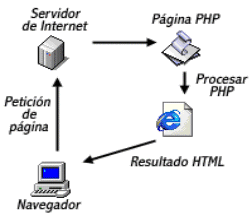
\includegraphics[scale=0.6]{Diseno/PHP_arq}}

\caption{Procesos que describen PHP}
\end{figure}


Es un lenguaje interpretado orientado al desarrollo de aplicaciones
web dinámicas con acceso a información almacenada en una base de datos\@.
El código fuente escrito en PHP es invisible al navegador web y al
cliente ya que es el servidor el que se encarga de ejecutar el código
y enviar su resultado HTML al navegador\@. Esto hace que la programación
en PHP sea segura y confiable\@. Aunque puede ser usado también desde
un interfaz de línea de comandos o como aplicación de escritorio\@.
Implementa capacidad de conexión con la mayoría de los motores de
base de datos que se utilizan en la actualidad, destaca su conectividad
con MySQL y PostgreSQL\@. Posee la capacidad de expandir su potencial
utilizando módulos\@. Permite aplicar técnicas de programación orientada
a objetos\@. No requiere definición de tipos de variables aunque
sus variables se pueden evaluar también por el tipo que estén manejando
en tiempo de ejecución\@. PHP5 incorpora manejo de excepciones, una
gran herramienta para el desarrollo de aplicaciones complejas orientadas
a la interacción con usuarios, tales como aplicaciones web\@.

\smallskip{}


Si bien PHP no obliga a quien lo usa a seguir una determinada metodología
a la hora de programar, el programador puede aplicar en su trabajo
cualquier técnica de programación o de desarrollo que le permita escribir
código ordenado, estructurado y manejable. Un ejemplo de esto son
los desarrollos que en PHP se han hecho del patrón de diseño Modelo
Vista Controlador (MVC), que permiten separar el tratamiento y acceso
a los datos, la lógica de control y la interfaz de usuario en tres
componentes independientes\@.

\medskip{}



\section{Apache}

Como servidor web de la aplicación se ha optado por la opción
de Apache 2\@. Utilizando PHP para el desarrollo es obvio el uso
de Apache ya que existe un módulo específico de forma que se aprovecha
al máximo la integración con el servidor y se alcanzan velocidades excelentes\@.

\smallskip{}


El servidor HTTP Apache es un servidor web libre y de código abierto,
el más popular en cuanto a uso, sirviendo de facto como plataforma
de referencia para el diseño y evaluación de otros servidores web\@.
Pero en la actualidad está incrementando su utilización para uso comercial\@.

\begin{wrapfigure}{L}{0.4\columnwidth}%
\centerline{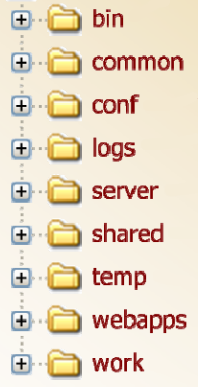
\includegraphics[scale=0.5]{Diseno/apache_estruc}}

\caption{Arquitectura de directorios de Apache}


\label{Apache_estruct}\end{wrapfigure}%


Los directorios de Apache albergan funciones de muy diferentes tipos
como configuración, almacenamiento de librerías, etc\@. Se dispone
a continuación un breve recorrido por la estructura reflejada
en la figura \ref{Apache_estruct}, que aclarará algunos conceptos
sobre este servidor web\@.

\smallskip{}


En el directorio \textit{bin/} se encuentra el ejecutable para arrancar
la aplicación, diferentes \textit{scripts} y el precompilador de
JSP\@. En \textit{common/} se albergan clases y JARs accesibles
a todas las aplicaciones web y al propio Apache\@. Los archivos de
configuración, como por ejemplo el \textit{server.xml}, se encuentran
en \textit{conf/}\@. Los archivos de registro y los elementos de
consulta de posibles errores en las aplicaciones se albergan en el
directorio \textit{logs/}\@. El directorio \textit{server/} ha
sido creado para albergar clases y aplicaciones sólo accesibles por
Apache\@. Las clases y JARs accesibles por todas las aplicaciones
web se almacenan en \textit{shared/}\@. Como era de esperar los
archivos temporales que genera Apache se alamcenan en \textit{temp/}\@.
Las aplicaciones web de ejemplo, las creadas por usuarios y otras
propias de Apache se almacenen en \textit{webapps/}\@. En este directorio
se encuentran los archivos WAR (\textit{Web Application Archive}
- Archivo de aplicación web), que son archivos JAR utilizados para
distribuir una colección de \textit{JavaServer Pages}, \textit{servlets},
clases Java, archivos XML, librerías de \textit{tags} y páginas web
estáticas (HTML y archivos relacionados) que juntos constituyen una
aplicación web\@. Y por último, en el directorio \textit{work/}
se almacenan archivos temporales, como los JSP compilados, etc\@.

\smallskip{}


Algunas entornos de desarrollo como Eclipse o NetBeans instalan su
propia instancia de Apache utilizando su propia configuración, lo
que evita tener que instalar \textit{plugins} para integrar Apache
y generar archivos WAR para distribuir la aplicación web fácilmente
u otros menesteres\@.

\smallskip{}


En el interior del directorio \textit{webapps/} se encuentra la raíz
de la aplicación web, aunque para el caso que nos atañe se ha modificado el archivo
\textit{default} en el interior del servidor creando un \textit{virtualhost}
que redirecciona la petición sobre una URL determinada, que para el 
caso de eMeeting será \textit{emeeting.campusdomar.es, emeetings.campusdomar.es, mee\-ting.campusdomar.es, meetings.cam\-pusdomar.es}, a la carpeta \textit{web} de Symfony donde se
encuentra el fichero \textit{app.php} que arranca la aplicación\@.

\smallskip{}


También existen los directorios \textit{WEB-INF} y \textit{META-INF}
(opcional), situados en una zona privada de la aplicación\@. \textit{WEB-INF}
contiene el descriptor de despliegue de la aplicación, las clases
compiladas, las bibliotecas de clases y las etiquetas para usar en
los documentos JSP\@. \textit{META-INF} suele contener sólo el archivo
\textit{MANIFEST.MF}, que indica las bibliotecas de las que depende
la aplicación\@. Se suele generar automáticamente\@.

\medskip{}



\section{Javascript}

JavaScript es un lenguaje de programación que se utiliza principalmente
para crear páginas web dinámicas\@.

\smallskip{}


Una página web dinámica es aquella que incorpora efectos como texto
que aparece y desaparece, animaciones, acciones que se activan al
pulsar botones y ventanas con mensajes de aviso al usuario\@.

\smallskip{}


En esta sección se hablará de las librerías javascript utilizadas para
realizar las animaciones del interfaz de usuario, la implementación
de peticiones AJAX y la lógica en la que se apoyan algunas de las
funciones Javascript propias que se describirán en la subsección \ref{sub:Funciones-propias}\@.

\smallskip{}


Técnicamente, JavaScript es un lenguaje de programación interpretado,
por lo que no es necesario compilar los programas para ejecutarlos.
En otras palabras, los programas escritos con JavaScript se pueden
probar directamente en cualquier navegador sin necesidad de procesos
intermedios\@.

\smallskip{}


A pesar de su nombre, JavaScript no guarda ninguna relación directa
con el lenguaje de programación Java\@.

\medskip{}



\subsection{jQuery}

jQuery es una librería de JavaScript rápida y concisa que simplifica
el código en do\-cumentos HTML, manejo de eventos, animación, y las
interacciones Ajax para el desarrollo web rápido\@.

\smallskip{}


El proyecto jQuery comenzó como una idea en 2005 y ha crecido hasta
convertirse en el conjunto de proyectos que conocemos hoy en día.
jQuery está diseñado para cambiar la forma en que el usuario escribe
JavaScript. Sin duda utilizar la API de cualquier \emph{software}
es cómodo y sencillo\@. Es un camino rápido para conseguir funcionalidades
en una aplicación o página web, de una forma rápida obteniendo unos
resultados verdaderamente satisfactorios \cite{key-12}\@.

\smallskip{}

\begin{itemize}
\item jQuery 1.7.1


En esta subsección se hablará de las mejoras que incorpora esta versión
con respecto a sus predecesoras\@.


Una de las mejoras es la unificación de todos los caminos para lanzar
eventos y dete\-nerlos en un documento jQuery en las APIs \textit{.on()}
y \textit{off()\@.}


\begin{lstlisting}
$(elements).on( events [, selector] [, data], handler(EventObject) ); 

$(elements).off( events [, selector] [, handler(EventObject) ]);
\end{lstlisting}


Esta mejora facilita la programación y evita las confusiones en casos
especiales de objetos que no poseen determinados eventos o donde la
forma de ejecutar un evento debido al tipo de elemento desde el que
precisa lanzar el evento se realiza con la función \textit{.todelegate()}
o \textit{.bind()}\@.


Lanzar eventos se ha convertido en una práctica cada vez más importante
con el crecimiento del tamaño y la complejidad de las páginas\@.
Marcos de aplicaciones como Backbone, JavaScriptMVC y SproutCore hacen
un uso intensivo del lanzamiento de eventos. Con esto en mente, jQuery
1.7 refactoriza el lanzamiento de eventos con miras a lanzar eventos
mucho más rápido, especialmente para los casos más comunes\@.


Para optimizar el código de los casos más utilizados, se analizó una
muestra representativa de código de Google Code Search. Casi dos tercios
de los selectores utilizados en \textit{.life()} y \textit{.todelegate()}
llaman a métodos con la etiqueta \textit{tag\#id.class}\@.\cite{key-13}

\item jQuery-ui-1.8.18


Esta librería es sencilla y fácil de manejar utilizando la documentación
detallada y sus tutoriales, además existe una comunidad muy activa
a disposición de cualquier usuario\@. Compatible con IE 6.0 +, Firefox
3 +, Safari 3.1 +, Opera 9.6 + y Google Chrome\@. Ofrece al usuario
una enorme potencia, que permite alcanzar un alto nivel funcional en toda aplicación
web\@.


jQuery UI proporciona abstracciones de bajo nivel de interacción y
animación, efectos avanzados y de alto nivel y \textit{widgets} configurables\@.
Está construido en la parte superior de la librería jQuery de JavaScript,
y se utiliza para crear aplicaciones web altamente interactivas \cite{key-12}\cite{key-13}\@.

\item jQuery-kamicgraphs


Esta potente librería para generar gráficas es utilizada en este proyecto
para mostrar las estadísticas al administrador\@. Con peticiones
AJAX se seleccionan tablas o entradas en la base de datos y posee un inmenso repertorio
de gráficas para mostrar resultados a partir de los datos en formato
JSON que le sirven las aplicaciones\@.

\item jQuery-tipTip


Esta librería ofrece un amplio repertorio de animaciones para mostrar
datos en ventanas emergentes o flotantes\@.\textit{ TipTip} detecta
los bordes de la ventana del navegador y se asegurará de que la descripción
incluída en las ventanas que genera se queda en el interior de la
ventana actual. Como resultado, la información de una herramienta
se ajusta para aparecer encima, debajo, a la izquierda o a la derecha
del elemento, dependiendo de la necesidad para permanecer dentro de
la ventana del navegador. \textit{TipTip} es muy ligero y personalizable
fácilmente\@. Todos los menús de información para los botones e iconos
de ayuda de eMeeting se implementan con la ventana emergente de información 
que ofrece \textit{TipTip}\@.

\end{itemize}

\section{MySQL}

MySQL es un Sistema de Gestión de Bases de Datos (SGBD) relacional,
que por lo tanto utiliza SQL, multihilo y multiusuario del que se
estiman más de un millón de instalaciones\@.

\smallskip{}


Lo que durante un tiempo se consideró como un sencillo juguete para
su uso en lugares web, se ha convertido en la actualidad en una solución
viable y de misión crítica para la administración de datos\@. Anteriormente,
MySQL se consideraba como la opción ideal para webs principalmente
por su gran velocidad\@. Sin embargo, en la actualidad incorpora
muchas de las funciones necesarias para otros entornos conservando
su rapidez característica\@. MySQL supera desde hace tiempo a muchas
soluciones comerciales en velocidad y dispone de un sistema de permisos
elegante y potente, además, la versión 4 incluye el motor de almacenamiento
InnoDB compatible con ACID\@.

\smallskip{}


Los registros de las tablas InnoDB tienen las siguientes características:

\smallskip{}

\begin{itemize}
\item Cada registro de índice en InnoDB contiene un encabezado de seis bytes\@.
El encabezado se emplea para enlazar entre sí registros consecutivos,
y también en el bloqueo a nivel de fila\@.
\item Los registros en el índice agrupado contienen campos para todas las
columnas definidas por el usuario\@. Adicionalmente, hay un campo
de seis bytes para el identificador de transacción y un campo de siete
bytes para el \textit{roll pointer}\@.
\item Si no se definió una clave primaria para la tabla, cada registro de
índice agrupado contiene un campo de identificación de fila de seis
bytes\@.
\item Cada registro de índice secundario contiene también todos los campos
definidos para la clave del índice agrupado\@.
\item Un registro contiene además un puntero a cada campo del mismo\@.
Si la longitud total de los campos en un registro es menor de 128
bytes, el puntero medirá un byte, de lo contrario, tendrá dos bytes
de longitud\@. La matriz de estos punteros se conoce como el directorio
de registros\@. El área a donde señalan estos punteros se denomina
parte de datos del registro\@.
\item Internamente, InnoDB almacena las columnas de caracteres de longitud
fija en un formato de longitud fija\@. InnoDB trunca los espacios
sobrantes de las columnas VARCHAR\@. Nótese que MySQL puede convertir
internamente columnas CHAR a VARCHAR\@.
\item Un valor NULL SQL reserva 1 ó 2 bytes en el directorio de registros\@.
No reservará ningún byte en la parte de datos del registro si se almacena
en una columna de longitud variable\@. En una columna de longitud
fija, reservará en la parte de datos la longitud asignada a dicha
columna\@. La razón por la que se reserva este espacio fijo a pesar
de tratarse de un valor NULL, es que en el futuro se podrá insertar
en su lugar un valor distinto de NULL sin provocar la fragmentación de la página
de índice\@.
\end{itemize}
\smallskip{}


Los nombres de bases de datos, tablas, índices, columnas y alias son
identificadores\@. Los identificadores de MySQL tienen una sintaxis
concreta\@. La longitud máxima para bases de datos, tablas, índices
y columnas es de 64 bytes y para alias de 255 bytes\@.

\smallskip{}


Adicionalmente a las restricciones que se acaban de detallar, ningún
identificador puede contener un caracter ASCII 0 o un byte con un
valor de 255\@. Los nombres de bases de datos, tablas y columnas
no deberían terminar con caracteres de espacio\@. MySQL 5.0 permite
el uso de comillas en identificadores, aunque es mejor evitarlos tanto
como sea posible\@.

\smallskip{}


Los identificadores se almacenan empleando Unicode (UTF8). Esto se
aplica a identificadores en las definiciones de tabla que se almacenan
en ficheros .frm y a identificadores almacenados en las tablas de
permisos en la base de datos mysql\@.

\smallskip{}


Es preciso ser cuidadoso al utilizar MD5 para producir nombres de
tablas, porque puede producir nombres ilegales\@. En el caso de eMeeting
el MD5 es usado únicamente para generar unas URLs especiales para
el acceso de usuarios y se almacenan en las tablas, pero nunca es
utilizado para generar nombres de tablas\@.

\smallskip{}


MySQL posee procedimientos almacenados y funciones que son funcionalidades
añadidas a partir de la versión de MySQL 5.0\@. Un procedimiento
almacenado es un conjunto de comandos SQL que pueden almacenarse en
el servidor\@. Una vez que se hace, los clientes no necesitan relanzar
los comandos individuales pero pueden en su lugar referirse al proce\-dimiento
almacenado\@.

\smallskip{}


Los procedimientos almacenados pueden mejorar el rendimiento ya que
se necesita enviar menos información entre el servidor y el cliente\@.
Por contra se aumenta la carga de la base de datos del servidor ya
que la mayoría del trabajo se realiza en la parte del servidor y no
en el cliente\@.

\smallskip{}


Los procedimientos almacenados permiten tener bibliotecas o funciones
en el servidor que sirve de base de datos\@. Esta característica
es compartida por los lenguajes de programación modernos que permiten
este diseño interno, por ejemplo, usando clases\@.

\smallskip{}


MySQL sigue la sintaxis SQL:2008 para procedimientos almacenados\@.

\smallskip{}


Muchas de estas restricciones son corregidas por Doctrine y, en caso
de no tener la capacidad de correción, la generación de las estructuras
de la base de datos mediante las instrucciones propias de Doctrine
ofrecerá los errores correspondientes para una rápida corrección del
código erróneo\@.

\medskip{}



\section{HTML 5 y CSS 3}

La elección de este avanzado lenguaje es obvia\@. Dentro de no muchos
años todos los exploradores sorportarán únicamente HTML 5 que incluye
unas mejoras para la visualización de vídeos muy importantes e incluye
características de estilo novedosas, con la ayuda de Twig es altamente
eficiente la creación de plantillas HTML y la última versión revisada
es la mejor opción en la actualidad\@.

\smallskip{}


CSS 3 incluye las últimas mejoras en el diseño de interfaces y en
compatibilidad con exploradores\@. De esta forma se sacará el mayor
partido al diseño y se facilitará la compatibilidad con todos
los exploradores del mercado\@. El consorcio W3C valora cualquier
cambio que se realice para conseguir un estándar actualizado y compatible
con el mayor número de exploradores, por ello las novedades que incorpora
CSS en su tercera versión son altamente recomendables\@.

\chapter{Decisiones de diseño\label{chap:Dise=0000F1o-del-proyecto}}

En este capítulo se ofrecen los diferentes motivos de las decisiones
que se han tomado para el posterior desarrollo del proyecto\@. Las
premisas fundamentales han sido el desarrollo ágil y la obtención
de un resultado óptimo en el menor tiempo posible\@.

\medskip{}



\section{\noindent \textit{Adobe Connect}\textsuperscript{\textregistered{}}\textsuperscript{}\label{sec:AdobeConnectProfessional}}

Durante más de 25 años, \emph{Adobe} ha revolucionado la interacción
de todo el mundo con ideas e información\@. Tanto en la web como
en papel, en vídeo o en dispositivos móviles, las tecnologías y el
\emph{software} de Adobe han llegado a todos los rincones del mundo.
Adobe Flash\textsuperscript{\textregistered{}} Player es la plataforma
de \emph{software} más extendida, y se encuentra instalada en más
del 98 \% de los equipos de escritorio con conexión a Internet\@.
La tecnología Adobe Flash es la más utilizada para producir vídeo
en la Web, mientras que el \emph{software} Adobe Reader\textsuperscript{\textregistered{}}
se ha convertido en el estándar mundial para compartir documentos
e información\@. Las famosas marcas de Adobe como Adobe Photoshop\textsuperscript{\textregistered{}},
PDF, Acrobat Reader\textsuperscript{\textregistered{}} y Flash, fijan
continuamente estándares para la producción y difusión de contenidos
sofisticados que resulten atractivos para los usuarios\@.

\smallskip{}


Este sistema, que se complementa con Adobe\textsuperscript{\textregistered{}}
Connect\texttrademark{}, es especial para el desarrollo de reuniones
en línea al instante y clases virtuales, a través de una amplia gama
de navegadores web y sin necesidad de descargas pesadas\@. Permite
compartir contenido dinámico, incluido flujo de audio, vídeo y simulaciones
de \emph{software}, también hace posible las confe\-rencias de vídeo
entre varias personas\@. Además, las salas de reuniones personalizables
de \textit{Acrobat Connect Professional}\textsuperscript{\textregistered{}}
y todo su contenido se guardan automáticamente y siempre quedan disponibles,
lo que se traduce en una reducción considerable del tiempo de preparación
para los seminarios recurrentes, las reuniones de equipos y las presentaciones
de ventas\@. Es la solución para conferencias web de tipo ``todo
en uno'' más completa, y de lejos ofrece tres ventajas claras con
respecto a los productos de la competencia:

\smallskip{}

\begin{enumerate}
\item Acceso inmediato


Los asistentes pueden participar en las reuniones con sólo hacer clic
en una URL, sin necesidad de perder tiempo con descargas o esperas
molestas. \textit{Acrobat Connect Professional}\textsuperscript{\textregistered{}}
permite que personas de todo el mundo puedan reunirse para colaborar
e interactuar de forma inmediata\@. Lo único que se requiere es un
navegador web y \textit{Adobe Flash Player}, una aplicación que ya
está instalada en más del 98 \% de los equipos de escritorio conectados
a Internet.


A diferencia de otras soluciones líderes para conferencias web, que
requieren que los participantes descarguen \textit{plug-ins} o \textit{software}
propietario, lo cual puede significar grandes retrasos cuando los
usuarios se enfrenten a problemas técnicos, e incluso puede impedir
que algunos participantes asistan a la reunión\@.

\item Alto impacto


\textit{Adobe Flash} es la tecnología utilizada en la mayoría de
los archivos multimedia de vídeo e interactivos que se encuentran
hoy en Internet. En las conferencias web, \textit{Adobe Flash} permite
disponer de vídeo, audio e interactividad lo cual brinda a los usuarios
la sensación de estar asistiendo en persona\@. El elegante interfaz
y las funciones de interactividad de \textit{Acrobat Connect Professional}\textsuperscript{\textregistered{}}
mantienen al público interesado, con el fin de que trabajen de forma
productiva y que retengan lo aprendido, al mismo tiempo que disfrutan
mientras lo hacen\@.

\item En directo y bajo demanda


\textit{Acrobat Connect Professional}\textsuperscript{\textregistered{}}
hace posible reunir a personas de distintas partes del mundo en una
sesión de trabajo en tiempo real o en un aula virtual, y también ofrece
la opción de que los usuarios accedan a contenidos importantes cuando
y donde les resulte más conveniente\@.

\end{enumerate}
\begin{figure}
\centerline{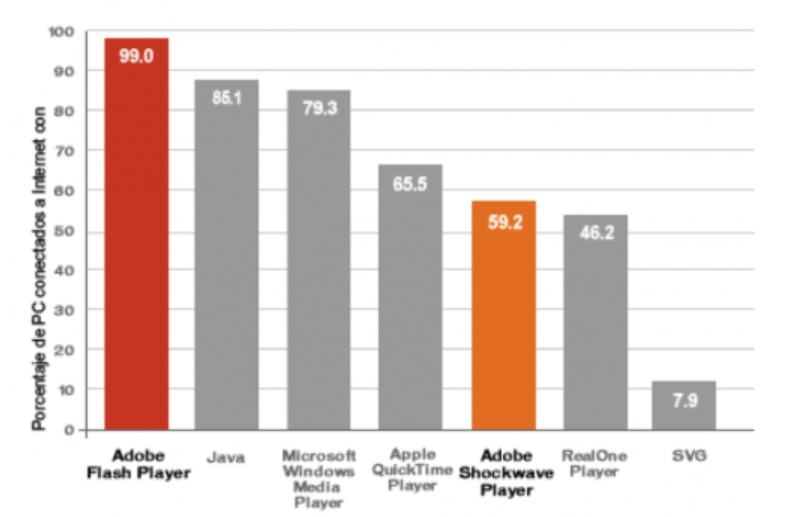
\includegraphics[scale=0.3]{Diseno/RelacionUsuarioAdobeFlashPlayer}}

\caption{Utilización de Adobe Flash Player}
\end{figure}


\textit{Acrobat Connect Professional}\textsuperscript{\textregistered{}}
se basa en una arquitectura abierta y ampliable que permite una integración
rentable con la infraestructura existente y las inversiones futuras
en tecnología\@. \textit{Acrobat Connect Professional}\textsuperscript{\textregistered{}}
utiliza estándares como XML y Java\texttrademark{} para el intercambio
de datos, y es la única solución que admite servicios web que se pueden
usar para la gestión de todos los elementos\@. \textit{Adobe}\textsuperscript{\textregistered{}}
ofrece también un centro de recursos para desarrolladores, con cientos
de interfaces de programación de aplicaciones (API) y kits de desarrollo
de \emph{software} (SDK) para ampliar funciones e integrar la solución
con otras aplicaciones y servicios internos, hasta crear la solución
personalizada que mejor se adapte a las necesidades exclusivas de
la organización\@.

\smallskip{}


La API de \textit{Adobe Connect}\textsuperscript{\textregistered{}}
es sin duda su principal baza para que cualquier desarro\-llador de
aplicaciones web lo elija como motor de videoconferencia\@.

\smallskip{}


\textit{Adobe Connect}\textsuperscript{\textregistered{}} posee
una de las API's más completas para sistemas de videoconferencia,
lo que ofrece la posibilidad de configurar todos los parámetros de
una sala de una forma muy precisa\@. Para este proyecto una de las
funcionalidades más interesante es la posibilidad de configurar las
plantillas de cada sala para adaptar la aplicación a los diferentes
escenarios, ya sean clases magistrales, reuniones de grupos de investigación
con uno o varios ponentes, salas de trabajo en grupo, etc\@. También
ofrece la opción de configurar el ancho de banda que ocupará el flujo
de audio y vídeo de la aplicación en su viaje por la red\@.

\medskip{}



\section{Symfony}

Es uno de los \textit{frameworks }con mayor impacto en la actualidad\@.
Symfony aumenta exponencialmente la productividad y ayuda a mejorar
la calidad de las aplicaciones web aplicando todas las buenas prácticas
y patrones de diseño que se han definido para la web \cite{key-7}\@.
Un gran abanico de aplicaciones web que nacen en la actualidad se
realizan utilizando este \textit{framework,} ya que ofrece una gran
versatilidad y la posibilidad de testear el código con un eficiente
sistema interno para la corrección de errores\@. Symfony también
dota a las aplicaciones de una gran velocidad como se ha comentado
en el apartado \ref{sub:Arquitectura}\@.

\smallskip{}


Su asignador relacional de objetos (ORM) y la capa de abstracción
de base de datos de potente calado y gran capacidad de configuración,
hacen que este \textit{framework} ofrezca al desarrollador la posibilidad
de realizar aplicaciones web basadas en PHP muy sofisticadas\@. Una
de las virtudes más importantes para la elección de este \textit{framework},
es la gran comunidad que lo respalda y que aporta correción de errores
e implantación de tecnologías punteras en sus últimas versiones\@. Por otro lado,
la inmensa y completa documentación web que existe en su web facilita la incorporación al proyecto
de nuevos desarrolladores\@. Las versiones actuales nos garantizan que la evolución de Symfony
guarde una buena estructura de manera que actualizar el antiguo \textit{software}
implementado con Symfony no traerá grandes quebraderos de cabeza\@.

\smallskip{}


El proyecto Doctrine hace que la elección de Symfony sea obvia ante
el desarrollo de cualquier aplicación digna de perdurar en el tiempo\@.
Ofrece un gran abanico de opciones para ampliar la base de datos
y optimizar el tiempo empleado para conseguir las nuevas funcionalidades
en un breve espacio de tiempo y sin un gran despliegue humano\@.
Cualquier tecnología web puede ser incrustada en los ficheros de Symfony
para mejorar o aumentar la compatibilidad entre aplicaciones y necesidades
del usuario final\@. La evolución de Symfony marcada por su creador Fabien Potencier
lleva a este framework a una evolución cada vez más modular en pequeñas funcionalidades,
este hecho facilita la integración de módulos concretos de Symfony en diferentes aplicaciones
sin la necesidad de realizar la aplicación completamente utilizando Symfony. De esta forma
proyectos desarrollados íntegramente en PHP pueden hacer uso de funcionalidades de Symfony
sin realizar una migración completa\@.

\medskip{}



\section{PHP}

Según crecía PHP, empezó a ser reconocido como una popular plataforma
de desarrollo web\@. Una de las más interesantes formas de ver esta
tendencia fue observando los libros de PHP que se han ido publicando
a lo largo de los años\@. Este gran número de libros, escritos por
diferentes autores, publicados por muchos editores, y su disponibilidad
en tantas lenguas son un fuerte testimonio del éxito mundial de PHP
\cite{key-10}\@.

\smallskip{}


Las cuatro grandes características para declinar la balanza hacia
PHP han sido:

\smallskip{}

\begin{itemize}
\item Velocidad: No sólo la velocidad de ejecución, la cual es importante,
sino además no crear demoras en la máquina\@. Por esta razón no debe
requerir demasiados recursos de sistema. PHP se integra muy bien junto
a otro \emph{software}, especialmente bajo ambientes Unix, cuando
se configura como módulo de Apache\@.
\item Estabilidad: La velocidad no sirve de mucho si el sistema no es fiable.
Ninguna aplicación es 100\% libre de errores, pero con una increíble
comunidad de programadores y usuarios como respaldo es mucho mas difícil
que sobrevivan. PHP utiliza su propio sistema de administración de
recursos y dispone de un sofisticado método de manejo de variables,
conformando un sistema robusto y estable.
\item Seguridad: El sistema debe poseer protecciones contra ataques. PHP
provee diferentes niveles de seguridad configurables\@.
\item Simplicidad: Se les debe permitir a los programadores generar código
productivamente en el menor tiempo posible. Usuarios con experiencia
en C y C++ podrán utilizar PHP rápidamente\@. No cabe la menor duda
de que la utilización de un \textit{framework} simplifica todavía
más su utilización\@.
\end{itemize}
\smallskip{}


Este conjunto de dogmas unidos a la gran comunidad que desarrolla
PHP y ayuda a incluir las funcionalidades de última generación, hacen
de PHP el \emph{software} recomendado para el servidor Apache, que
como describiremos a continuación hacen un fantástico equipo, altamente
recomendado para la puesta en servicio de aplicaciones web\@.

\medskip{}



\section{Apache}

La elección del servidor web Apache se debe a las siguientes ventajas:

\smallskip{}

\begin{itemize}
\item Modular:


Podemos incluir multitud de módulos para adecuar el servidor a las
necesidades de la aplicación\@. De hecho, PHP posee un módulo
específico para Apache, como ya se ha comentado en el capítulo \ref{chap:Tecnolog=0000EDas-empleadas},
que aprovecha al máximo la velocidad ya que actúa sobre
el núcleo del servidor de forma directa\@.

\item Código abierto:


Las plataformas de código abierto nos permiten desarrollar código
de forma libre y a un menor coste que el \emph{software} propietario\@.
Los foros de discusión y resolución de errores son mucho mayores,
de forma que un desarrollador puede encontrar solución a su problema
de forma rápida y en caso de ser pionero en una casuística determinada,
también obtendrá respuesta de forma rápida, ya que la comunidad libre
es muy activa\@.

\item Multi-plataforma:


Es imprescindible para cualquier aplicación poder desplegarse en todo
sistema operativo existente en el mercado, y esta premisa la cumple
Apache a la perfección\@.

\item Extensible:


Consta de una amplia galería de módulos que hacen que podamos agregar
multitud de funcionaliades, como el ya mencionado y utilizado en este
proyecto módulo para PHP\@.

\item Popular:


Gracias a su popularidad que crece día a día debido a su licencia,
cualquier desarro\-llador cuenta con una amplia comunidad que lo respalda
y aumenta la actividad tanto de desarrolladores como de expertos en
este servidor\@.

\end{itemize}
\medskip{}



\section{MySQL}

Son muchas las razones para escoger MySQL como solución de misión
crítica para la administración de datos\@. Las más interesantes ligadas
a este proyecto son:

\smallskip{}

\begin{itemize}
\item Coste: El coste de MySQL es gratuito en su mayor parte y su servicio
de asistencia resulta económico en caso de ser necesario\@.
\item Asistencia: MySQL AB, la compañía responsable del desarrollo de MySQL,
ofrece contratos de asistencia a precios razonables y existe una nutrida
y activa comunidad MySQL\@.
\item Velocidad: MySQL es mucho mas rápido que la mayor parte de sus rivales,
por tanto en este aspecto es obvia su elección\@.
\item Funcionalidad: MySQL dispone de muchas de las funciones que exigen
los desarro\-lladores profesionales, como compatibilidad completa con
ACID, compatibilidad para la mayor parte de SQL ANSI, volcados online,
duplicación, funciones SSL e interacción con la mayor parte de los
entornos de programación. Se desarrolla y actualiza mas rápidamente
que la mayoría de sus rivales, por lo que prácticamente todas las
funciones estándar de MySQL no están en fase de desarrollo\@.
\item Portabilidad: MySQL se ejecuta en la inmensa mayoría de sistemas operativos
y, en la mayor parte de los casos, los datos se pueden transferir
de un sistema a otro sin dificultad\@.
\item Facilidad de uso: MySQL resulta fácil de utilizar y de administrar.
Gran parte de las viejas bases de datos presentan problemas por utilizar
sistemas obsoletos, lo que complica innecesariamente las tareas de
administración\@. Las herramientas de MySQL son potentes y flexibles,
sin sacrificar su capacidad\@.
\end{itemize}
\smallskip{}


MySQL 5.5 es rápido, dispone de funciones de volcado online e incorpora
una gran cantidad de funciones nuevas\@. Son pocas las razones para
desechar MySQL como solución de base de datos\@.

\smallskip{}


MySQL AB dispone de un sistema de asistencia eficiente y a un precio
razonable, y, como ocurre con la mayor parte de las comunidades de
código abierto, hay disponible una gran cantidad de ayuda en la web\@.

\smallskip{}


Junto con el visor de base de datos TOra que permite la edición de
la base de datos de una forma sencilla, facilitando la búsqueda visual
de datos para su depuración y mayor facilidad en el diseño, hacen
de estas dos herramientas la mejor opción disponible en el mercado
relación calidad-precio para el desarrollo de aplicaciones web y cada
vez más en otros sectores\@.


\chapter{Implementación del proyecto\label{chap:Desarrollo-del-proyecto}}

La aplicación eMeeting está diseñada para crear salas de forma
dinámica bajo demanda y acceder a las mismas de forma similar a una
llamada telefónica, es decir, en el momento de acceso se consulta
la disponibilidad de recursos y se deniega el acceso en el peor de
los casos\@. En la creación de la sala se pueden seleccionar los
usuarios que participarán en la videoconferencia de una lista obtenida
de la base de datos o definir metadatos característicos de una sala como 
el nombre o una breve descripción para convertir la sala en única\@. El
número máximo de conferencias simultáneas es una limitación para la aplicación,
ya que el \emph{software} propietario aumenta su coste con el incremento de salas\@.
Sin embargo, en el diseño se ha supuesto que nunca se llegará a tal número y se han dimensionado
las conexiones con un criterio que garantice un bajo porcentaje de
bloqueo de petición de conexión, para lo cual se realizará un interfaz
de seguimiento que mostrará estadísticas con el número máximo de videoconferencias
simultáneas, número de usuarios en activo y otros parámetros de interés\@.
De esta forma la lógica del número máximo de salas será transparente
para el usuario\@.

\smallskip{}


En este capítulo se describirán las entidades, repositorios, controladores
y servicios de la aplicación\@. Cada una de estas partes es fundamental
y el propio \textit{framework} nos ofrece cómodas herramientas para
obtener un modelo vista controlador (MVC) funcional y de fácil implementación\@.
Las entidades definen las tablas de la base de datos\@. En los repositorios
se almacenan las consultas a la base de datos que no genera el \textit{framework}
por defecto\@. Los controladores contienen la lógica que procesará
los datos de la aplicación y tienen asociadas las plantillas para
mostrar o recoger los datos introducidos por el usuario\@. Los servicios
contienen las funciones que usan la API \textit{Adobe Connect}\textsuperscript{\textregistered{}}
y proporcionan a eMeeting las credenciales necesarias para conectarse
como administrador al servidor \textit{Adobe Connect}\textsuperscript{\textregistered{}}
y generar las salas, usuarios y todo lo necesario para el correcto
funcionamiento de la aplicación\@.

\smallskip{}


Para llevar a cabo la aplicación se ha dispuesto de cinco elementos\@.
Como se puede observar en la figura \ref{Estruc_aplicacion}, contamos
con un cliente que representa el conjunto de usuarios involucrados
en la comunicación que disfrutan de la aplicación desde su explorador
web, aunque también es posible operar desde un terminal móvil previa
descarga de un \textit{plugin}, y cuatro servidores que se detallan
a continuación\@.

\begin{figure}
\centerline{\includegraphics[scale=0.6]{Diseno/Esquema_aplicacion}}

\caption{Diagrama estructural de la aplicación}
\label{Estruc_aplicacion}
\end{figure}

\newpage

\begin{itemize}
\item El servidor eMeeting: almacena todos los ficheros necesarios para
la configuración y el funcionamiento de la aplicación web\@.
\item La base de datos de respaldo de la aplicación: que en este caso se
implementa utilizando el motor MySQL\@. El diseño de la aplicación
permite modificar el motor de base de datos realizando cambios
exiguos\@.
\item Directorio +: este servidor ayudará a sincronizar la macroaplicación
mencionada en la sección \ref{sec:Objetivos} y que se describirá
con mayor detalle en este capítulo\@. La base de datos de respaldo
sería redundante pero en la fase de despliegue y puesta en servicio
es aconsejable para aportar una mayor fiabilidad y estabilidad al
servicio\@. En caso de mantenerla, la velocidad de la aplicación aumentará
al liberar al servidor Directorio + de las consultas que se realicen sobre
la base de datos alojada en el servidor eMeeting\@.
\item El servidor \textit{Adobe Connect}\textsuperscript{\textregistered{}}:
donde se encuentra alojada la aplicación \textit{Adobe Co\-nnect}\textsuperscript{\textregistered{}}
que se usará como motor de videoconferencia\@.
\item El servidor CAS: aloja el servicio para autenticar a los usuarios
que accedan a la aplicación y ayudará a ``Directorio +'' a detectar
usuarios ya registrados en alguna aplicación para evitar registros
superfluos en el resto de aplicaciones que componen ``Campus do Mar''\@.
\end{itemize}
\medskip{}



\section{Archivos de configuración}

Los archivos de configuración están almacenados en diferentes carpetas
dentro de los directorios Symfony descritos en la subsección \ref{sec:SYMFONY}\@.

\smallskip{}


En el interior del directorio app/config se encuentran dos ficheros
importantes: \textit{rou\-ting.yml} y \textit{security.yml}\@. Este
par de ficheros, contienen la configuración que determina qué URLs
de acceso a la aplicación serán públicas o privadas y cuál será la
puerta de entrada para las URLs privadas que se describirán en la
subsección \ref{sec:URLs-de-acceso}\@.

\smallskip{}


En la carpeta \textit{Resources/public/css} guardaremos los archivos
para alojar el CSS, en \textit{Resources/public/js} el Javascript,
en \textit{Resources/public/images} las imágenes y en \textit{Resources/pu\-blic/wsdl}
la configuración de las funciones del \textit{middleware} que describiremos
en la subsección \ref{sub:El-Middleware}\@.

\smallskip{}


En la carpeta \textit{Resources/views} se almacenan las plantillas
que se mostrarán en el explorador para cada uno de los controladores
de aplicación debidamente ordenados según corresponda\@. En el interior
de este directorio se aloja una carpeta por cada controlador, con
archivos que procesan la información ofrecida por los controladores para
mostrar o recoger datos en cada plantilla HTML\@.

\smallskip{}


En la carpeta \textit{Test} se almacenan archivos para diseñar pruebas
específicas para cada controlador, entidad y servicio de la aplicación
agrupadas en directorios con nombres re\-lativos a los elementos sobre
los cuales se ejecutarán las pruebas\@. En el interior de cada uno
de estos tres directorios están disponibles los ficheros para realizar
pruebas diseñadas por el programador que intentan detectar errores,
fallos de diseño o puntos débiles de la aplicación\@. Esta funcionalidad
de Symfony ha revelado una gran cantidad de errores en el código,
\textit{a priori} muy difíciles de detectar\@.

\medskip{}



\section{Concepto de sala\label{sec:Concepto-de-sala}}

Se llama sala a la entidad fundamental de la aplicación\@. Cada sala
contendrá una única reunión en la que todos los participantes colaboran
según el rol que desempeñen\@. Cada usuario podrá crear las salas
que precise oportunas y darle el nombre que desee, aunque el número
total de salas en uso no podrá superar diez, en el caso de ``Campus do Mar'',
aunque puede modificarse en los ficheros de configuración, pero esta información
será transparente al usuario y una lógica interna ha sido diseñada
para alertar al administrador de la aplicación sobre la proximidad
al número máximo de salas en uso, por si cree oportuno disponer de
más salas y debe negociarlo con la compañía suministradora de recursos,
en el caso de este proyecto \textit{Adobe Connect}\textsuperscript{\textregistered{}}\@.
La aplicación eMeeting podría utilizarse con otro motor de videoconferencia,
pero sería de todas formas necesario informar al administrador de
la proximidad del número máximo de salas en uso, ya que en cualquier
motor el número de salas es un recurso limitado\@. Un inconveniente
de la aplicación es no poder dar un nombre de sala que exista de entre
las salas en activo. Sería posible implementar una lógica para que
cada usuario no se percate en primera instancia de este hecho, ya
que \textit{Adobe Connect}\textsuperscript{\textregistered{}}\textsuperscript{}
no permite tener salas con el mismo nombre, pero esta solución cambiará
el nombre de la sala en la pantalla de \textit{Adobe Connect}\textsuperscript{\textregistered{}}\textsuperscript{},
por este motivo no se ha implementado esta funcionalidad\@.

\begin{figure}
\centerline{\includegraphics[scale=0.45]{\string"Fotos de eMeeting/HelpMeeting\string".png}}

\caption{Ayuda de la aplicación}


\label{HelpMeeting}
\end{figure}


El concepto de sala no se refleja en la lógica de la base de datos,
aunque podría asociarse a la tabla \textit{meeting} ya que cada las reuniomes se realizan en una sala,
pero se tiene muy presente a la hora de diseñar y mostrar la aplicación
al usuario\@. Podría decirse que una reunión se realiza en una sala,
pero en realidad disponemos únicamente de diez salas, sin embargo
el usuario puede crear todas las reuniones que desee\@. En los primeros
diseños, de forma transparente al usuario, se creaba una sala de videoconferencia
para cada usuario de ``Campus do Mar'', y se mostraba al usuario
los estados de sala (\textit{room}) habilitada/deshabi\-litada, mágica/no
mágica o secreta/pública. Definitivamente este diseño se abandonó
y el usuario entra por primera vez a la aplicación y no posee ninguna
sala, una enorme flecha le inidica las instrucciones a seguir para
crear su propia sala como se puede ver en la figura \ref{FirsTimeAccess}\@.
También se dispone de un manual en red con indicaciones para realizar
cualquier acción disponible dentro de la aplicación eMeeting,
ver figura \ref{HelpMeeting}\@. En la lógica de base de datos,
las salas libres son en realidad reuniones (\textit{meetings}) almacenadas
en la tabla \textit{meeting} y siempre
están asociadas a un estado: \textit{NOW, NEW, SCHEDULE, CANCELLED, FINICHED o LOCKED}\@.
Estos seis estados, que se explicarán con detalle en la sección \ref{sec:Dise=0000F1o-de-la},
son fundamentales para gestionar las funcionalidades que ofrece la
aplicación\@.

\begin{figure}
\centerline{\includegraphics[scale=0.5]{\string"Fotos de eMeeting/Fotos antiguas/inciosineMeetings\string".png}}

\caption{Pantalla de inicio por vez primera a la aplicación.}


\label{FirsTimeAccess}
\end{figure}



\subsection{Sala mágica\label{sub:Sala-m=0000E1gica}}

Una sala mágica hace referencia a un tipo especial de sala que se
pone a disposición de los usuarios de la aplicación para proporcionar
un servicio exclusivo\@. Como se ha comentado en este capítulo el
número de salas disponibles es limitado y cabe la posibilidad de denegación
de servicio en momentos de máxima ocupación\@. Como se describirá
con mayor profundidad en la subsección \ref{sub:Recopilaci=0000F3n-de-datos}
el sistema alerta al administrador para que provisione con más salas
a la aplicación si la ocupación se acerca al límite máximo disponible\@.
Debido a esta implementación y ante saturación no deseada se ha implementado
una lógica que recibe el nombre de sala mágica\@.

\smallskip{}


A partir de la lista total de licencias disponibles se configura el
número máximo de salas mágicas\@. El sistema podría permitir configurar
todas las licencias como mágicas aunque es una opción absurda ya que
la finalidad del diseño de este sistema consiste en proporcionar muchas
entidades eMeeting a cada usuario con una disposición
de licencias limitada, este hecho lleva al administrador a fijar un
número máximo de salas mágicas en los ficheros de configuración\@.
Cualquier sala del sistema puede ser marcada como mágica por el administrador
y por tanto pasará a estar siempre disponible, por contra una licencia
estará siempre ocupada y no disponible para el resto de usuarios\@.
Para entender mejor esta lógica pasamos a describir el caso concreto
de ``Campus do Mar''\@.

\smallskip{}


Existen diez licencias y tres salas mágicas como máximo\@. Cuando
se marca una sala como mágica las licencias disponibles para el resto
de usuarios pasan a ser nueve ya que la sala marcada como mágica ocupa
la licencia en todo momento incluso cuando no hay una reunión en curso\@.
De esta forma se garantiza la disponibilidad del recurso en detrimento
del número de salas disponibles\@. Este tipo de salas permite al
administrador del sistema asegurarse la disponibilidad de recursos
incluso en periodos de máxima ocupación y ofrecer un servicio exclusivo
a usuarios con un perfil determinado\@.

\medskip{}



\subsection{Acceso a las salas\label{sub:Acceso-a-las}}

Debido a los diferentes tipos de salas y roles de usuario es necesario
implementar un control de acceso a las salas\@. Para esta lógica
se definen los conceptos de \textit{Viewsalt}, \textit{Salt} y \textit{SecretSalt},
que facilitarán la construcción de las URLs de acceso a las diferentes
salas de la aplicación\@.

\smallskip{}

\begin{itemize}
\item \textit{Viewsalt}: Se genera con el algoritmo MD5, a partir del nombre
que recibe la reunión\@. Se describe con mayor detalle en la sección
\ref{sec:URLs-de-acceso}\@. La URL con esta huella dará acceso a
las reuniones públicas mediante registro a través del formulario correspondiente
para actuar en la reunión como un usuario participante (\emph{participant})
descrito en la subsección \ref{sub:Definici=0000F3n-de-roles}\@.
\item \textit{Salt}: Este campo que se almacena asociado a cada una de
las reuniones creadas, es generado a partir del nombre de usuario\@. Construye la URL de acceso
para las salas públicas y usuarios presentadores (\emph{presenter})
descritos en la subsección \ref{sub:Definici=0000F3n-de-roles}\@.
\item \textit{SecretSalt}: Se genera con el algoritmo MD5 a partir del
nombre de usuario o del nombre de grupo\@. Construye las URLs para
las salas privadas\@. Este acceso es realmente importante ya que
una sala privada no posee un enlace común de acceso y sólo los usuarios
invitados pueden acceder a ella\@. Este enlace permite el acceso
a la sala a todo usuario que lo posea a pesar de ser una sala privada,
por así decirlo es como una puerta trasera a una sala que por definición
no es accesible a usuarios no invitados\@.
\end{itemize}
\smallskip{}


El acceso a cada sala se decide en el momento de creación de la misma\@.
Para el servidor \textit{Adobe Connect}\textsuperscript{\textregistered{}}\textsuperscript{} todas
las salas serán públicas lo que permite gestionar el control de acceso
desde la propia aplicación eMeeting\@. De esta forma a
partir de la URL generada el usuario puede decidir invitar a cualquier
persona, ya sea miembro de la Plataforma ``Campus do Mar'' o no
y otorgarle el rol que considere oportuno\@. Este planteamiento es
altamente útil para dar una mayor flexibilidad a la hora de trabajar
con personal ajeno a ``Campus do Mar'', pero que en un momento dado
puede colaborar en un proyecto determinado\@.

\smallskip{}


Este control de acceso se implementa con la siguiente lógica según el tipo de sala:

\smallskip{}

\begin{itemize}
\item Pública: 

\begin{itemize}
\item Entrada con \textit{Salt}: Pueden entrar los usuarios que conozcan la sala
del usuario ya que la URL se construye a partir del nombre de la sala\@.
\item Entrada con \textit{SecretSalt}: Pueden entrar todos los que conozcan la URL
generada a partir del \textit{SecretSalt} de la sala\@.
\end{itemize}

\newpage

\item Privada: 

\begin{itemize}
\item Entrada con \textit{Salt}: Sólo puede entrar el usuario\@. Esta situación
se genera como consecuencia de la lógica implementada, pero es absurdo
el hecho de una reunión para un sólo usuario\@.
\item Entrada con \textit{SecretSalt}: Pueden entrar todos los que conozcan la URL
generada con el \textit{SecretSalt} de la sala\@.
\end{itemize}
\end{itemize}
\medskip{}



\section{CRON\label{sec:CRON}}

El cron es la parte del servidor eMeeting que se encarga de
ejecutar funciones periódicas que ayudan a la sincronización, depuración
y mantenimiento de la aplicación\@. Cada una de estas funciones realiza
tareas críticas para el correcto funcionamiento de la aplicación y
alerta a los administradores de posibles saturaciones en el servicio\@.

\smallskip{}


A continuación se describen las funciones ejecutadas por el
cron\@.

\medskip{}



\subsection{Sincronización de grabaciones}

Para poder visualizar las grabaciones en tiempo real y antes de eliminar
la reunión, se ejecuta el comando \textsc{cmar:sync:rec} diseñado
para guardar en la base de datos la URL de acceso a las grabaciones
únicamente cuando la grabación ha finalizado\@.

\smallskip{}


Esta acción es ejecutada cada cinco minutos por el cron, comprueba
las grabaciones finalizadas y almacena las URLs de acceso a las mismas
en la base de datos quedando disponibles en el botón \emph{All Recordings}
que se describirá en la subsección \ref{sub:Botonera-para-cada}\@.

\smallskip{}


La acción de borrado de la reunión finaliza ejecutando esta acción
para almacenar todas las grabaciones en una carpeta creada para tal
efecto dentro del servidor de \textit{Adobe Connect}\textsuperscript{\textregistered{}}\textsuperscript{}\@.
Las grabaciones nunca se eliminan del servidor y siempre son accesibles
por el usuario desde la botonera superior que describiremos en la
subsección \ref{sub:Botonera-superior-de}\@.

\medskip{}



\subsection{Sincronización de usuarios de \textit{Adobe Connect}\textsuperscript{\textregistered{}}\textsuperscript{}}

Cuando un usuario accede a una sala y no tiene una cuenta de acceso
a la aplicación, se crea un usuario temporal en \textit{Adobe Connect}\textsuperscript{\textregistered{}}\textsuperscript{}\@.
Esta medida nos otorga control total sobre los privilegios de los
participantes en la reunión\@. Este diseño es necesario puesto que
\textit{Adobe Connect}\textsuperscript{\textregistered{}}\textsuperscript{}
no ofrece ninguna solución en su API para abordar esta casuística,
aunque se ha comprobado que internamente sí están implementados diferentes
roles para usuarios anónimos\@. Dicho comando se llama \textsc{cmar:sync:userADO}\@.

\smallskip{}


El usuario, creado para dar solución a este problema, es borrado dos
días después de su creación\@. Para ello en el campo descripción
que ofrece \textit{Adobe Connect}\textsuperscript{\textregistered{}}\textsuperscript{}
se incluye el texto: \textit{User created as guest} y en el campo
reservado para la dirección de correo electrónico se incluye la fecha
de creación para eliminar este tipo de usuarios a su debido tiempo\@.

\medskip{}



\subsection{Recopilación de datos para la elaboración de estadísticas de la aplicación\label{sub:Recopilaci=0000F3n-de-datos}}

Este script se ejecuta cada treinta minutos y recoge información sobre
el número de salas activas y el número de usuarios en cada sala para
elaborar estadísticas de uso del sistema\@. La función más importante
consiste en comparar el número de salas activas con el número máximo
contratado y alertar al administrador de la proximidad entre ambos
ya que \textit{Adobe Connect}\textsuperscript{\textregistered{}}\textsuperscript{}
ofrece licencias de pago que se han de contratar previamente\@. Si
se da el caso, el administrador debe ampliar el número de licencias
para evitar que usuarios no puedan disfrutar de su multivideoconferencia\@.
Este comando recibe el nombre de \textsc{cmar:sync:storestat}\@.

\medskip{}



\section{Diseño de la base de datos\label{sec:Dise=0000F1o-de-la}}

Uno de los primeros desafíos que se han superado es el diseño de
la base de datos\@. Como se indicó en el capítulo \ref{chap:Dise=0000F1o-del-proyecto}
con el \textit{framework} Symfony es fácilmente implementable e incluso
puede modificarse durante la fase de prueba, en caso de encontrar
alguna carencia en el diseño inicial\@. La utilización de MySQL,
gracias a su velocidad, nos augura un desarrollo exitoso\@. A pesar
de ello, con la aplicación en producción, modificar la base de datos
puede ocasionar enormes quebraderos de cabeza\@. Como consecuencia
de este hecho, implementar una base de datos sólida con la información
más relevante para la aplicación es una labor tediosa que se
ha elaborado con gran detenimiento\@.

Symfony ofrece al desarrollador las entidades y repositorios para
simplificar la labor de diseño de la base de datos como se explicó
en el capítulo \ref{chap:Tecnolog=0000EDas-empleadas}\@. En las
entidades se definirán los campos que se guardarán en la base de datos
y Symfony por defecto creará una serie de sentencias sencillas para
obtener valores de las tablas de la base de datos, tales como el nombre
de una reunión, su identificador o el usuario creador\@. Como en
toda aplicación web hay una serie de consultas complejas necesarias
para la aplicación que no implementa el \textit{framework}, por
ello en los repositorios de las entidades se implementan este tipo
de consultas\@. La entidad es un tipo de dato propio de Symfony que
permite acceder a las columnas de una tabla\@. De esta forma cuando
una consulta a la base de datos devuelve una entidad se tendrá acceso
a todos los valores de la fila correspondiente utilizando las consultas
que Symfony crea por defecto para la entidad\@.

\smallskip{}


A continuación se describen las entidades y sus respectivos repositorios\@.

\smallskip{}


\begin{figure}[h]
\centerline{\includegraphics[scale=0.5]{\string"Diseno/Imagenes base de datos/Meeting\string".png}}

\caption{Tabla para almacenar datos de reuniones}
\label{Tabla_eMeeting}
\end{figure}

\begin{itemize}
\item Meeting


A continuación y a modo de ejemplo se muestra el archivo de la entidad
\textit{meeting}, sin duda la más importante de la aplicación, y que nos dará
una idea de la estructura de la base de datos\@. A partir de la tabla
que genera este código se dispondrá de una visión más clara de las
funciones que se describirán para el interfaz de usuario\@. Las variables
de esta tabla almacenan los diferentes estados en los que puede encontrarse
una reunión, los identificadores de reunión o datos de creación\@.


\medskip{}

\begin{lstlisting}

/**
* @var integer $id
*
* @ORM\Column(name=``id'', type=``integer'')
* @ORM\Id 
* @ORM\GeneratedValue(strategy=``AUTO'')
*/
private $id;


/** 
* @var integer $state 
*
* @ORM\Column(name=``state'', type=``integer'')
*/
private $state = self::STATE_NEW;


/**
* @var string $salt 
* 
* @Assert\NotBlank() 
* @ORM\Column(name=``salt'', type=``string'', length=255, nullable=false) 
*/
private $salt; 


/** 
* Link para entrar como usuario mini-host en ADO 
* @var string $secretsalt
* 
* @Assert\NotBlank() 
* @ORM\Column(name=``secretsalt'', type=``string'', length=255, nullable=false)
*/
private $secretsalt; 


/** 
* Link para entrar como usuario view en ADO
* @var string $viewsalt 
*
* @Assert\NotBlank()
* @ORM\Column(name=``viewsalt'', type=``string'', length=255, nullable=false)
*/
private $viewsalt;


/** 
* @var string $title 
* 
* @Assert\NotBlank() 
* @ORM\Column(name=``title'', type=``string'', length=255, nullable=false)
*/
private $title;


/** 
* @var text $description 
* 
* @ORM\Column(name=``description'', type=``text'', nullable=true) 
*/
private $description;


/** 
* @var string $URL
* 
* @ORM\Column(name=``URL'', type=``string'', length=255, nullable=true) 
*/
private $URL; 


/** 
* @var string $title 
* 
* @Assert\NotBlank() 
* @ORM\Column(name=``title'', type=``string'', length=255, nullable=false)
*/ 
private $title; 


/** 
* @var text $description 
* 
* @ORM\Column(name=``description'', type=``text'', nullable=true)
*/
private $description;


/** 
* @var string $URL 
* 
* @ORM\Column(name=``URL'', type=``string'', length=255, nullable=true) 
*/
private $URL; 


/** 
* @var datetime $date
* 
* @ORM\Column(name=``date'', type=``datetime'')
*/
private $date;


/**
* @var boolean $public
* 
* @ORM\Column(name=``public'', type=``boolean'', nullable=true)
*/
private $public;


/**
* @var boolean $public
* 
* @ORM\Column(name=``magic'', type=``boolean'', nullable=false)
*/
private $magic; 


/** 
* @var User $owner
*
* @ORM\ManyToOne(targetEntity=``User'', inversedBy=``id'')
* @ORM\JoinColumn(name=``owner_id'', referencedColumnName=``id'')
*/ 
private $owner; 


/** 
* @var Group $group 
*
* @ORM\ManyToOne(targetEntity=``Group'', inversedBy=``id'', cascade={``remove''})
* @ORM\JoinColumn(name=``group_id'', referencedColumnName=``id'') 
*/ 
private $group = null;


/**
* @var ArrayCollection $users
*
* @ORM\ManyToMany(targetEntity=``User'', cascade={``remove''})
* @ORM\JoinTable(name=``meeting_user'',
*      joinColumns={@ORM\JoinColumn(name=``meeting_id'', referencedColumnName=``id'')},
*      inverseJoinColumns={@ORM\JoinColumn(name=``user_id'', referencedColumnName=``id'')}
*      ) 
*/ 
private $users;


/** 
* @var ArrayCollection $recordings 
*
* @ORM\OneToMany(targetEntity=``Recording'', mappedBy=``meeting'', cascade={``remove''}) 
*/ 
private $recordings; 


/** 
* @var ArrayCollection $recordings 
* 
* @ORM\OneToMany(targetEntity=``NickName'', mappedBy=``meeting'', cascade={``remove''})
*/
private $nicknames;


/** 
* @var integer $concurrent 
* 
* @ORM\Column(name=``concurrent'', type=``integer'')
*/ 
private $concurrent = 0;


/** 
* @var datetime $created 
*
* @ORM\Column(name=``created'', type=``datetime'') 
*/ 
private $created;


/**
* @var datetime $updated 
*
* @ORM\Column(name=``updated'', type=``datetime'') 
*/ 
private $updated; 


\end{lstlisting}

\begin{itemize}
\item Función que introduce datos al crear una reunión nueva:


\begin{lstlisting}
public function __construct(User $owner = null) { 
 $this->owner = $owner;
 $this->created = $this->updated = new  DateTime(``now''); 
 $this->date = new DateTime(``tomorrow''); 
 $this->users = new \Doctrine\Common\Collections\ArrayCollection(); 
 $this->recordings = new \Doctrine\Common\Collections\ArrayCollection(); 
}
\end{lstlisting}

\item Función que devuelve el título de la reunión en forma de cadena de
texto cuando se solicita el título de dicha varible con la sentecia
\texttt{\$variable->getTitle()}:


\begin{lstlisting}
public function __toString() {
   return $this->title;
}
\end{lstlisting}

\item Función que devuelve el estado de la reunión.


Para cada una de las variables definidas en la entidad, se tiene una
función get y set para recuperar o guardar la variable en el momento
que se precise y que será transparente para diferentes bases de datos,
ya que el \textit{framework} se encargará de construir la petición
según la base de datos que se introduzca en el fichero de configuración\@.

\end{itemize}

Para las consultas que se almacenan en los repositorios se aconseja
que devuelvan una entidad del tipo al cual pertenezcan, es decir, las
consultas del repositorio de la entidad reunión (\emph{meeting}) devuelven
entidades \emph{meeting}, aunque no es obligatorio el orden es importante
para depurar código\@. El repositorio de esta entidad posee las funciones
que se describen a continuación:
\begin{itemize}
\item \texttt{findByStateAndUser}: devuelve una entidad \emph{meeting} a
partir de un estado de reunión y una entidad usuario (\emph{user})\@.
La reunión debe encontrarse en el estado enviado a la consulta y pertenecer
al usuario que se corresponde con dicha entidad\@.
\item \texttt{findByUserAndStatesOrderByRank}: a partir de una entidad \emph{user}
y una lista de estados devuelve entidades \emph{meeting} según el
orden de la columna ``rank''\@.
\item \texttt{findByStates}: selecciona entidades \emph{meeting} que se
encuentren en alguno de los estados que se envían a la función\@.
\item \texttt{findByStatesAndMagicRoom}: recibe como parámetros una lista
de estados y un \emph{booleano}, según se precise que las entidades
\emph{meeting} de retorno sean mágicas o no\@. Es obvio que las entidades
se encontrarán en alguno de los estados de la lista\@.
\item \texttt{findOneByStateAndTitle}: devuelve una única entidad a partir
de un estado y un título de reunión\@. Las funciones que comienzan
por \emph{findOne} poseen una ca\-racterística especial proporcionada
por \emph{Symfony}, esta característica consiste en proporcionar un
error específico en caso de que se encuentre en la base de datos más
de un usuario, es por ello, que se utiliza para realizar peticiones
en las cuales se necesita un error en caso de existir más de una respuesta\@.
\item \texttt{findOneByStatesAndTitle}: devuelve una única entidad a partir
de un lista de estados y un título de reunión\@.
\item \texttt{findByStateAndUser}: devuelve entidades \emph{meeting} a partir
de un estado y una entidad \emph{user\@.}
\item \texttt{findByStatesAndUser}: devuelve entidades \emph{meeting} a
partir de una lista de estados y una entidad \emph{user}\@.
\item \texttt{findByStateAndGroup}: esta consulta devuelve entidades \emph{meeting}
con un estado determinado y pertenecientes a un grupo concreto\@.
\item \texttt{findByStateUserAndNotGroup}: esta consulta ofrece entidades
\emph{meeting} con un estado determinado que pertenecen a un usuario
concreto y que no pertenecen al grupo que se pasa como parámetro\@.
\item \texttt{findByStatesAndUserGroup}: devuelve entidades que pertenecen
a la lista de estados, al usuario y grupo que se pasan como parámetros\@.
\item \texttt{findByStatesUserAndMonth}: devuelve entidades que se encuentran
en algún estado de la lista que se pasa como parámetro\@. También
deben pertenecer al usuario enviado y ser creadas en el mes
que se le envía a la función\@. Para ello se suma un mes al mes enviado
y la petición solicita que la columna ``date'' sea mayor que el mes
enviado y menor que la variable a la cual se ha sumado dicho mes\@.
\item \texttt{findByStatesUserAndMonthGroup}: devuelve entidades \emph{meeting}
que se encuentren en algún estado de la lista enviada, que pertenezcan
al usuario que se pasa a la función, que se haya creado en el mes
y pertenezca al grupo que se pasan como parámetros\@.
\item \texttt{findMonthsAndRecordings}: esta es una consulta algo más compleja
que devuelve una lista de datos en formato tabla en la cual por cada
fila tendremos tres columnas para poder mostrar el desplegable del
botón \emph{All Recordings} que se muestra en la figura \ref{RecordsUser}\@.
Esta consulta devuelve para un mes del año y un usuario determinado
el número de reuniones y de grabaciones pertenecientes a dicha reunión
para poder mostrarlo en el menú de la figura mencionada\@. De esta
forma y desplegando este menú se tendrá un acceso rápido al número
de reuniones y grabaciones por mes para acceder más rápidamente a
ellas a partir de la ventana emergente que se muestra al pulsar el
botón \emph{All Recordings\@.}
\item \texttt{findMonthsAndRecordingsGroup}: función idéntica a la anterior
con la salvedad de que la entidad solicitada debe pertenecer a un grupo determinado\@.
\item \texttt{findByStateAndNotUser}: devuelve entidades \emph{meeting}
en un estado determinado, para las cuales el propietario no es el
usuario que se pasa como parámetro\@.
\item \texttt{findHistoricalByUser}: devuelve una lista de entidades cuya
fecha de creación es inferior a la actual y pertenecen al usuario
que se pase como parámetro a esta función\@.
\item \texttt{findOneBySaltOrSecretSalt}: devuelve la entidad \emph{meeting}
única que contenga en su parámetro \emph{salt} o \emph{secretsalt}
el pasado como variable, para hacer la consulta sobre cada uno de
los parámetro se envía a la función un \emph{booleano} que determinará
si se solicita el \emph{salt} o el \emph{secretsalt}\@.
\item \texttt{findOneByViewSalt}: devuelve la entidad \emph{meeting} unívocamente
identificada por su parámetro \emph{viewsalt}\@.
\end{itemize}

En la figura \ref{Tabla_eMeeting} se observan los diferentes campos
que incluye la entidad \textit{meeting}\@.


A continuación, se describe el cometido de las diferentes columnas
de la tabla\@.


\smallskip{}

\begin{itemize}
\item El campo ``id'' se genera de forma automática al introducir un elemento
en la tabla e identifica cada entidad \textit{meeting} dentro de la base
de datos de forma única, requisito impuesto por el motor MySQL para
identificar los contenidos de cada tabla\@.
\item En la columna ``owner\_id'' se almacena el identificador correspondiente
al pro\-pie\-tario y creador de cada reunión\@.
\item ``Group\_id'' se corresponde con una funcionalidad \textit{Out of Scope}\footnote{Fuera de los objetivos de la versión final.},
por lo tanto no se ha utilizado en la actual versión del proyecto,
pero está reservada para una funcionalidad en la que una reunión puede
pertenecer a un grupo de usuarios además de al usuario creador\@.
\item La columna ``state'' almacena el estado de cada reunión que puede
ser \textit{NOW, NEW, SCHEDULED, CANCELLED, FINISHED o LOCKED}\@. 

\begin{itemize}
\item El estado \textit{NOW} indica que la reunión está siendo creada y
ayuda a sincronizar la base de datos ante tiempos de demora. También
se llega a este estado cuando una reunión con duración y fecha está
en curso en el momento actual\@.
\item El estado \textit{NEW} se corresponde con aquel en el cual una reunión
está disponible pero no se le ha dado una fecha ni una duración\@.
La mayoría de las reuniones se encuentran en el estado \textit{NEW}\@. 
\item El estado \textit{SCHEDULED} informa de que la reunión tendrá lugar
en el futuro\@. 
\item La reunión \textit{CANCELLED} es aquella que ha sido creada y luego
borrada\@. La aplicación almacena datos para posteriores estadísticas\@. 
\item El estado \textit{FINISHED} indica que la reunión ha finalizado,
funcionalidad desarrollada para la versión en la que se podría programar
grabaciones y que se describirá con detenimiento en la sección \ref{sec:L=0000EDneas-Futuras}\@. 
\item Una reunión \textit{LOCKED} es aquella que el usuario bloquea para
que otros usua\-rios que han sido invitados no tengan acceso a la sala
(como una llave que cierra la puerta a la entrada de la sala de videoconferencia)\@.
\end{itemize}
\item Las columnas ``salt'', ``secretesalt'' y ``viewsalt'' almacenan
una cadena de caracteres, referentes a la reunión a la que pertenecen,
creada para dar un acceso con diferentes privilegios a usuarios tanto
internos como externos a la aplicación\@.

\begin{itemize}
\item Si la URL que recibe un usuario invitado a una videoconferencia contiene
el ``viewsalt'' el usuario tendrá privilegios de presentador\@.
\item Si por el contrario contiene el ``secretsalt'' el usuario tendrá
unos privilegios similares al creador de la reunión\@. 
\item La variable ``salt'' guarda una URL simple que contiene el título
de la reunión, este hecho simplificará el trabajo a la hora de acceder
a la reunión en el caso de usuarios que tienen acceso a la aplicación\@.
\end{itemize}
\item La variable ``title'' guarda el título dado a la reunión\@.
\item En ``description'' se guarda, si se considera oportuno, una breve
descripción de la reunión que aparecerá en la página principal acompañando
a cada reunión\@.
\item La columna ``url'' contiene la URL de acceso a cada reunión y de
esta forma se dispone de ella en cualquier
parte del código\@.
\item ``date'' indica la fecha de creación de la reunión, esta columna
podría utilizarse para otros usos si fuese necesario debido a la existencia
de la columna ``created'' de significado muy similar\@.
\item ``public'' es una columna con valor \textit{booleano} que indica
si la reunión es pública (en caso de ser cierta) o privada (en caso
de ser falsa)\@.
\item ``magic'' es otra columna \textit{booleana} que indica si la reunion
es mágica o no para poder otorgarle los privilegios oportunos a la sala, como
se ha visto en la subsección \ref{sub:Sala-m=0000E1gica}\@.
\item La columna ``created'' almacena la fecha de creación de la reunión\@.
\item La columna ``updated'' indica si se ha modificado alguna variable
de la reunión y agiliza la toma de decisiones a la hora de eliminar
o dar acceso a las reuniones\@.
\end{itemize}
\end{itemize}
\begin{figure}[h]
\centerline{\includegraphics[scale=0.5]{\string"Diseno/Imagenes base de datos/User\string".png}}

\caption{Tabla para Usuarios}
\label{Tabla_usuario}
\end{figure}

\begin{itemize}
\item Usuario


Esta tabla posee todos los datos necesarios para identificar a un
usuario que pertenece al sistema\@. Fecha de inicio en la aplicación,
correo electrónico, nombre y contraseña\@. La lógica de la entidad
\emph{user }genera la tabla mostrada en la figura \ref{Tabla_usuario}\@.


El repositorio de esta entidad posee las siguientes funciones:
\begin{itemize}
\item \texttt{findOneUserByEmail}: esta función encuentra un único usuario
en la base de datos identificado por su correo electrónico\@. El
correo electrónico que es único para cada usuario ofrece una herramienta potente
para idenificar usuarios\@. 
\item \texttt{findUsersByTerm}: es la petición utilizada para la función
autocompletar que se explicará en la sección \ref{sec:URLs-de-acceso}\@.
Esta petición recibe tres letras como mínimo y devuelve la entidad
o entidades de usuario que contengan esas letras en el mismo orden
en cualquiera de las columnas que conforman la tabla de usuario\@.
\end{itemize}

En la tabla \textit{user}, ver figura \ref{Tabla_usuario}, se almacenan
datos referentes al usuario\@. Por simple inspección se intuye qué
tipo de parámetros del usuario se guardan en cada columna de esta
tabla\@. De nuevo se tiene una variable ``id'' imprescindible para
que el motor MySQL pueda identificar cada entidad dentro de la tabla
de forma unívoca\@.

\end{itemize}
\begin{figure}[h]
\centerline{\includegraphics[scale=0.5]{\string"Diseno/Imagenes base de datos/Recording\string".png}}

\caption{Tabla para grabaciones}
\label{Tabla_grabaciones}
\end{figure}

\begin{itemize}
\item Grabaciones


En la figura \ref{Tabla_grabaciones}, se observan los datos que se
almacenan de cada grabación\@. Son destacables las columnas ``meeting\_id''
que almacena el identificador de la reunión a la que pertenece la
grabación o ``state'' que almacena el estado de cada grabación como
se explicará en la sección \ref{sec:Dise=0000F1o-de-la}\@. Este
estado puede ser \textit{REACHABLE} cuando tenemos acceso a la grabación
o \textit{LOCKED} cuando la grabación está bloqueada y no se tiene
acceso a ella\@. Otros datos que se almacenan son el título de la
grabación, la URL de acceso a la misma y la fecha de creación\@.


El repositorio de esta entidad posee la siguiente función:
\begin{itemize}
\item \texttt{findOneRecordingByTitle}: devuelve una entidad grabación (\emph{recording})
a partir del título de una grabación\@. Este hecho es posible debido
a que el servidor \textit{Adobe Connect}\textsuperscript{\textregistered{}}
no permite grabaciones con el mismo nombre, por consiguiente, una petición sobre
la columna título de la grabación retornará una única entidad \emph{recording}\@.
\end{itemize}
\end{itemize}
\smallskip{}

\begin{itemize}
\item Nickname


Esta entidad posee un identificador, el sobrenombre\emph{ }(\emph{nickname})
que el usuario tendrá en cada reunión en la que participe y una breve
descripción en caso de que fuese necesaria\@. Se ha utilizado también esta
tabla para salvaguardar el identificador de las reuniones que cada usuario
haya minimizado en su interfaz como se puede ver en la figura \ref{ReduceMeeting}\@.


Su repositorio consta de las siguientes funciones:
\begin{itemize}
\item \texttt{findOneNickNameByUserAndMeeting}: esta función devuelve la
entidad \emph{nickname} a la que pertenece la entidad usuario y la
entidad reunión que se pasan como parámetro\@.
\item \texttt{findNickNameByUserOrderByRank}: devuelve la entidad \emph{nickname}
a partir de una entidad de usuario ordenada por orden de importancia\@.
\item \texttt{findOneMinimizedByMeeting}: hace una petición a la base de
datos para devolver una entidad \emph{nickname} en caso de que la
reunión se visualice como minimizada\@.
\end{itemize}
\end{itemize}
\begin{figure}[h]
\centerline{\includegraphics[scale=0.5]{\string"Diseno/Imagenes base de datos/Log\string".png}}

\caption{Tabla para almacenar datos estadísticos parciales}
\label{Log}
\end{figure}

\begin{itemize}
\item Estadísticas parciales y totales (Log y Log Total)


Ambas entidades son muy similares\@. Ambas poseen una columna para
guardar el momento en el que se almacenan los datos\@. La primera
posee el identificador de la reunión para relacionar los datos almacenados,
el número de participantes de la reunión y la duración\@. La segunda
posee el número de participantes totales en el servidor en el momento
de la consulta del cron descrito en la sección \ref{sec:CRON} y el
número de salas activas\@.


\smallskip{}



Estas entidades no poseen un repositorio ya que se actúa directamente
sobre sus columnas para acceder a los datos\@. Por tanto las peticiones
simples proporcionadas a la entidad por \emph{Symfony} son suficientes\@.


\smallskip{}



En las figuras \ref{Log} y \ref{Log_total}, se muestra un esquema
de las tablas que almacenan los datos estadísticos a partir de las
funciones que se ejecutan en el cron como se ha detallado en la sección
\ref{sec:CRON}\@.


En la figura \ref{Log} podemos observar variables propias de una
reunión concreta\@. 
\begin{itemize}
\item La columna ``datetime'' guarda la fecha y hora de inicio de una
reunión según el formato \textit{datetime} de PHP\@.
\item La columna ``sco\_id'' almacena un identificador único para cada
reunión dentro del servidor \textit{Adobe Connect}\textsuperscript{\textregistered{}}\@.
\item Las columnas ``participants'' y ``length\_minutes'' guardan el
número máximo de participantes de cada reunión y la duración en minutos
de la misma\@.
\end{itemize}

Por su parte en la figura \ref{Log_total} se puede ver la tabla en
la cual se almacenan estadíticas totales del sistema y no referentes
a una única reunión\@.
\begin{itemize}
\item La variable ``datetime'' almacena la fecha y hora del momento en
el cual se tomó la muestra, es decir, el momento en el que el cron
ejecutó el comando correspondiente que rellena esta tabla\@.
\item En la variable ``participants'' se guarda el número total de participantes
activos en el servidor \textit{Adobe Connect}\textsuperscript{\textregistered{}}\textsuperscript{},
es decir, el número de usuarios que están parti\-cipando en una videoconferencia\@.
\item En la variable ``active\_rooms'' se guarda el número de salas de
videoconferencia que están siendo utilizadas\@.
\end{itemize}

Estas dos últimas variables serán procesadas por la función que hace
referencia a ellas en el cron de forma que si se llega a una zona
próxima a la ocupación total de recursos del sistema se enviará un correo
electrónico al administrador para advertirle de tal situación\@.

\end{itemize}
\smallskip{}


\begin{figure}[h]
\centerline{\includegraphics[scale=0.5]{\string"Diseno/Imagenes base de datos/Log_Total\string".png}}

\caption{Tabla para almacenar datos estadísticos totales}
\label{Log_total}
\end{figure}


La figura \ref{meeting_user}, muestra una tabla diseñada por Symfony creada
a petición del usuario para realizar un cruce de datos de forma automática
entre tablas, en este caso relaciona los identificadores de reuniones
con sus respectivos usuarios\@. De esta forma se tendrá acceso a
las tablas de reuniones y de usuarios en cualquier parte del
código únicamente accediendo a uno de estos dos identificadores\@.
Se podrá acceder a los datos de todas las reuniones de un usuario
a partir de su identificador, a la vez que se podrán recorrer los
datos de todos los usuarios de una reunión a partir del identificador
de la reunión\@. Al disponer de esta tabla es posible acceder al
nombre de un grupo a partir de un usuario que pertenezca a ese grupo
sin más que escribir la línea:

\smallskip{}

\begin{lstlisting}
$Group_name=$user->getGroup()->getName();
\end{lstlisting}

\smallskip{}


\begin{figure}[h]
\centerline{\includegraphics[scale=0.5]{\string"Diseno/Imagenes base de datos/Meeting_user\string".png}}

\caption{Tabla de cruce de las tablas meeting y user}
\label{meeting_user}
\end{figure}


Muchas de estas asociaciones son indispensables para legitimar con
facilidad los permisos que se da a cada rol de usuario sobre las reuniones
o para acceder a información dentro de los controladores de aplicación
o servicios, incluso para interactuar con el servidor \textit{Adobe Connect}\textsuperscript{\textregistered{}},
ya que en funciones determinadas se obtiene información sobre los
permisos de acceso de un usuario a partir de la \textit{cookie} generada
por el servidor\@. Estas y otras útiles funcionalidades se encuentran
disponibles gracias a esta tabla\@.

\begin{figure}[h]
\centerline{\includegraphics[scale=0.5]{\string"Diseno/Imagenes base de datos/Staff\string".png}}

\caption{Tabla para grupos}
\label{Tabla_grupos}
\end{figure}


La tabla \ref{Tabla_grupos} está diseñada para guardar los datos
de grupos de usuario\@. Como se puede observar, las columnas almacenan
el nombre del grupo, una breve descripción y el tipo de grupo que
compone la tabla\@. Esta tabla no es utilizada debido a la no implementación
en la versión en producción de la lógica para grupos diseñada en primera
instancia\@.

\begin{figure}[h]
\hspace{2.5cm}\includegraphics[scale=0.5]{\string"Diseno/Imagenes base de datos/Users_staffs\string".png}

\caption{Tabla para el cruce de datos entre grupos y usuarios}
\end{figure}


Como complemento a la tabla de grupos, mediante la configuración de
la entidad \textit{group} y de la entidad \textit{user} de Symfony
se realiza el cruce en la base de datos de los identificadores de
ambas entidades mediante una relación ``n\textrightarrow{}m'', ya
que un usuario puede pertenecer a ``n'' grupos y un grupo puede
contener ``m'' usuarios\@.

\smallskip{}


Después de diseñar la base de datos se debe especificar a Symfony
qué base de datos usará, para lo cual se ejecuta la siguiente instrucción:

\smallskip{}

\begin{lstlisting}
php symfony configure:database --name=doctrine --class=sfDoctrineDatabase
``mysql:host=localhost; dbname=emeeting'' root mYsEcret
\end{lstlisting}

\medskip{}



\section{Especificación de la organización}

En toda organización existen diferentes tipos de usuarios y cada usuario
puede acceder a la aplicación y en este caso a las reuniones con diferentes
roles como los que se pueden observar en el cuadro \ref{Tipos_usuarios}\@.
En esta sección se describirá el modo de acceso para usuarios registrados
o ajenos a la aplicación\@.

\begin{table}[h]
\hspace{1.2cm}%
\begin{tabular}{|c|c|c|c|c|}
\hline 
Tipo de Usuario - Role & Owner & Presenter & Participant & Administrator\tabularnewline
\hline 
DigiMar Partner & X & X & X & X\tabularnewline
\hline 
External Partner &  & X & X & \tabularnewline
\hline 
\end{tabular}

\caption{Tipos de usuarios frente al rol dentro de la aplicación}
\label{Tipos_usuarios}
\end{table}


\medskip{}



\subsection{Definición de roles de acceso a la aplicacion eMeeting\label{sub:Definici=0000F3n-de-roles}}

En esta subsección se detallarán los diferentes tipos de acceso que
concede la aplicación eMeeting sobre las salas creadas en \textit{Adobe Connect}\textsuperscript{\textregistered{}}\@.

\smallskip{}

\begin{itemize}
\item Owner


Este tipo de usuario forma parte de los usuarios de DigiMar\@. Es
el creador de la sala\@. En el servidor \textit{Adobe Connect}\textsuperscript{\textregistered{}}
recibe el nombre de \textit{mini-host}\@. Es el único con el privilegio
de eliminar la sala y poder grabar las reuniones\@.

\item Presenter


Este tipo de usuario no necesita formar parte de los usuarios de DigiMar,
es posible que algún miembro de DigiMar ofrezca alguna de las formas
de acceso descritas en la subsección \ref{sub:Acceso-a-las}, en las
cuales el usuario puede interactuar en la sala pero no puede grabar
reuniones\@.

\item Participant


Es el usuario con menos privilegios, no le está permitido grabar ni
interactuar en la sala, únicamente puede observar a los diferentes
usuarios participando en la reunión\@. Esta funcionalidad es muy
útil para ponencias o conferencias en las que sólo pueden participar
determinados usuarios y la audiencia es muy amplia\@.

\end{itemize}
\medskip{}



\subsection{Definición de roles internos de eMeeting para ``Campus do Mar''}

La aplicación permite dos tipos de roles internos, de los cuales el
administrador posee privilegios que hacen única la gestión de la aplicación\@.

\smallskip{}

\begin{itemize}
\item \textbf{Administrador}


Este usuario tiene acceso a la base de datos de la aplicación y puede
manipular los contenidos a su voluntad\@. La siguiente lista hace
referencia a las funcionalidades parti\-culares de los administradores
y ofrece una visión de las posibilidades de la aplicación\@.
\begin{itemize}
\item El administrador tiene acceso a las estadísticas de la aplicación\@.
Mediante gráficos realizados con el API de Javascript jQuery-kamicgraphs,
es posible conecer el número máximo de salas concurrentes para tener
una visión de la utilización de las salas, opción altamente útil,
ya que las licencias de \textit{Adobe Connect}\textsuperscript{\textregistered{}}\textsuperscript{}
son un bien limitado\@. Del mismo modo, la aplicación genera correos
electrónicos para los administradores cuando se llega a puntos críticos
de utilización del servicio\@.
\item El administrador puede dar privilegios a ciertas salas para que siempre
se encuentren disponibles. Este es el concepto de sala mágica que
se ha descrito en la subsección \ref{sub:Sala-m=0000E1gica}\@.
\end{itemize}
\end{itemize}
\smallskip{}

\begin{itemize}
\item \textbf{Usuario estándar}


La mayoría de los usuarios poseerán este tipo de acceso que permite
crear y borrar salas dentro de la aplicación y la gestión de los mismas\@.
Este tipo de usuario podrá invitar a sus reuniones a usuarios externos
a la base de datos de DigiMar\@. Los usuarios externos serán monitorizados
desde el acceso anónimo que se describe a continuación\@.

\item \textbf{Acceso anónimo}


Cuando un usuario es invitado desde una URL generada para tal efecto,
se le redirige a una pantalla de acceso, en la cual, se da la opción
de ingresar en la aplicación como usuario de DigiMar o entrar como
usuario anónimo\@.


Esta URL posee dos roles, presentador o participante,
estos roles serán otorgados por el propietario (``\textsl{owner}'')
de la reunión\@. El enlace para entrar como anónimo se construye
añadiendo a la URL que se envía el parámetro \textsl{guest=true},
lo cual hace que por defecto el panel de acceso para invitados
marque la opción de entrar como huesped\@. En cualquier otro caso
con la opción marcada por defecto se visualizará un formulario para entrar como
usuario de DigiMar\@.

\end{itemize}

\begin{figure}[t]
\centerline{\includegraphics[scale=0.3]{\string"Fotos de eMeeting/Entrada de acceso anonimo\string".png}}

\caption{Acceso anónimo}


\label{AnonymousAccess}
\end{figure}


\section{El interfaz de usuario\label{sec:El-interfaz-de}}

En esta sección se comentarán las modificaciones y las decisiones
de diseño que se han tomado en el interfaz de usuario desde el inicio
de la implementación\@. Esta sección ayudará al lector en la interpretación
de las diferentes funciones que se describirán a lo largo del capítulo
y la relación de éstas con el interfaz de usuario\@.

\smallskip{}


Como se puede ver en la figura \ref{wrap:maqueta_1_version}, así
nació el primer interfaz de usuario para eMeeting en el cual
estaba clara la información a visualizar, pero no tanto
la experiencia de usuario ante la visión de la información\@. Para
el boceto de diseño de las primeras versiones de interfaz se ha utilizado
la herramienta \textit{Mockups} de \textit{Balsamiq} \cite{key-19}\@.

\begin{figure}[H]
\centerline{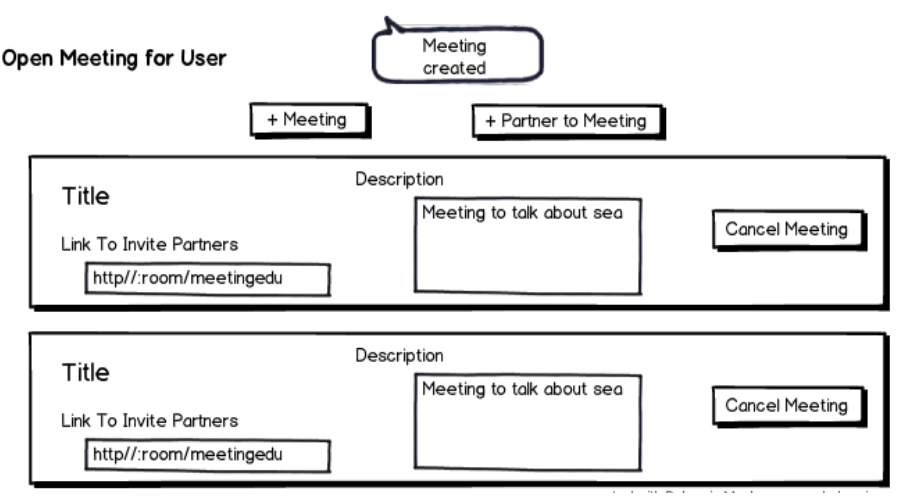
\includegraphics[scale=0.4]{Diseno/boceto}}

\caption{Maqueta de la primera versión}
\label{wrap:maqueta_1_version}
\end{figure}


En la figura \ref{wrap:maqueta_1_version} se observa lo esencial
de una funcionalidad para crear una nueva reunión (botón ``+ \emph{Meeting}'')
y un botón para agregar usuarios a la reunión (``+ \emph{Partner
to Meeting}'')\@. Aparecen los datos que se muestran para cada reunión,
tales como el título, un enlace para invitar usuarios ajenos a la
aplicación, una pequeña descripción y un botón para eliminar la reunión
(``Cancel Meeting'')\@. En la parte superior central se vislumbra
la idea de un mensaje superpuesto sobre la pantalla que alerta al
usuario que acaba de crear una reunión (``\emph{Meeting created}'')\@.
Este mensaje se desvanece progresivamente gracias a una funcionalidad
de \textit{jQuery UI} \cite{key-13}\@.

\begin{figure}[H]
\centerline{\includegraphics[scale=0.4]{Diseno/version_1}}

\caption{Primer interfaz de usuario visualizado en el explorador}
\label{interfaz1}
\end{figure}


A partir de la maqueta que observamos en la figura \ref{wrap:maqueta_1_version}
se ha implementado un interfaz elemental como el de la figura \ref{interfaz1},
para facilitar un avance más diligente\@. Se puede concluir que no
es muy atractivo, pero las funcionalidades más importantes, como el
enlace para invitar a otros usuarios o las URLs para usuarios ajenos a ``Campus do Mar''
se han implementado y agilizarán la evolución del interfaz y de las
funcionalidades finales\@. La necesidad de un interfaz más intuitivo
en términos generales era obvia\@. El enriquecimiento del estilo
también debía ocupar parte del tiempo para realizar un interfaz
elegante y afín al usuario final\@. Decisiones y tiempo después se
realizó un interfaz más atractivo y se empezó a evaluar la posibilidad
de un panel de control en la parte superior del interfaz disponible
en cualquier página de la aplicación que facilitase su navegación,
como se puede observar en la figura \ref{intefaz_final}\@. La presencia
de jQuery UI se hacía indispensable para abordar problemas complejos
de diseño y rematar la aplicación con un diseño sugerente\@. Todas
las ventanas emergentes y los efectos visuales que aparecen al presionar
los botones de la aplicación han sido diseñados utilizando jQuery
UI \cite{key-13}\@.

\begin{figure}[H]
\centerline{\includegraphics[scale=0.3]{\string"Fotos de eMeeting/meetingApp\string".png}}

\caption{Versión final del interfaz de usuario}
\label{intefaz_final}
\end{figure}


\smallskip{}



\subsection{Botonera para cada reunión\label{sub:Botonera-para-cada}}

Se describen a continuación las funciones de los botones que se contemplan
en la figura \ref{BotoneraParaCadaReuni=0000F3n}\@. En esta figura
se observa la botonera para administradores, como peculiaridad cabe
comentar la sutil diferencia entre la figura a) y la figura b) que
posee el botón para cambiar una reunión al estado mágica ya que este
menú es diferente para usuarios administradores\@.

\smallskip{}


\begin{figure}[H]
\hspace{3.5cm}\subfloat[Botonera para no administradores]{\includegraphics[scale=0.45]{\string"Fotos de eMeeting/Fotos antiguas/botonera_lateral_noAdmin\string".jpg}

}\hspace{1.5cm}\subfloat[Botonera para admi\-nistradores]{\includegraphics[scale=0.4]{\string"Fotos de eMeeting/Fotos antiguas/botonera_lateral_admin\string".jpg}

}

\caption{Botonera para cada reunión}


\label{BotoneraParaCadaReuni=0000F3n}
\end{figure}

\begin{itemize}
\item Join

Como se observa en la figura \ref{intefaz_final} el único botón verde
y el de mayor tamaño por su importancia permite el acceso a la sala
para disfrutar de la videoconferencia\@. Cuando el usuario pulse
este botón se abrirá un \emph{iframe} en el explorador que contendrá
la ventana de \textit{Adobe Connect}\textsuperscript{\textregistered{}}
con la URL que se haya configurado para esta sala\@. La URL de la
sala cambia en función del estado de la misma, lógica que se ha explicado
en la sección \ref{sec:Concepto-de-sala}\@.

\item Disabled

Deshabilita la sala temporalmente\@. Este botón sólo está disponible
para el dueño de la sala\@. Cuando se pincha en este botón se llama
a la función asociada y mediante el método POST se pasa una variable
\emph{booleana} en función de si la sala se encuentra habilitada o
deshabilitada para alternar su estado entre uno u otro\@.

\item Delete

Elimina la sala de la lista de reuniones disponibles en el interfaz
de usuario\@. Sin embargo, se ha decidido por diseño que una reunión
nunca se elimine por completo del sistema, es decir, se borra del
servidor \textit{Adobe Connect}\textsuperscript{\textregistered{}},
pero nunca de la base de datos de la aplicación de forma que en el
botón \textsl{\emph{A}}\emph{ll} \emph{Recordings} siempre estarán
disponibles las reuniones eliminadas con su correspondiente lista
de grabaciones si las hubiera\@.

\end{itemize}
\begin{figure}[H]
\centerline{\includegraphics[scale=0.25]{\string"Fotos de eMeeting/Minimized_rooms\string".png}}

\caption{Lista de reuniones reducida}


\label{ReduceMeeting}
\end{figure}

\begin{itemize}
\item Icono de flecha


Este icono situado a la derecha del botón Delete, ofrece la posibilidad
de minimizar el espacio que ocupa una reunión dentro del panel de control\@.
De esta forma el usuario puede observar más reuniones en la parte superior de la página, como se
puede observar en la figura \ref{BotoneraParaCadaReuni=0000F3n}\@.

\item Recordings


Proporciona el acceso a las grabaciones de la reunión\@. Las grabaciones aparecerán tras
esta ventana una vez hayan finalizado. En caso de que sea la reunión la que finalice
aparecerán, después de ejecutarse la correspondiente función en el
cron que se mencionó en la sección \ref{sec:CRON}, en la ventana emergente
que se despliega al pulsar en el botón \emph{All recordings}\@.

\item Change NickName


Ofrece la posibilidad de cambiar el nombre de usuario que aparecerá
en cada reunión de videoconferencia\@.

\item También se muestra un párrafo con información sobre la sala:

\begin{enumerate}
\item Fecha de creación de la sala\@.
\item Tipo de sala, ya sea pública o privada\@.
\item Número de usuarios de ``Campus do Mar'' invitados a la reunión\@.
\end{enumerate}
\end{itemize}
\begin{figure}
\centerline{\includegraphics[scale=0.4]{\string"Fotos de eMeeting/Fotos antiguas/eMeeting Final Help/TextoToInvite\string".png}}

\caption{Texto por defecto para invitar a usuarios a reuniones}


\label{InviteText}
\end{figure}

\begin{itemize}
\item Sobre \includegraphics[scale=0.6]{\string"Fotos de eMeeting/Fotos antiguas/eMeeting Final Help/miniatura_letter\string".png}


Al pulsar sobre este icono se despliega una ventana emergente como
la de la figura \ref{InviteText}\@. Se muestra un texto destinado
a usuarios ajenos a la aplicación de forma que si lo reciben puedan
disfrutar de la sala a partir de la URL que se incluye\@. El texto
contiene las instrucciones necesarias para entrar a la sala y la ventana
emergente un icono interrogante como el descrito a continuación con
las directrices necesarias para enviarlo\@.

\item Interrogante \includegraphics[scale=0.6]{\string"Fotos de eMeeting/Fotos antiguas/eMeeting Final Help/miniatura_question\string".png}


Este icono aparece a lo largo de la aplicación y con la ayuda de la
librería jQuery-tipTip emerge un mensaje al pasar el puntero por sobre él
que explica la funcionalidad del elemento al que acompaña, ver figura
\ref{EmergentHelp}\@.

\end{itemize}
\begin{figure}[H]
\centerline{\includegraphics[scale=0.4]{\string"Fotos de eMeeting/TipTipText\string".png}}

\caption{Mensaje emergente de ayuda}


\label{EmergentHelp}
\end{figure}

\begin{itemize}
\item Botón de recarga \includegraphics[scale=0.6]{\string"Fotos de eMeeting/Fotos antiguas/eMeeting Final Help/miniatura_reload\string".png}


Este icono ofrece la posibilidad de modificar los enlaces para invitar
a usuarios externos que se muestran en la figura \ref{InviteUsers}\@.
De esta forma puede invitarse a una lista de usuarios a una reunión
con estos enlaces y en el futuro invalidar esos enlaces para invitar
a otro grupo de usuarios de forma que los primeros no tendrán acceso
a la reunión a menos que se les envíe el nuevo enlace generado\@.

\item URLs para invitar a otros usuarios:

\begin{itemize}
\item Presenter Access


Este enlace proporciona a su poseedor privilegios de presentador en
la reunión, como se adelanta en la subsección \ref{sub:Definici=0000F3n-de-roles}\@.
Un presentador podrá introducir contenido en la sala, como presentaciones
o compartir su escritorio\@. Como es obvio podrá compartir la imagen de
su cámara web y el audio\@.

\item Limited Access


Por el contrario, este enlace otorga la posibilidad de disfrutar de
la reunión, pero no se podrá participar de forma activa en ella\@.
Tampoco tendrá la opción de compartir su cámara web o su audio\@.

\end{itemize}
\item Invite DigiMar Users


Se podrá invitar a una videoconferencia a usuarios ya registrados
en la aplicación, a partir de una lista generada con la técnica de
autocompletar\@. Para implementar esta ventana se ha empleado la
librería jQuery y la tecnología AJAX\@.

\end{itemize}
\begin{figure}
\centerline{\includegraphics[scale=0.5]{\string"Fotos de eMeeting/InviteUsers\string".jpg}}

\caption{Modos de invitación de usuarios a una reunión}


\label{InviteUsers}
\end{figure}


\medskip{}



\subsection{Botonera superior de menú\label{sub:Botonera-superior-de}}

Esta botonera situada en la parte superior del cuerpo central de la
web, como se puede ver en la figura \ref{MenuSuperior}, proporciona
el acceso a las funciones globales de la aplicación que se describen a continuación\@.

\begin{figure}[H]
\centerline{\includegraphics[scale=0.4]{\string"Fotos de eMeeting/Fotos antiguas/Botonera_superior\string".jpg}}

\caption{Menú superior}


\label{MenuSuperior}
\end{figure}


\medskip{}

\begin{itemize}
\item \emph{All Recordings}


\begin{figure}[H]
\centerline{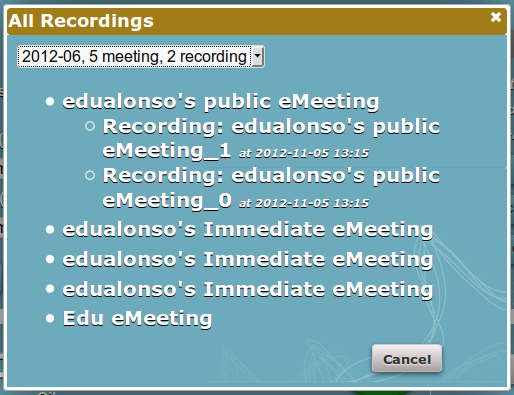
\includegraphics[scale=0.35]{Diseno/achievement_files}}

\caption{Ventana emergente para \textit{All recordings}}
\label{achievement_files}
\end{figure}
Desde este botón se accede a una lista de reuniones como la mostrada
en la figura \ref{achievement_files} que han finalizado\@. Ofrece
información sobre su fecha y hora de creación y la lista de grabaciones
en caso de existir\@.

\item \textit{Adobe Connect}\textsuperscript{\textregistered{}}\textsuperscript{}
\emph{Test}


\begin{figure}[H]
\centerline{\includegraphics[scale=0.4]{\string"Fotos de eMeeting/Fotos antiguas/adobe connect test\string".png}}

\caption{Prueba de conexión de \textit{Adobe Connect}\textsuperscript{\textregistered{}}\textsuperscript{}}


\label{TestAdobe}
\end{figure}



Se accede a una prueba de conexión facilitada por \textit{Adobe Connect}\textsuperscript{\textregistered{}}\textsuperscript{}
para ofrecer al usuario la seguridad de que existe conexión con el
servidor\@. Es un archivo Flash alojado en el servidor \textit{Adobe Connect}\textsuperscript{\textregistered{}},
que descarga un \textit{applet} en el navegador para realizar
las pruebas de conexión visualizándose un menú similar al de la figura
\ref{TestAdobe}\@.

\item \emph{eMeeting Help}


Al pinchar sobre este botón se accede a una ayuda que indica las diferentes
funciona\-lidades proporcionadas por eMeeting y explica cómo
se utilizan\@. Los usuarios podrán resolver las diferentes dudas
que puedan surgir sin más que ojear esta página\@. Ver figura \ref{HelpMeeting}

\item \emph{All eMeetings }


Este botón es realmente un filtro de reuniones por tipo. El nombre cambia
en función del filtro seleccionado ya sea público, privado, mágico, que sólo aparece si el usuario es administrador,
invitado para las reuniones a las que ha sido invitado el usuario y la opción marcada
por defecto, de ahí el nombre que vemos en la figura, que muestra
todas las reuniones del usuario\@. Este desplegable puede verse en
la figura \ref{FilterMeeting}, donde también puede observarse el
código de colores relacionado con cada tipo de reunión que aparece también a la izquierda de cada elemento reunión\@.

\end{itemize}
\begin{figure}
\centerline{\includegraphics[scale=0.4]{\string"Fotos de eMeeting/FilterMeeting\string".png}}

\caption{Desplegable para el filtro de reuniones}


\label{FilterMeeting}
\end{figure}

\begin{itemize}
\item Admin


Este botón sólo aparece en el menú de los administradores de la aplicación
y permite acceder a funcionalidades para actuar directamente sobre
la base de datos o visualizar las estadísticas de la aplicación en
tiempo real\@. Una de las funcionalidades a destacar es la posibilidad
de poder modificar el estado de las reuniones a pesar de no ser el
dueño\@. Ver figura \ref{AdminMenu}\@.

\item + eMeetings


En la ventana modal que se desplegará al pinchar sobre este botón
se podrá seleccionar el título de la reunión, el sobrenombre de usuario
que se visualizará en la sala, invitar usuarios de ``Campus do Mar''
a la nueva reunión y determinar el carácter de la sala (pública o
privada)\@. El campo descripción es opcional\@. Ver figura \ref{CreateMeeting}\@.

\end{itemize}
\begin{figure}
\centerline{\includegraphics[scale=0.4]{\string"Fotos de eMeeting/Fotos antiguas/creandoeMeetingpublico\string".png}}

\caption{Menú de creación de reuniones}


\label{CreateMeeting}
\end{figure}

\begin{itemize}
\item Change Password


Se accede a una ventana modal que permite cambiar la contraseña de
acceso a la aplicación.

\end{itemize}
\medskip{}



\subsection{Funciones PHP asociadas a la botonera}

En esta subsección se describirán las funciones relacionadas con los
botones que se han descrito en las secciones anteriores\@. De esta
forma se aclarará en detalle las comprobaciones y la lógica, transparente al usuario, que se realiza
en cada botón\@.

\smallskip{}

\begin{itemize}
\item Join


Este botón realiza una serie de comprobaciones antes de acceder a
la reunión co\-rrespondiente en \textit{Adobe Connect}\textsuperscript{\textregistered{}}\@.
\begin{itemize}
\item Comprueba el número de eMeetings simultáneos ya que está limitado
por las licencias compradas por el administrador del servidor de conexión
a \textit{Adobe}\textsuperscript{\textregistered{}}\@.
\item Comprueba que la sala todavía existe y que se tienen los privilegios necesarios
para disfrutar del eMeeting, ya que el usuario creador ha podido desahibilitar
la sala o incluso eliminarla antes de que la página se recargue y
por tanto todavía podría aparecer como activa en el interfaz\@.
\item Comprueba que el usuario posee los privilegios necesarios para acceder a
la reunión\@.
\end{itemize}

\item Enabled/Disabled


Con este botón el creador del eMeeting puede habilitar y deshabilitar
la sala a su voluntad impidiendo la entrada a todos los usuarios,
incluso aunque tengan acceso desde la puerta trasera creada en las
salas privadas, acceso descrito en la sección \ref{sec:Concepto-de-sala}\@.

\item Delete


Con este botón se elimina la sala del interfaz de usuario y también
de todos los usuarios invitados al eMeeting. Únicamente el creador
del eMeeting tiene el privilegio de eliminar su sala para evitar
futuros conflictos y potenciar que los usuarios creen sus propias
salas\@.


Antes de eliminar el eMeeting del interfaz se comprueba si posee grabaciones y se almacenan en una
carpeta interna de \textit{Adobe Connect}\textsuperscript{\textregistered{}}\@.
En el botón antes descrito como \emph{All recordings} se guarda el acceso
a las grabaciones de los eMeetings eliminados\@.

\item Recordings


Con este botón se visualizarán las grabaciones realizadas en el eMeeting
hasta el momento\@. Se accede vía AJAX al \emph{EndPoint} correspondiente
de Symfony para conseguir los valores actualizados de la lista de
grabaciones\@. En la sección \ref{sec:CRON} se ha hablado de la
función que se ejecuta en el servidor cada minuto para almacenar las
nuevas grabaciones en la base de datos al finalizar las mismas\@.

\item Change Nick Name


En la ventana modal que despliega este botón se da la opción de cambiar
el sobrenombre (\emph{NickName}) de cada reunión\@. Este código comprueba
que no se inserta un sobrenombre vacío, aunque sería posible en el
\textit{Adobe Connect}\textsuperscript{\textregistered{}}\textsuperscript{}
la posibilidad de no tenerlo\@.

\end{itemize}
\medskip{}



\section{URLs de acceso a la aplicación\label{sec:URLs-de-acceso}}

En esta sección, y para acompañar a las funcionaliadades descritas
en la sección \ref{sec:El-interfaz-de}, se explican con detalle las diferentes
rutas que se han implementado para esta aplicación y que dan acceso
a las funciones de los controladores\@. Symfony ofrece esta potente
funcionalidad de asociación entre URL y lógica a realizar al acceder
a dicha URL de acceso a la aplicación\@. A
raíz de la explicación de estas rutas de acceso en la sección \ref{sec:Concepto-de-sala}
el lector ya posee una visión más completa de la estructura de la
aplicación y también del gran trabajo que simplifica la utilización
de Symfony\@. En esta lista de rutas existen tres parámetros a destacar:

\begin{itemize}
\item El nombre para acceder a la función desde el interior de los controladores y plantillas.
\item Tipo de petición realizada sobre el servidor, ya ser POST o GET, para acceder a la función.
\item La URL para acceder a la función vía web.
\end{itemize}

\smallskip{}

Estos parámetros mejoran la seguridad de la aplicación ante ataques como la inyección SQL y ofrecen una fácil utilización de las funciones que describimos a continuación.

\smallskip{}

\begin{itemize}
\item index\_personal ANY /personal/


Esta función que se encuentra en el archivo \textit{Controller/PersonalController.php},
devuelve el usuario registrado, la lista de grupos a los que pertenece
el usuario, la lista de reuniones con estado NOW y la lista de reuniones
asociada a cada usuario con estado NOW que no pertenecen al grupo\@.

\end{itemize}
\smallskip{}

\begin{itemize}
\item group ANY /groupadmin/


Situado en \textit{Controller/GroupAdminController.php}, devuelve
una lista de todos los grupos que posee la aplicación\@.

\end{itemize}
\smallskip{}

\setcounter{footnote}{0}

\begin{itemize}
\item group\_show ANY /groupadmin/\{id\}\footnote{Los términos que aparecen entre llaves hacen referencia a la variable que se pasa mediante el método POST a cada una de las funciones.}/show


Situado en \textit{Controller/GroupAdminController.php}, recibe como
parámetro el identificador del grupo que se visualizará en el formulario
de edición para el menú de admi\-nistrador\@.

\end{itemize}
\smallskip{}

\begin{itemize}
\item group\_new ANY /groupadmin/new


Situado en \textit{Controller/GroupAdminController.php}, crea un
formulario para añadir un nuevo grupo en el menú de administrador\@.

\end{itemize}
\smallskip{}

\begin{itemize}
\item group\_create POST /groupadmin/create


Situado en \textit{Controller/GroupAdminController.php}, valida el
formulario creado en group\\
\_new y actualiza la base de datos\@.

\end{itemize}
\smallskip{}

\begin{itemize}
\item group\_edit ANY /groupadmin/\{id\}/edit


Situado en \textit{Controller/GroupAdminController.php}, recibe como
parámetro el identificador del grupo que se solicita editar en el
menú de administración\@.

\end{itemize}
\smallskip{}

\begin{itemize}
\item group\_update POST /groupadmin/\{id\}/update


Situado en \textit{Controller/GroupAdminController.php}, valida el
formulario de edición y actualiza la base de datos\@.

\end{itemize}
\smallskip{}

\begin{itemize}
\item group\_delete POST /groupadmin/\{id\}/delete


Situado en \textit{Controller/GroupAdminController.php}, borra un
grupo desde el menú de administrador actualizando la base de datos\@.

\end{itemize}
\smallskip{}

\begin{itemize}
\item meeting ANY /meeting/


Situado en \textit{Controller/MeetingController.php}, realiza una
consulta a la base de datos para mostrar al administrador una lista
con todas las reuniones de la aplicación\@.

\end{itemize}
\smallskip{}

\begin{itemize}
\item Las funciones meeting\_show ANY /meeting/\{id\}/show, meeting\_new
ANY /meeting/new, meeting\_create POST /meeting/create, meeting\_edit
ANY /meeting/\{id\}\-/edit, meeting\_update POST, /meeting/\{id\}/update,
meeting\_delete POST /mee\-ting/\{id\}/delete situadas en 
\textit{Controller/MeetingController.php}, son
análogas a las mencionadas en los párrafos anteriores para los grupos
y ofrecen al administrador las funcionalidades descritas y la validación
de los datos, para actuar sobre la base de datos, de una forma casi
instantánea para el programador\@.
\end{itemize}
\smallskip{}

\begin{itemize}
\item index\_welcome ANY /welcome 


Situada en \textit{Controller/SecurityController.php}, recibe la
dirección de correo electrónico que introduce el usuario al entrar
en la aplicación, la valida y si existe redirige al usuario a la pantalla
de entrada\@. También incluye el código que enviará un correo electrónico
de alerta a un usuario si se intenta acceder a su cuenta y se cumple
el máximo número de intentos de introducción de contraseña\@.

\end{itemize}
\smallskip{}

\begin{itemize}
\item mail\_sent ANY /mail/sent


Situada en \textit{Controller/SecurityController.php}, función que
envía el correo electrónico en caso de que un intruso intente acceder
a una cuenta de forma errónea\@.

\end{itemize}
\smallskip{}

\begin{itemize}
\item recover ANY /recover/\{email\}/\{hash\}


Situada en \textit{Controller/SecurityController.php}, si recibe
como parámetro POST una dirección de correo electrónico y una huella
(\textsl{hash}) asociada al usuario dueño del correo electrónico,
se cambiará la contraseña del usuario en la base de datos\@.

\end{itemize}
\smallskip{}

\begin{itemize}
\item recover\_error ANY /recover/error


Situada en \textit{Controller/SecurityController.php}, si la huella
que pasamos en la función anterior es incorrecta o la dirección de
correo electrónico no existe se supone un intento de ataque, para
defender a la aplicación de ello se redirige a esta función\@.

\end{itemize}
\smallskip{}

\begin{itemize}
\item recover\_update ANY /recover/update


Situada en \textit{Controller/SecurityController.php}, si la función
\textsl{recover} ha tenido éxito, se redirige a esta función que mostrará
un mensaje informando de que la contraseña se ha modificado correctamente\@.

\end{itemize}
\smallskip{}

\begin{itemize}
\item recording ANY /recording/


Situada en \textit{Controller/RecordingController.php}, devuelve
todas las grabaciones de la base de datos\@.

\end{itemize}
\smallskip{}

\begin{itemize}
\item Las funciones recording\_show ANY /recording/\{id\}/show, recording\_new
ANY /recor\-ding/new, recording\_create POST /recording/create, recording\_edit
ANY /recor\-ding/\{id\}/edit, recording\_update POST /recording/\{id\}/update,
recording\_delete POST /recording/\{id\}/delete 


Situadas en \textit{Controller/RecordingController.php}, de nuevo
ofrecen las mismas funcionalidades descritas para las reuniones y
para los grupos, en las cuales el admi\-nistrador puede actuar directamente
sobre la base de datos si fuese necesario\@.

\end{itemize}
\smallskip{}

\begin{itemize}
\item Para terminar con estas funciones específicas para el administrador
de la aplicación user ANY /useradmin/, user\_show ANY /useradmin/\{id\}/show,
user\_new ANY /useradmin/new, user\_create POST /useradmin/create,
user\_edit ANY /useradmin/\{id\}/edit, user\_update POST /useradmin/\{id\}/update,
user\_delete POST /useradmin/\{id\}/delete


Situadas en \textit{Controller/RecordingController.php}, también
realizan el tipo de operaciones relacionadas con la edición directa
de la base de datos por parte del admi\-nistrador\@.

\end{itemize}
\smallskip{}

\begin{itemize}
\item cmar\_meeting\_middleware\_index ANY /middleware


Ésta es la ruta de acceso a las funciones del \textsl{middleware}\@.
La llamada de ``Directorio +'', que se explicará con mayor detalle
en la sección \ref{sec:Directorio-+}, para recopilar o enviar datos
a la aplicación, invocará esta ruta para realizar diferentes funciones
tales como actualizar la aplicación o sincronizar servicios\@.

\end{itemize}
\smallskip{}

\begin{itemize}
\item index ANY /


Función situada en \textit{Controler/UserController.php}, envía la
información necesaria a la plantilla que visualiza el usuario al entrar
en la aplicación\@. Esta función hace una petición a la base de datos
para obtener todos los usuarios de la misma, la entidad con los datos
del usuario que realiza la petición, las reuniones que el usuario
posee activas y los sobrenombres que el propio usuario posee para
cada reunión\@. Esta función también contiene los datos de las funciones
futuras en caso de implementarse esta funcionalidad\@. Incluso se
ha implementado la lógica para mostrar las reuniones activas de otros
usuarios por si fuese de interés\@.

\end{itemize}
\smallskip{}

\begin{itemize}
\item index\_recording ANY /recording/\{id\}


Función situada en \textit{Controler/UserController.php}\@. Cuando
se invoca acompañada del identificador de una grabación comprueba
si la grabación está bloqueada devolviendo un mensaje con la información
o en caso contrario, redirigiendo al usuario al servidor \textit{Adobe Connect}\textsuperscript{\textregistered{}}\textsuperscript{}
para visualizar la grabación\@. Sólo un usuario registrado en la
aplicación podrá visualizar la grabación\@.

\end{itemize}
\smallskip{}

\begin{itemize}
\item index\_public\_recording ANY /recording\_public/\{id\}


Función situada en \textit{Controler/UserController.php}\@. Cuando
se invoca realiza comprobaciones similares a la función anterior pero
el usuario no precisa estar registrado en la aplicación\@. Característica
muy útil si se trabaja con usuarios ajenos a la aplicación\@.

\end{itemize}
\smallskip{}

\begin{itemize}
\item index\_immediate ANY /immediate


Función situada en \textit{Controler/UserController.php}, para crear
una nueva reunión en la base de datos\@. Se realizan las siguientes
comprobaciones antes de crear la reunión:
\begin{enumerate}
\item En caso de elegir la opción de sala mágica se comprueba si se ha llegado
al número máximo para este tipo de salas, en caso afirmativo se emite
un error\@.
\item Se comprueba si el estado de la sala está entre los posibles, para
evitar posibles ataques a la aplicación y obtener un error sobre la
base de datos\@.
\item Los títulos para las salas en \textit{Adobe Connect}\textsuperscript{\textregistered{}}\textsuperscript{}
no pueden exceder de 60 caracteres, por tanto se realiza esta comprobación
y si es necesario se da el error correspondiente\@.
\item Se comprueba si el título elegido existe en la aplicación ya que el
servidor \textit{Adobe Connect}\textsuperscript{\textregistered{}}\textsuperscript{}
no permite títulos duplicados\@.
\item Se procede a crear la sala en la base de datos y en el servidor \textit{Adobe Connect}\textsuperscript{\textregistered{}}\textsuperscript{},
para ello se invoca a la función \textit{createMeeting}\@. Esta
función se encuentra en el módulo de servicio para las reuniones en
\textit{Service/MeetingService.php}\@.
\item En caso de que todo sea correcto se muestra el mensaje de sala creada
correctamente y en caso contrario el mensaje: \textit{Error in ADO, you may need to change the title},
ya que es posible que el título elegido contenga algún caracter no
permitido\@.
\end{enumerate}
\end{itemize}
\smallskip{}

\begin{itemize}
\item change\_nickname ANY /changenick


Función situada en \textit{Controler/UserController.php}, que cambia
el nombre que un usuario mostrará en una reunión determinada\@. Esta
función comprueba que se introduce algún caracter y a continuación
si el nombre que se introduce no es el mismo que ya existe en la base
de datos para evitar modificaciones superfluas\@. Cabe mencionar
que por defecto este nombre de usuario para cada reunión, en caso
de que el usuario no especifique ninguno, será el nombre y apellidos\@.

\end{itemize}
\smallskip{}

\begin{itemize}
\item update\_rank ANY /updaterank


Función situada en \textit{Controler/UserController.php}, que ordena
la lista de reuniones que visualiza el usuario en su cuenta\@. En
el momento en el cual se accede a la aplicación y el usuario realiza
la consulta para obtener la lista de reuniones, se pide a la base
de datos que ordene esta lista según la varible \textit{rank}, perteneciente
a cada reunión\@. Esta variable \textit{rank} es la que actualiza
esta función\@. Esta actualización se realiza mediante una petición
AJAX para actualizar la base de datos\@. La animación de movimiento
de una reunión al pinchar sobre ella con el ratón se ha implementado
con la librería jQuery UI\@.

\end{itemize}
\smallskip{}

\begin{itemize}
\item addusers\_meeting ANY /addusers


Función situada en \textit{Controler/UserController.php}\@. Para
añadir usuarios a una reunión se pincha en el botón \textit{Invite DigiMar Partners}
y se despliega una ventana emergente en la cual se visualizan los
usuarios que ya han sido invitados a la reunión\@. Esta ventana invoca
a la función que se está describiendo, la cual realiza la petición
a la base de datos con la lista de usuarios para dicha reunión\@.
Esta ventana, mediante la técnica de autocompletado, ofrece una
lista de usuarios a partir de tres letras introducidas en el campo
de texto\@. La funcionalidad de autocompletado
realiza una petición AJAX para obtener los usuarios que coindicen
con las letras introducidas en dicho campo\@. Si se pincha
sobre un usuario, éste se añade a la caja de usuarios invitados a
la reunión\@. Si por el contrario pinchamos en el aspa a la derecha
de algún usuario invitado, éste será eliminado de la reunión\@. Las
operaciones realizadas sobre esta ventana emergente se confirmarán
pinchando en el botón \textit{Save}\@.


\begin{figure}[H]
\centerline{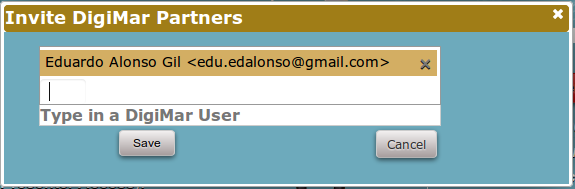
\includegraphics[scale=0.4]{Diseno/InviteDigiMarPartners}}

\caption{Ventana emergente al pinchar en el botón \textit{Invite DigiMar Partners}}
\end{figure}


\end{itemize}
\smallskip{}

\begin{itemize}
\item updateviewsalt\_meeting ANY /updateviewsalt/\{id\}, updatesecretsalt\_meeting
ANY /updatesecretsalt/\{id\}


Situadas en Controller/UserController.php, ambas rutas comparten la
misma función y en su interior se evalúa si el parámetro indicado
es \textsl{viewsalt} o \textsl{secretsalt}\@. Esta función ofrece
entrada a las reuniones con diferentes privilegios: si se envía \textsl{viewsalt}
los privilegios son limitados, acceso sólo para los que visualizarán
la reunión pero no podrán participar en ella; si se envía el \textsl{secretsalt}
se accederá a la reunión con privilegios de presentador\@.

\end{itemize}
\smallskip{}

\begin{itemize}
\item index\_cancel ANY /cancel/\{id\}


Situada en Controller/UserController.php, es la función que invoca
el botón \emph{Delete} de cada reunión\@. En esta función se comprueba
primeramente si la reunión ha finalizado ya, por si ocurriese algún
problema de sincronización, en caso contrario pasamos a cambiar el
estado de la reunión en la base de datos, lo cual eliminará la reunión
de la lista de reuniones en el índice de la aplicación del usuario\@.
Para ello se invoca a la función \textsl{stop} en el servicio de reuniones\@.

\end{itemize}
\smallskip{}

\begin{itemize}
\item index\_edit ANY /edit/\{id\}


Situada en Controller/UserController.php, despliega un formulario
para modificar una reunión existente, comprobando de inicio si el
usuario es el dueño de la reunión\@.

\end{itemize}
\smallskip{}

\begin{itemize}
\item index\_update POST /update/\{id\}


Situada en Controller/UserController.php, actualiza la base de datos
a partir de la información del formulario creado en \textsl{index\_edit}\@.

\end{itemize}
\smallskip{}

\begin{itemize}
\item index\_search\_meeting ANY /recordings/\{meeting\_id\}


Situada en Controller/UserController.php, crea una lista de grabaciones
de una reunión para mostrarla cuando se pincha en el botón \emph{All recordings}\@.

\end{itemize}
\smallskip{}

\begin{itemize}
\item index\_historical ANY /historical


Situada en Controller/UserController.php, genera la lista de reuniones
pasadas o eli\-minadas cuando se pincha en el botón \emph{All recordings}\@.

\end{itemize}
\smallskip{}

\begin{itemize}
\item index\_month ANY /historical/\{string\_month\}


Situada en Controller/UserController.php, ofrece la funcionalidad
de mostrar la lista de reuniones ordenadas por año y mes\@. Como
se puede ver en la ventana emergente de la figura \ref{RecordsUser}, al pinchar en el botón \emph{All recordings},
existe un menú para seleccionar año y mes, este menú
realiza una llamada a esta función para servir la lista de reuniones
correspondientes a esta fecha\@. También se puede ver que se muestra
el número de grabaciones para esa fecha, consulta realizada por esta
función para mostrarse en la ventana emergente\@.

\end{itemize}
\begin{figure}[H]
\centerline{\includegraphics[scale=0.3]{\string"Fotos de eMeeting/Fotos antiguas/achiement files\string".png}}

\caption{Lista de grabaciones de un usuario}


\label{RecordsUser}
\end{figure}


\smallskip{}

\begin{itemize}
\item change\_password ANY /change\_password/\{email\}


Situada en Controller/UserController.php, funcionalidad asociada al
botón \emph{Change Password} situado en el menú superior de la aplicación,
ver figura \ref{BotoneraParaCadaReuni=0000F3n}\@. Esta función busca
el usuario en la base de datos a partir de su dirección de correo
electrónico, para luego actualizar la base de datos con la contraseña
introducida en la ventana emergente\@. Si el método utilizado no
es POST se reporta un error ya que se ha detectado un intento de ataque
sobre esta función\@.

\end{itemize}
\smallskip{}

\begin{itemize}
\item recording\_list ANY /r\_list/\{id\}


Situada en Controller/UserController.php, está asociada a la petición
AJAX que realiza el botón \emph{Recordings} de cada reunión\@. Devuelve
el usuario dueño de la reunión y la entidad que representa la reunión\@.

\end{itemize}
\smallskip{}

\begin{itemize}
\item locked\_recording ANY /locked\_record/\{locked\}/\{id\}


Situada en Controller/UserController.php, bloquea las grabaciones
cuando pulsamos en el botón \emph{pausa}, ver figura \ref{RecordingUser},
asociado a cada grabación o la desbloquea en caso de que pulsemos
en dicho botón y la grabación esté bloqueada\@. Este botón realiza
una petición AJAX sobre esta función para que actualice el estado
de la entidad \emph{meeting} en la base de datos\@.

\end{itemize}
\smallskip{}


\begin{figure}
\centerline{\includegraphics[scale=0.3]{\string"Fotos de eMeeting/Fotos antiguas/recordings y URL\string".png}}

\caption{Menú de la lista de grabaciones de cada reunión}


\label{RecodingsMeetingAndState}
\end{figure}

\begin{itemize}
\item recording\_public\_list ANY /r\_public\_list/\{secretsalt\}


Situada en Controller/UserController.php, ofrece una lista de grabaciones
cuando se envía, a usuarios ajenos a la aplicación, la URL que aparece
en la parte superior de la ventana emergente que se despliega al pulsar
en el botón de grabaciones, como se ve en la figura \ref{RecodingsMeetingAndState}\@.
En la figura \ref{ExternalLinkRecordings} puede verse la lista de
grabaciones que visualizará el usuario que reciba la URL\@.

\end{itemize}
\smallskip{}


\begin{figure}
\centerline{\includegraphics[scale=0.3]{\string"Fotos de eMeeting/ListaRecordings\string".png}}

\caption{Lista de grabaciones para usuarios externos}


\label{ExternalLinkRecordings}
\end{figure}

\begin{itemize}
\item locked\_meeting ANY /locked/\{locked\}/\{id\}


Situada en Controller/UserController.php, bloquea las reuniones cuando
pulsamos en el botón \emph{Enabled/Disabled} asociado a cada reunión,
ver figura \ref{BotoneraParaCadaReuni=0000F3n}\@. Con tecnología
AJAX este botón cambia al estado deshabilitado (\textsl{disabled})
cuando la reunión está deshabilitada, de forma que si se pulsa, la
reunión se desbloquea\@. Este botón realiza una petición AJAX sobre
esta función para que actualice la base de datos\@.

\end{itemize}
\smallskip{}

\begin{itemize}
\item user\_form ANY /u\_form/\{id\}


Situada en Controller/UserController.php, devuelve los datos del usuario
indicado por el identificador que se le pasa mediate POST a la función
que genera el formulario para el menú de usuarios del administrador\@.
La plantilla generada puede verse en la figura \ref{UserAdminForm}\@.

\end{itemize}
\smallskip{}


\begin{figure}
\centerline{\includegraphics[scale=0.4]{\string"Fotos de eMeeting/EditUserForm\string".png}}

\caption{Plantilla para la edición de usuarios por el administrador}


\label{UserAdminForm}
\end{figure}

\begin{itemize}
\item user\_list ANY /u\_list


Situada en Controller/UserController.php, devuelve la lista de usuarios
coincidentes con las letras introducidas en el cajetín de búsqueda
de usuarios mediante una petición AJAX, cuando se quiere añadir nuevos
usuarios a una reunión\@.

\end{itemize}
\smallskip{}

\begin{itemize}
\item admin ANY /admin


Situada en Controller/UserController.php, consulta las tablas Log
y Log\_Total de la base de datos y envía los datos a la plantilla
que genera las tablas estadísticas, con el número de participantes
activos para cada reunión y totales, el tiempo de duración de las
reuniones activas, la fecha de inicio de la reunión, número de reuniones
activas, la fecha y hora de la consulta de la base de datos para completar
la tabla Log\_Total y el identificador único para la reunión dentro
del servidor \textit{Adobe Connect}\textsuperscript{\textregistered{}}\@.

\end{itemize}
\smallskip{}

\begin{itemize}
\item indexgroup ANY /group/\{key\}


Situada en Controller/GroupController.php, comprueba que existe el
grupo solicitado, a continuación comprueba que el usuario que solicita
la información pertenece al grupo y finalmente devuelve a la plantilla
las reuniones actuales, las reuniones programadas y la entidad que
describe las características del grupo\@.

\end{itemize}
\smallskip{}

\begin{itemize}
\item indexgroup\_recording ANY /group/recording/\{id\}


Situada en Controller/GroupController.php, redirige a la grabación
del grupo solicitada\@.

\end{itemize}
\smallskip{}

\begin{itemize}
\item indexgroup\_immediate ANY /group/immediate/\{key\}


Situada en Controller/GroupController.php, construye una reunión para
un grupo determinado de manera que todos los componentes del grupo
serán invitados a la reunión creada\@.

\end{itemize}
\smallskip{}

\begin{itemize}
\item indexgroup\_cancel ANY /group/cancel/\{id\}


Situada en Controller/GroupController.php, actualiza el estado de
una reunión a \textit{CANCELLED} con lo cual ya no aparece en la
lista de reuniones para los usuarios pertenecientes al grupo y pasa
a formar parte de la lista de \textit{All recordings}\@.

\end{itemize}
\smallskip{}

\begin{itemize}
\item indexgroup\_delete ANY /group/delete/\{id\}


Situada en Controller/GroupController.php, elimina la reunión de la
base de datos\@. Esta función no se utiliza en la versión final ya
que se ha preferido mantener la información de todas las reuniones
en la base de datos y únicamente actualizar su estado para poder acceder
a información de reuniones borradas si fuese necesario\@.

\end{itemize}
\smallskip{}

\begin{itemize}
\item indexgroup\_edit ANY /group/edit/\{id\}


Situada en Controller/GroupController.php, crea el formulario necesario
para editar información a cerca de una reunión de grupo ya creada\@.

\end{itemize}
\smallskip{}

\begin{itemize}
\item indexgroup\_update POST /group/update/\{id\}


Situada en Controller/GroupController.php, la información de la reunión
descrita en el formulario creado en la función anterior se valida
en esta función y se actualiza en la base de datos\@.

\end{itemize}
\smallskip{}

\begin{itemize}
\item indexgroup\_historical ANY /group/historical/\{key\}


Situada en Controller/GroupController.php, crea una lista con las
reuniones de un grupo que ya han finalizado y poseen el estado \textit{CANCELLED}\@.

\end{itemize}
\smallskip{}

\begin{itemize}
\item indexgroup\_month ANY /group/historical/\{key\}/\{string\_month\}


Situada en Controller/GroupController.php, devuelve la lista de reuniones
de grupos con sus respectivas grabaciones\@. La petición se hace
para un mes y año concretos, de forma similar a \textit{All recordings}
para las reuniones de usuarios individuales\@. A la vez que se visualiza
el número de reuniones para un mes en la lista desplegable, también
se puede saber el número de grabaciones en ese mes\@.

\end{itemize}
\smallskip{}

\begin{itemize}
\item index\_room ANY /room/\{salt\}, index\_secretroom ANY /secretroom/\{salt\},
index\_\\
noanonymousroom ANY /noanonymousroom/\{salt\}, index\_noanonymoussecretroom
ANY /noanonymoussecretroom/\{salt\}


Situadas en Controller/RoomController.php, todas estas URLs llaman
a la misma función\@. Implementa un control de acceso a las reuniones
a partir de una URL secreta generada con el algoritmo MD5 a partir
del nombre de la reunión y otros datos, a parte de una huella aleatoria\@.
El usuario que posea la URL podrá acceder a la reunión con unos privilegios
determinados en función de si la URL que posee contiene el parámetro
\textsl{salt}, \textsl{secretsalt} o \textsl{viewsalt} de la reunión\@.
Para dar acceso a una reunión se comprueba ese parámetro de la URL
y el estado de la reunión, de forma que el usuario que accede a la
misma podrá ser presentador o asistente\@. El acceso también podrá
ser anónimo, es decir, un usuario que no tenga una cuenta en la aplicación
también tendrá acceso a través de las URLs que no contienen \textit{noanonymousroom}
o \textit{noanonymoussecretroom}\@. Estas URLs no redirigen a sus
correspondientes plantillas para entrada de acceso anónimo o para
que accedamos a un menú de registro en la aplicación\@. De esta forma
la aplicación siempre tendrá el control sobre los usuarios que acceden,
pertenezcan o no a la lista de usuarios registrados en la aplicación\@.
Para obtener control total de los privilegios de acceso de usuarios
anónimos, no registrados en la aplicación, se crea un usuario temporal
en el servidor \textit{Adobe Connect}\textsuperscript{\textregistered{}},
que luego será eliminado desde la función del cron correspondiente
como se ha explicado en la sección \ref{sec:CRON}\@.

\end{itemize}
\smallskip{}

\begin{itemize}
\item login ANY /login


Esta ruta redirige a la plantilla de entrada a la aplicación, si se
accede a una ruta configurada como privada en el archivo \textit{security.yml}\@.
Es una ruta por defecto que ofrece el \textit{framework} Symfony
para simplificar el intercambio entre mecanismos de registro en aplicaciones
y para simplificar el acceso de usuarios anónimos a la aplicación\@.
Esta ruta, al igual que las dos que se describen a continuación,
se encuentran en el fichero \textit{routing.yml}\@. Ofrece un
formulario para acceder a través del correo electrónico del usuario
y su contraseña asociada, además de un enlace a un formulario de recuperación
de contraseña\@. Para mayor seguridad el formulario de recuperación
de contraseña envía un correo electrónico a la cuenta indicada y se
genera un enlace único enviado a ese correo electrónico que redirige
a un nuevo formulario para cambiar la contraseña directamente en la
base de datos\@.

\end{itemize}
\smallskip{}

\begin{itemize}
\item login\_check ANY /


Esta ruta que pertenece al fichero \textit{routing.yml} controlará
el envío de formularios de inicio de sesión\@. Es decir todo usuario
que intente acceder a la aplicación será reenviado a la función loginAction
del archivo Controller/SecurityController.php\@. En este archivo
se evaluará el resto de la URL de acceso para comprobar qué tipo de
acceso se está llevando a cabo de los definidos en el archivo \textit{security.yml}\@.

\end{itemize}
\smallskip{}

\begin{itemize}
\item logout ANY /logout


Esta función perteneciente al fichero \textit{routing.yml} realiza
la salida de la aplicación\@. Es una función interna a la lógica
de Symfony, al igual que las dos anteriores y ofrece potentes mecanismos
de seguridad\@.

\end{itemize}
\medskip{}



\section{Interfaz de \textit{Adobe Connect}\textsuperscript{\textregistered{}}}

En esta sección se describe el interfaz de \textit{Adobe Connect Professional}\textsuperscript{\textregistered{}}
al que se accede al pinchar en el botón \textit{Join} de la aplicación\@.
Como ya se ha comentado en la sección \ref{sec:AdobeConnectProfessional}
y se puede observar en la figura \ref{AdobeInterface} el interfaz
de videoconferencia lo ofrece \textit{Adobe Connect Professional}\textsuperscript{\textregistered{}},
de todas formas este interfaz posee varios modos que pueden ser configurados
desde la aplicación eMeeting\@. En cada uno de estos modos
la disposición de los elementos de la pantalla cambia para ofrecer
interfaces apropiados a cada uso, como puede ser una videoconferencia
múltiple, una ponencia con presentaciones de diapositivas o reuniones
colaborativas donde las herramientas de intervención son más accesibles\@.
En la figura se observan las funcionalidades que ofrece \textit{Adobe Connect Professional}\textsuperscript{\textregistered{}} tales como un chat, la lista de usuarios con sus roles,
el menú para actuar sobre la reunión y poder grabarla o finalizarla,
los diferentes diseños para la plantilla o la posibilidad de grabar
el audio, escuchar otros audios o incluso compartirlos en la videoconferencia\@.

\begin{figure}
\centerline{\includegraphics[scale=0.4]{\string"Fotos de eMeeting/ADOInterface\string".png}}

\caption{Interfaz de videoconferencia de \textit{Adobe Connect}\textsuperscript{\textregistered{}}}


\label{AdobeInterface}
\end{figure}



\section{Directorio +\label{sec:Directorio-+}}

Es un servidor que almacena los datos de todas las aplicaciones y ofrece
un servicio de sincronización e información\@. Comercialmente recibe
el nombre de ``Directorio +'' y proveerá a todas las aplicaciones
de ``Campus do Mar'' de información para cargar sus bases de datos,
tales como usuarios y sus datos personales, pertenencia a determinados
grupos, contraseñas y otros datos de interés. Es la parte más compleja
del sistema ya que en combinación con el servidor CAS, que se explicará
en la sección \ref{sec:Seguridad-de-la} y ofrecerá un servicio de
autenticación, permitirá registrarse a todos los usuarios en todas
las aplicaciones desde el momento en que se registre en una de ellas\@. La información
modificada en cualquier aplicación se sincronizará con el resto gracias
al ``Directorio +''\@. Este servidor realizará peticiones periódicas
a todas las aplicaciones, incluida eMeeting, para actualizar
datos\@. Este flujo de datos se realizará en ambos sentidos y con
un formato determinado\@. La descripción de los datos solicitados
se almacena en archivos XML y ``Directorio +'' ejecutará las funciones
que necesite para actualizarse adecuadamente\@. La descripción de
las funciones que ejecutará Directorio + referentes a eMeeting se
almacenan en un fichero llamado \texttt{middleware.wsdl} y que ambas
partes poseen\@. Evidentemente el archivo de eMeeting sólo
contiene las funciones de sincronización propias que se describen a continuación\@.

\medskip{}



\subsection{El Middleware\label{sub:El-Middleware}}

\textsl{Middleware}, es un término utilizado para referirse al \emph{software}
que media para conectar dos entidades \emph{software} en un sistema
distribuido\@.

\smallskip{}


En el fichero \texttt{middleware.wsdl} se indica el formato de información
que ``Directorio +'' envía a eMeeting en formato XML\@. Esta
información se procesará en las distintas funciones implementadas
en la aplicación para rellenar los campos necesarios en la base de datos,
para los usuarios y grupos pertenecientes a la plataforma ``Campus
do Mar''\@. Algunas de estas funciones son: \textit{createUser, EnjoinGroup o addGroup}\@.
Cada una de estas funciones, a partir de los flujos generados por
``Directorio +'' hacia la aplicación, adaptan los datos enviados
para almacenarlos en la base de datos, de esta forma se realiza la
sincronización de la aplicación eMeeting de forma completamente
transparente para el usuario\@. La primera función añade un nuevo
usuario a la aplicación cuando un nuevo usuario es añadido a ``Directorio
+''\@. Si un nuevo usuario es añadido a un grupo se invoca la segunda
función y en caso de crear un nuevo grupo se invocará la tercera función\@.

\medskip{}



\section{Seguridad de la Aplicación\label{sec:Seguridad-de-la}}

En el fichero \texttt{security.yml} de Symfony se han configurado
tres opciones de registro para la aplicación\@. La ofrecida por HTML
con un desplegable donde se puede introducir login y contraseña, el
método de configuración de servidores de control de acceso (entidades
certificadoras) o la que ofrece Symfony mediante la redirección a
un formulario que se puede adaptar a las necesidades del administrador como puerta de
acceso a la aplicación\@.

\smallskip{}


De esta forma es posible alternar fácilmente entre tres tipos de registro
sin más que comentar y descomentar unas cuantas líneas en el fichero
\texttt{security.yml}\@.

\smallskip{}


Como aplicación independiente descrita en el capítulo \ref{chap:Dise=0000F1o-del-proyecto},
es imprescindible que eMeeting ofrezca estos diferentes tipos
de seguridad y registro de usuarios\@. Una de las más interesantes
es la posibilidad de registrarse a través de un servidor CAS, que
pasamos a describir\@.

\begin{table}[H]
\centerline{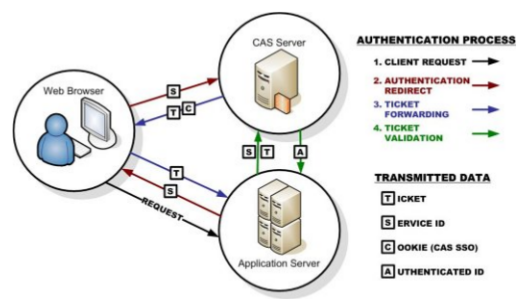
\includegraphics[width=12cm,height=7cm]{Diseno/CAS}}

\caption{Servidor CAS}
\label{Servidor_CAS}
\end{table}


CAS (\foreignlanguage{english}{\textsl{Central Authentication Service}})
es una aplicación web que permite implementar el conocido SSO (\foreignlanguage{english}{\textsl{Single
Sign On}}), un procedimiento de autenticación que habilita a un usuario
para acceder a distintas aplicaciones web (en distintos dominios y
en distintos servidores) únicamente registrándose una vez\@. En la
figura \ref{Servidor_CAS} se describe el intercambio de paquetes entre
las entidades que realizan el registro\@. En general, cuando un usuario
se conecta a una de las aplicaciones involucradas en el sistema se comprueba
si está autenticado y si no lo está lo redirige a la pantalla del
servidor de autenticación. Si el proceso finaliza correctamente el sistema
de autenticación, en este caso CAS, vuelve a redirigir al usuario
a la página que se solicitaba en un primer momento. El desarrollador
no tiene que preocuparse por mantener la seguridad y tener un formulario
de login en cada una de las aplicaciones web que desarrolla, sino
que simplemente se comprueba de si el usuario ya está
registrado, que es tan sencillo como efectuar una petición request
de esta forma: \texttt{request.getRemoteUser}\@. Si el método devuelve
null es que no está registrado y será redireccionado a la página de
login de CAS\@. Si ya está registrado por CAS, este método devolverá
un valor con el que sabremos que es un usuario registrado\@. Algo
que debe quedar muy claro es que CAS se encarga única y exclusivamente
de la autenticación, es decir, de comprobar contra una fuente de datos
específica si el usuario y contraseña facilitados existen y son correctos.
No se encarga de la autorización, que sería la gestión de lo que puede
o no puede hacer ese usuario en función de sus roles\@.

\smallskip{}


\begin{figure}
\subfloat[Formulario de registro en el servidor CAS]{\centerline{\includegraphics[scale=0.3]{\string"Fotos de eMeeting/CASService\string".png}}

\label{LoginFormCAS}}

\hspace{5cm}\subfloat[Formulario de acceso con diseño ``Campus do Mar'']{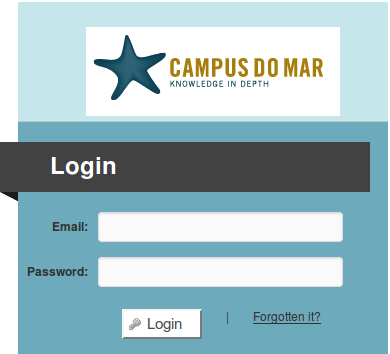
\includegraphics[scale=0.35]{Diseno/login}\hspace{0.8cm}



\label{loginDigiMarForm}}

\subfloat[Formulario básico que ofrece HTML]{\hspace{3cm}\includegraphics[scale=0.3]{\string"Fotos de eMeeting/BasicFormAutentication\string".png}

\hspace{3cm}

\label{loginBasicForm}}

\caption{Formularios de registro}
\end{figure}


En el servicio desplegado en ``Campus do Mar''el control de
acceso se realiza mediante dicho servidor CAS, implementado para todas las aplicaciones
de ``Campus do Mar'' introduciendo usuario y contraseña en el formulario
de la figura \ref{LoginFormCAS}\@.

\smallskip{}


Como se ha comentado para eMeeting también se ha implementado
la posibilidad de acceder a través de un formulario creado con Symfony\@.
Symfony compara la información introducida con la almacenada en la
base de datos de la aplicación, para permitir el acceso a la aplicación\@.
Como se observa en la figura \ref{loginDigiMarForm}, el acceso es
sencillo y posee un enlace para recuperar la contraseña en caso de
que el usuario la olvide\@.

\smallskip{}


Por último se ha implementado la opción de registro que ofrece HTML
con un formulario sencillo que accede a la base de datos para comprobar
que el usuario y contraseña introducidos son correctos como se muestra
en la figura \ref{loginBasicForm}\@.

\smallskip{}


El fichero \textit{routing.yml} es el único que se debe modificar
para alternar entre todas las posibilidades de acceso implementadas\@.
Cabe resaltar que incluso se puede definir el tipo de acceso para
cada una de las rutas descritas en la sección \ref{sec:URLs-de-acceso}\@.
La parte útil de este hecho reside en poder definir qué partes de
la aplicación, denominadas públicas, sean accesibles por usuarios
no registrados en la aplicación, como por ejemplo, las grabaciones
de las reuniones\@. Para el acceso a las zonas públicas se ha implementado
un control de acceso manejado por el usuario\@.

\medskip{}



\section{Comandos para una gestión de mayor comodidad}

En esta sección se describen una lista de comandos creados para gestionar
diferentes parámetros de la aplicación\@. Uno de los usos más importantes
de estos comandos es la posibilidad de ejecutarse a través de un cron
o \textit{bot} en el servidor para realizar tareas automatizadas de
mantenimiento o extraer estadísticas\@.

\smallskip{}

\begin{itemize}
\item Importación de usuarios definida en la base de datos interna de la
aplicación


La aplicación posee una base de datos interna que carga una serie
de usuarios por defecto definidos en el corazón de la aplicación que
facilita el testeo de la aplicación, y sus respectivas pruebas en
un nuevo servidor a la hora del despliegue\@. En el fichero \textit{DataFixtures/ORM/LoadUserData.php}
se crean los usuarios que serán introducidos por defecto en la base
de datos cuando se ejecute el comando \texttt{cmar:import:user}\@.
Esta lista de usuarios suele tener privilegios de administrador para probar
todas las funciones displonibles\@.

\item Estado de las reuniones


El comando \texttt{cmar:meeting:cron} permite conocer el estado de
las reuniones y probar las últimas funcionalidades de manera ágil
y rápida, como se ha explicado en la sección \ref{sec:CRON}\@.

\item Comprobación de la sincronización de usuarios


El comando \texttt{cmar:sync:user}, ofrece la posibilidad de comprobar
si los usuarios de la base de datos interna de la aplicación existen
en el servidor de \textit{Adobe Connect}\textsuperscript{\textregistered{}}\textsuperscript{}\@.
En caso contrario los usuarios no podrán disfrutar de videoconferencias
dentro de la aplicación como usuarios internos\@.

\item Comprobación de conectividad con el servidor de \textit{Adobe Connect}\textsuperscript{\textregistered{}}\textsuperscript{}


El comando \texttt{cmar:test:meeting}, permite comprobar si el servidor
donde se aloja la aplicación eMeeting posee conectividad con
el servidor donde está alojada la aplicación \textit{Adobe Connect}\textsuperscript{\textregistered{}}\textsuperscript{}\@.
Una forma rápida de detectar errores de conexión con dicho servidor
ayudará a descartar errores ágilmente\@.

\end{itemize}
\medskip{}



\section{Servicios de la aplicación}

Los servicios se describen en el fichero de configuración \textit{Resources/config/services.xml}\@.
En este fichero se encuentra la configuración del tipo de dato de
entrada para cada servicio de la aplicación\@. Este fichero en formato
XML guarda en sus variables los datos de conexión al servidor \textit{Adobe Connect}\textsuperscript{\textregistered{}}\@.
Las variables almacenadas son la URL donde está alojado el servidor
\textit{Adobe Connect}\textsuperscript{\textregistered{}}con los
datos de registro del usuario administrador, ya que es necesario para
utilizar todas las opciones de la API\@. También se encuentran aquí
los datos que limitan el uso del servidor como son el número total
de salas contratadas\@. Se define aquí también el número de salas
mágicas y por tanto también el número de salas que serán de libre
acceso para cualquier usuario, de esta forma si se desea modificar
este número sólo debe cambiar este archivo\@. Como ya se ha comentado,
dentro del servidor existe una carpeta en la que se almacenarán todas
las grabaciones de las reuniones que los usuarios borren\@. El identificador
de esta carpeta que será permanente durante la vida de cada aplicación,
se configurará también en este archivo\@.

\smallskip{}


Se describen a continuación los servicios de la aplicación y los parámetros
relativos a cada servicio\@.

\smallskip{}

\begin{itemize}
\item Servicio de Meeting


Este servicio recibe como parámetros desde el fichero \textit{services.xml}
el identificador de Doctrine, usado para el acceso a la base de datos
y el identificador del servicio AdoAdmin, debido a que se usarán gran
cantidad de las funciones que se crean en este fichero para acceder
al servidor \textit{Adobe Connect}\textsuperscript{\textregistered{}}\@.
Se le envía el número total de salas disponibles, o lo que es lo mismo,
el máximo número de licencias de \textit{Adobe Connect}\textsuperscript{\textregistered{}}
disponibles, el número de salas simultáneas y el número de salas mágicas\@.
Por último también se envía el identificador del servicio de registro
ya que es necesario que estas funciones se encuentren disponibles
para posibles accesos a las salas y al interfaz de usuario\@. El
servicio de registro permite obtener los datos del usuario que accede
a la aplicación y poder así ofrecerle sus parámetros y los privilegios
que posee dentro de la aplicación\@.


En este servicio se proporcionan a la aplicación las funciones para
actuar sobre las reuniones de la aplicación y acceder a funciones
de la API de \textit{Adobe Connect}\textsuperscript{\textregistered{}}\@.
\begin{itemize}
\item Función para crear reuniones en la base de datos de la aplicación


En este servicio se aloja la función que crea las reuniones en la
base de datos de la aplicación\@. Recoge los datos que le ofrece
el formulario de creación de reuniones de la aplicación como el título,
el usuario que la crea, el sobrenombre (\textit{nickname}) que ese
usuario desee mostrar para esta reunión en concreto, por defecto su
nombre y apellidos, un parámetro que indica si la sala es pública
o privada, una pequeña descripción de la reunión si se desea, y para
los usuarios administradores también aparece la opción de elegir si
la sala será mágica o no como se ha descrito en la subsección \ref{sub:Sala-m=0000E1gica}\@.

\item Función para crear reuniones en el servidor \textit{Adobe Connect}\textsuperscript{\textregistered{}}\textsuperscript{}


En este servicio se aloja la función que crea las reuniones en el
servidor \textit{Adobe Connect}\textsuperscript{\textregistered{}}\textsuperscript{}\@.
Cuando se pulsa el botón ``Join'' de la aplicación se ejecuta esta
función que mediante el uso del servicio administrador de \textit{Adobe Connect}\textsuperscript{\textregistered{}}\textsuperscript{}
crea la reunión en el servidor e introduce al usuario en la sala\@.
También se cambia el estado de la sala y se almacena en la base de
datos la URL que, para \textit{Adobe Connect}\textsuperscript{\textregistered{}}\textsuperscript{},
identificará esta sala\@.

\item Función para eliminar reuniones en el servidor \textit{Adobe Connect}\textsuperscript{\textregistered{}}\textsuperscript{}


En esta función se hace una búsqueda de la reunión en la base de datos
de \textit{Adobe Connect}\textsuperscript{\textregistered{}}\textsuperscript{}
mediante la URL que identifica la sala\@.
Una vez identificada la reunión se procede a guardar sus grabaciones,
si las hubiese, en una carpeta alojada en el servidor \textit{Adobe Connect}\textsuperscript{\textregistered{}}\textsuperscript{} que
se ha creado específicamente para este fin\@. Acto seguido se cambia
el estado de la reunión en la base de datos de la aplicación a finalizada\@.

\item Función para añadir usuarios de ``Campus do Mar'' a reuniones en
el servidor \textit{Adobe Connect}\textsuperscript{\textregistered{}}


Esta función recibe como parámetros la entidad \emph{meeting} y una
lista con los usua\-rios que debe contener la reunión, por tanto, se
eliminan todos los usuarios de la reunión menos el creador y se añaden
todos los usuarios que contiene la lista recibida. Debido a que es
posible que un usuario quiera borrar únicamente al propietario de
la reunión y no al resto se añade una comprobación en la cual si en
la lista recibida no está el propietario de la reunión, se devuelve
un error y no se modifica la lista de usuarios\@.

\item Función para crear usuarios en el servidor \textit{Adobe Connect}\textsuperscript{\textregistered{}}\textsuperscript{}


Esta función recibe todos los campos necesarios para crear un usuario
en el servidor \textit{Adobe Connect}\textsuperscript{\textregistered{}}\textsuperscript{},
login, nombre, apellidos, correo electrónico, descripción y contraseña\@.
Estos datos se introducen en el servidor con la llamada \texttt{principal-up\-date}
de la API de \textit{Adobe Connect}\textsuperscript{\textregistered{}}\@.

\item Control de acceso a las reuniones en el servidor \textit{Adobe Connect}\textsuperscript{\textregistered{}}\textsuperscript{}


Esta función devuelve verdadero o falso tras realizar una serie de
comprobaciones que indican si está permitido el acceso a una determinada
reunión, comprobando si el usuario está en la base de datos o es un
usuario anónimo, si la reunión está bloqueada, si el usuario pertenece
a la lista de invitados o es el creador, y si, en caso de ser un usuario
anónimo, accede desde la URL correspondiente como se ha descrito en
la sección \ref{sec:URLs-de-acceso}\@.

\item Función para cambiar el sobrenombre (\textit{nickname}) de usuario


La aplicación permite tener un nombre corto para cada reunión\@.
De esta forma en la actual función se implementa una lógica que permite
modificar el nombre corto asociado a cada usuario en cada reunión\@.

\item Función para cambiar la huella (\emph{``hash}'') de la entrada secreta


En esta función se implementa un cambio aleatorio de una clave que
permite entrar a una sala con ciertos privilegios otorgados por el
creador de la reunión\@. Podría decirse que
es una llave maestra que otorga el creador de la sala para poder entrar
en ella, en ocasiones con los mismo privilegios que el creador\@.
Esta función en concreto implementa la lógica que permite modificar
dicha llave maestra para que los usuarios que tengan una llave maestra
obsoleta ya no puedan disfrutar de la sala y se les tenga que enviar
la nueva llave otra vez\@.

\item Función para cambiar la huella de la entrada común


Al igual que para la entrada secreta también se crea una huella
para la entrada común con el algoritmo MD5 que permite el acceso con
privilegios de presentador a la sala e identifica cada reunión\@.

\item Función para cambiar la contraseña de usuario


En esta función se implementa una llamada a la API de \textit{Adobe Connect}\textsuperscript{\textregistered{}}\textsuperscript{}
para cambiar la contraseña de usuario en dicho servidor, ya que las
contraseñas de los usuarios deben estar sincronizadas entre el servidor
\textit{Adobe Connect}\textsuperscript{\textregistered{}}\textsuperscript{}
y el servidor de la aplicación\@.

\end{itemize}
\end{itemize}
\medskip{}

\begin{itemize}
\item Servicio de aplicación de \textit{Adobe Connect}\textsuperscript{\textregistered{}}


En este servicio se implementan dos funciones que relacionan de forma
directa la aplicación con el servidor \textit{Adobe Connect}\textsuperscript{\textregistered{}}\@.
Una obtiene los datos para registrarse con privilegios de administrador
y poder controlar la API y la otra crea usuarios nuevos en el servidor
dando las credenciales oportunas\@.

\item Servidor


Esta función obtiene las credenciales del servidor donde se aloja
la aplicación \textit{Adobe Connect}\textsuperscript{\textregistered{}}\@.
\begin{itemize}
\item Cookies


Se refiere a diferentes funciones que guardan y rescatan la cookie
de sesión que el servidor \textit{Adobe} ofrece cada vez que se realiza
un entrada en la aplicación\@.

\item Función de login


Esta función realiza el registro en el servidor \textit{Adobe} con
las credenciales del usuario que realiza la petición desde la aplicación\@.
Realiza una serie de peticiones utilizando la función curl \cite{key-4}
accediendo a la API de \textit{Adobe} para procesar las respuestas
del servidor y determinar si la operación se ha realizado con éxito\@.
Se han di\-señado una serie de excepciones para determinar posibles
errores en el registro y atarjarlos ágilmente\@.

\end{itemize}
\item Servicio de administrador de \textit{Adobe Connect}\textsuperscript{\textregistered{}}\textsuperscript{} (\textit{AdoAdmin})


Desde el archivo \textit{services.xml} se envía la URL donde se aloja
el servidor \textit{Adobe Co\-nnect}\textsuperscript{\textregistered{}},
el usuario y contraseña de acceso para el usuario administrador, la
carpeta donde se alojarán las grabaciones cuando se elimina una sala
y el servicio de registro\@.


Este servicio alberga los comandos de la API de \textit{Adobe Connect}\textsuperscript{\textregistered{}}
para realizar las diferentes acciones sobre el servidor\@. Algunas
de estas acciones son la creación de usuarios, la creación de reuniones,
el cambio de contraseña para un usuario o la ac\-tualización de cualquiera
de las entidades que alberga el servidor \textit{Adobe}\@.

\item Factoría de Adobe


Proporciona funciones para utilizar la
API de \textit{Adobe Connect}\textsuperscript{\textregistered{}}\textsuperscript{}\@.
Desde este servicio se obtiene el nombre del servidor donde se aloja
\textit{Adobe Connect}\textsuperscript{\textregistered{}}\textsuperscript{}
necesario para la comunicación entre ambas aplicaciones\@. Para ello se inyecta el
archivo \textit{services.xml} que posee las variables tales como la URL de acceso
al servidor y el servicio de registro para utilizarlos en esta función\@. También
se obtiene el usuario que está conectado en ese momento y otorga la
capacidad de hacer una llamada a la administración de \textit{Adobe}
para crear un usuario en caso de que no se encuentre registrado en
el servidor\@.

\item Interfaz de administración para \textit{Adobe Connect}\textsuperscript{\textregistered{}}\textsuperscript{}


En el interfaz de administración deben añadirse las cabeceras de las
funciones más importantes de la aplicación como son crear y borrar
reuniones\@.

\item Servicio de Mail


Este servicio permite utilizar las herramientas de Symfony para enviar
correos tanto a los usuarios como a los administradores\@.

\item Servicio de Middleware


Desde el archivo \textit{services.xml}, se envía el identificador
de Doctrine, el servicio AdoAdmin, el servicio de validación y el
servicio de registro\@. El servicio de validación permite validar
los campos de la clase \textit{Profile} (esto puede ser inyectado
en cualquiera de los servicios que necesiten validar un objeto)\@.


Este servicio contiene las acciones que se ejecutan en la aplicación
para las diferentes llamadas desde Directorio +, tales como actualizar
datos de usuario o de reuniones\@.

\item Servicio EntityListener


Este servicio ofrece la posibilidad de ejecutar tareas o mensajes
cuando ocurre una determinada acción dentro de Doctrine\@.

\end{itemize}
\medskip{}



\section{Controladores}

Los controladores contienen toda la lógica que procesa los datos enviados
al servidor y realiza las acciones correspondientes según la ruta
a la que se accede\@. Son los encargados de almacenar datos o recopilarlos
para enviar a la plantilla de respuesta\@.

\medskip{}



\subsection{Controlador de meeting}

Este controlador contiene múltiples funciones sobre las reuniones
de la aplicación\@.

\smallskip{}


Una de las primeras funciones es crear un útil controlador de la tabla
\emph{meeting} de la base de datos, que permite actualizar la base
de datos vía web\@. Esta herramienta es sumamente útil para facilitar
las actualizaciones de la base de datos a los administradores de la
aplicación, como se ha descrito en la sección \ref{sec:Dise=0000F1o-de-la}\@.
Una función muy importante para el administrador es poder convertir
en salas mágicas u observar qué salas son mágicas en la aplicación
de una forma rápida\@. Este controlador permite administrar las salas
rápidamente\@. Puede también convertirse una sala pública en privada
o viceversa y cambiar el nombre o su descripción\@.

\medskip{}



\subsection{Controlador personal}

En una versión anterior este controlador permitía obtener la lista
de todas las reuniones disponibles para cada usuario\@. En la actualidad
esta funcionalidad está fuera de los objetivos de la aplicación\@.

\medskip{}



\subsection{Controlador de grabaciones}

Este controlador ofrece funcionalidades para controlar la tabla de
grabaciones de la base de datos\@. Al igual que la tabla \textit{meeting},
es posible manipular vía web la tabla de grabaciones\@. Es un controlador
menos usado que el de las reuniones, pero igualmente útil\@.

\medskip{}



\subsection{Controlador de sala}

Este es uno de los controladores más importantes para el buen funcionamiento
de la aplicación\@. Posee un control de acceso para cada tipo de
enlace ofrecido por la aplicación para acceder a las salas\@. Con
este control de acceso se definen, mediante la URL proporcionada,
los privilegios que cada usuario poseerá sobre las reuniones a las que
es invitado o que ha creado\@.

\smallskip{}


En este controlador se comprueban si las huellas (\textit{hashes})
son correctas para permitir el acceso de cada usuario a la reunión\@.
También se diseñan los errores que la aplicación reportará en caso
de no acceso a la reunión\@. La función que realiza este control
de acceso crea la URL con la que el usuario accederá al servidor \emph{Adobe}\@.

\medskip{}



\subsection{Controlador de seguridad}

Este controlador contiene las funciones para la puerta de entrada
a la aplicación para cualquier usuario que desee disfrutar de ella\@.
En la primera función se comprueba que el usuario se encuentra en
la base de datos y que su contraseña es correcta\@. Si se produce
algún error en el acceso, Symfony es capaz de captarlos para que
el programador pueda mostrar mensajes de error sobre el formulario de acceso\@. Para esta aplicación
se han filtrado esos errores para que sólo se muestren una serie de
mensajes diseñados por el programador, para que el usuario los entienda
fácilmente\@. Estos mensajes se muestran en modo \emph{flash} de
forma que la aplicación se detiene por un instante para ejecutar el
mensaje y mostrarlo sobre la plantilla, en este caso la de registro\@.
Este tipo \emph{flash} para mostrar errores se usará frecuentemente
a lo largo de la aplicación\@.

\smallskip{}


Las funciones para recoger los datos de los formularios de olvido
de contraseña también se encuentran en este controlador, que se encargará
de llamar al servicio de correo electrónico para enviar un mensaje
de cambio de contraseña al usuario en cuestión\@.

\medskip{}



\subsection{Controlador de administrador}

Este controlador contiene la lógica para el menú de los usuarios administradores
que permite administrar las bases de datos de reuniones, grabaciones
y usuarios\@. También incluye el código Javascript para mostrar las
gráficas estadísticas para controlar el uso de la aplicación\@.

\medskip{}



\subsection{Controlador de usuario}

Este controlador permite consultar en la base de datos las diferentes
reuniones filtrando según los criterios que se precisen para ser mostradas
al usuario en su página principal\@. Primero se hace una consulta
al servidor que devuelve el identificador del usuario que va a realizar
las consultas:\\

\texttt{\$user=\$this->get('security.context')->getToken()->getUser()};
\medskip{}

Los diferentes criterios de filtrado se almacenan en las siguientes
variables:

\smallskip{}

\begin{itemize}
\item \$meetings\_scheduled: esta variable almacena las reuniones futuras
pertenecientes al usuario reservando así la sala para ese instante\@.


\begin{lstlisting}
$meetings_scheduled=$repo->findByStateAndUser(Meeting::STATE_SCHEDULED,$user)
\end{lstlisting}

\item \$meetings\_finished: esta varible almacena todas las reuniones del
usuario que ya han finalizado\@. Como se puede observar hay dos tipos
de estado (cancelado y terminado); esto se debe a que es posible que
el usuario cancele la reunión o que la fecha de fin de reunión sea
en un instante pasado\@.


\begin{lstlisting}
$meeting_finished=$repo->findByStatesAndUser(array(Meeting::STATE_CANCELLED,Meeting::STATE_FINISHED),$user); 
\end{lstlisting}

\item \$other\_meetings\_now: esta variable almacena las reuniones activas
que no pertenecen al usuario registrado\@.


\begin{lstlisting}
$other_meetings_now=$repo->findByStateAndNotUser(Meeting::STATE_NOW,$user);
\end{lstlisting}

\item \$meetings\_now: permite mostrar al usuario todas las reuniones que
tiene activas en el momento de la consulta\@.


\begin{lstlisting}
$meetings_now=$repo->findByStatesAndUser(array(Meeting::STATE_NOW,Meeting::STATE_LOCKED),$user);
\end{lstlisting}

\item \$meeting\_now\_rank: permite ordenar las reuniones que pertenecen
al usuario según el ranking que ocupen en su página principal, ya
que el usuario puede ordenar a su gusto las reuniones que posee\@.


\begin{lstlisting}
$meetings_now_rank=$repo->findByUserAndStatesOrderByRank($user,array(Meeting::STATE_NOW,Meeting::STATE_LOCKED));
\end{lstlisting}

\end{itemize}
\smallskip{}


En este controlador también se realiza el control de acceso a las
grabaciones de reuniones de cada usuario\@. Para ello se comprueba
si la grabación ha sido bloqueada por el usuario\@. Si es así se
muestra el correspondiente mensaje de error; en caso contrario se
procede a la reproducción de la grabación\@.

\smallskip{}


Se encuentra también la lógica para la publicación de grabaciones
y se genera un enlace a dichas grabaciones a las que podrán acceder
todos los usuarios que obtengan dicho enlace que será entregado por
el creador de la reunión\@.

\smallskip{}


Otra función que se encuentra en este controlador es la necesaria
para crear una nueva reunión\@. Para la creación de una reunión debe
comprobarse si existen salas disponibles. En caso de ser administrador
y precisar crear una sala mágica, también se comprueba si hay salas
mágicas disponibles\@. Las variables \texttt{\$numRooms} y \texttt{\$numRoomsForNonMagic}
se pueden modificar en el archivo de configuración según el número
de licencias disponibles o salas que se pongan a disposición de los
usuarios\@.

\smallskip{}


Otra función que se encuentra en este controlador es la que permite
cambiar el sobrenombre de los usuarios en las reuniones de \textit{Adobe Connect}\textsuperscript{\textregistered{}}\@.

\smallskip{}


La función con la lógica que usa la consulta AJAX para actualizar
el ranking que establece el usuario para las reuniones también se
encuentra en este controlador\@.

\smallskip{}

\begin{itemize}
\item \texttt{addUsersAction }es la función que se invoca si se precisa
añadir un usuario a una reunión que pertenece a la plataforma ``Campus
do Mar''\@. También se encuetra disponible un enlace para invitar
a usuarios que no pertenecen a ``Campus do Mar'' a una reunión dada\@.
Existe la posibilidad de cambiar este enlace, ya que es posible que
se reutilice la sala para diferentes grupos de usuarios\@.
\item \texttt{cancelAction} es una función que se invoca cuando se pulsa
el botón de cancelar una reunión\@. Esta función comprueba si hay
grabaciones asociadas a dicha reunión y en caso afirmativo se almacenan
en la carpeta creada para este fin en el servidor \textit{Adobe Connect}\textsuperscript{\textregistered{}}\textsuperscript{}
para que los usuarios tengan acceso a ellas con posterioridad desde el botón \textit{All eMeetings}\@.
\item \texttt{recordingAction} es la función que mostrará las grabaciones
en su correspondiente plantilla\@. Esta función es invocada por el
usuario cuando pulsa el botón \texttt{All eMeetings}\@. En la ventana
modal que abre este botón se ofrece la posibilidad de acceder a reuniones
con sus respectivas grabaciones ordenadas por año y mes\@.
\item \texttt{historicalAction} contiene la lógica para acceder a la lista
de grabaciones\@.
\item \texttt{recordingListAction} es la función que realiza la petición
a la base de datos para devolver la lista de grabaciones para cada
reunión, ver figura \ref{RecordingUser}\@.
\end{itemize}
\begin{figure}[H]
\centerline{\includegraphics[scale=0.6]{\string"Fotos de eMeeting/Recordgins_new\string".png}}

\caption{Lista de grabaciones accesible desde la cuenta del usuario}


\label{RecordingUser}
\end{figure}

\begin{itemize}
\item \texttt{lockedRecordingAction} modifica la base de datos para bloquear
las grabaciones de forma que no podrán ser vistas por otros usuarios\@.
Para alternar entre los diferentes estados de una grabación se pulsarán
los botones que pueden verse en la figura \ref{RecordingUser}\@.
\item \texttt{recordingPublicListAction} realiza la petición a la base de
datos para mostrar las grabaciones a usuarios que no pertenecen a
``Campus do Mar'', ver figura \ref{RecordingListNoUsers}\@. En
esta figura puede verse el título de la reunión a la que pertenecen
las grabaciones\@. El color verde del título de la grabación indica
que es accesible, por el contrario, el color rojo indica que la grabación
está bloqueda\@.
\end{itemize}
\begin{figure}[H]
\centerline{\includegraphics[scale=0.35]{\string"Fotos de eMeeting/ListaRecordings\string".png}}

\caption{Lista de grabaciones mostrada a usuarios externos}


\label{RecordingListNoUsers}
\end{figure}

\begin{itemize}
\item \texttt{lockedAction} contiene la lógica para bloquear las reuniones
de forma temporal pulsando el botón \textit{Disabled} para bloquear
o \textit{Enabled} para desbloquear, ver figura \ref{TemplateMeeting}\@.
\end{itemize}
\begin{figure}[H]
\centerline{\includegraphics[scale=0.22]{\string"Fotos de eMeeting/Fotos antiguas/emeetingdisabled\string".png}}

\caption{Plantilla con estado bloqueado y desbloqueado de sala}


\label{TemplateMeeting}
\end{figure}

\begin{itemize}
\item \texttt{changePasswordAction} contiene la lógica para cambiar la contraseña
de un usuario que también se encuentra, como no podía ser de otro
modo, en el controlador de usuario\@. Esta función sincroniza la
contraseña de aplicación con la del usuario en el servidor \textit{Adobe Connect}\textsuperscript{\textregistered{}}\@.
\item \texttt{editAction} es una función generada fácilmente con Symfony
que reúne los datos necesarios para generar un formulario de edición
como el de la figura \ref{editAdminForm}\@.
\end{itemize}
\begin{figure}[H]
\centerline{\includegraphics[scale=0.45]{\string"Fotos de eMeeting/editForm\string".png}}

\caption{Formulario de edición de datos \\ de una reunión en modo administrador}


\label{editAdminForm}
\end{figure}

\begin{itemize}
\item \texttt{updateAction} cuando el formulario generado por \texttt{editAction}
se envía de nuevo al servidor esta función es la encargada de actuar
sobre la base de datos para cambiar los datos recibidos\@. En esta
función se comprueba que el usuario que solicita cambiar datos es
el propietario de la reunión, en caso afirmativo se procede a guardar
los datos\@.
\item \texttt{userFormAction} contiene la lógica para crear una nueva reunión
directamente en la base de datos para un usuario concreto\@. El \textit{framework}
Symfony ofrece la posibilidad de crear un formulario rápidamente a
partir de la tabla de la base de datos definida para las reuniones\@.
Esta función tiene un formulario asociado como el que se muestra en
la figura \ref{MeetingAdminForm}\@.
\end{itemize}
\begin{figure}[H]
\centerline{\includegraphics[scale=0.3]{\string"Fotos de eMeeting/MeetingAdminForm\string".png}}

\caption{Formulario para crear una nueva \\ reunión en modo administrador}


\label{MeetingAdminForm}
\end{figure}

\begin{itemize}
\item \texttt{listAction} es la función que contiene la lógica para la acción
Javascript de autocompletado que se implementa en la ventana modal
para agregar usuarios de ``Campus do Mar'' a las reuniones\@. De
esta forma si se introducen en la caja de agregado tres letras, la
función devolverá una lista de usuarios que contengan estas tres letras
en el orden establecido, tanto en el nombre y apellidos como en el
correo electrónico, ver figura \ref{AutocompleteFunction}\@.
\end{itemize}

\begin{figure}[H]
\centerline{\includegraphics[scale=0.5]{\string"Fotos de eMeeting/Fotos antiguas/eMeeting Final Help/InvitePartners\string".png}}

\caption{Función autocompletado para agregar usuarios}


\label{AutocompleteFunction}
\end{figure}

\begin{itemize}
\item \texttt{adminAction} ofrece un menú exclusivo para los usuarios administradores
de la aplicación como puede verse en la figura \ref{AdminMenu}\@.
Este usuario tendrá acceso a los formularios de creación y edición
de reuniones directamente sobre la base de datos, también para la
creación de usuarios y su correspondiente edición\@. Además se han
introducido dos gráficas estadísticas para visualizar la ocupación
máxima de salas cada día y el número total de usuarios simultáneos
en la aplicación por cada reunión\@.
\end{itemize}
\begin{figure}[H]
\centerline{\includegraphics[scale=0.45]{\string"Fotos de eMeeting/AdminMenu\string".png}}

\caption{Menú de administración}


\label{AdminMenu}
\end{figure}



\section{Estilo de la aplicación con CSS3 y HTML}

En el archivo \emph{cmar.css} y \emph{meeting.css} se almacenan las
hojas de estilo para la aplicación eMeeting, como es obvio en
el archivo \emph{cmar.css} se encuentra el estilo común a toda la
plataforma ``Campus do Mar'' e incluyendo todas las aplicaciones
y webs que forman parte de la macroaplicación descrita en la sección
\ref{sec:Objetivos} y en \emph{meeting.css} se encuentra el estilo
específico y necesario para cada uno de los conceptos y plantillas
relatados en el capítulo \ref{chap:Desarrollo-del-proyecto}\@.

\smallskip{}

Para el diseño del estilo y de las plantillas de la aplicación se
han utilizado algunos de los últimos avances de HTML y CSS3 para simplificar
y sacar el mayor partido a las funciones desarrolladas\@. El uso
de formularios y listas HTML son fundamentales en cualquier aplicación
web a lo cual se añade el estilo en cascada para proporcionar un interfaz
agra\-dable, intuitivo y elegante\@. De esta forma la adaptación a diferentes
corporaciones se realiza cambiando estos ficheros.

\smallskip{}

Todo el entramado de estilo CSS y diseño de las plantillas para la creación de formularios,
tablas y distribución de los elementos se ha podido comprobar a lo largo de las imágenes
que se han dispuesto en la descripción de este proyecto. Para lectores interesados en
esta parte de la implementación podrán encontrar más información del estilo en cascada
y distribuciones de las plantillas web en la bibliografía.

\medskip{}



\section{Funciones Javascript}

Para las funciones javascript se ha utilizado la librería jQuery en
su versión 1.7.1, también se ha hecho uso de la librería específica
para interfaces jquery-ui-1.8.18, jquery-kamicgraphs, jquery.tokeninputs
(para la entrada anónima), bootstrap (utilizada en los menús desplegables,
librería muy popular debido a su vinculación con Twitter) y la libreía
tipTip. 

Se describe a continuación una breve descripción de cada una de estas
librerías, cuya principial función han sido la simplificación de los
desarrollos y la posibilidad de implementar un interfaz avanzado de
forma sencilla\@.

\smallskip{}


Todas las funciones que se han implementado a partir de estas librerías
y las propias librerías se encuentran en la carpeta \textit{src/Cmar/MeetingBundle/Resources/Public/js/@.}

\smallskip{}


Estos ficheros se han renombrado con una técnica típica de numeración
para que se carguen en el explorador en el orden adecuado, ya que
unos dependen de otros y la carga incorrecta generará incongruencias
de código y el mal funcionamiento de la aplicación\@.

\medskip{}



\subsection{Funciones propias\label{sub:Funciones-propias}}

Las funciones propias reciben en su mayoría el nombre de la función
que desempeñan para la aplicación. Se describen a continuación los
archivos javascript y las funciones que contienen\@.

\smallskip{}

\begin{itemize}
\item EL fichero ``js.js'' contiene la función \texttt{updateClock} que
como su nombre indica actualiza el reloj junto al nombre de usuario
en la parte superior derecha de la aplicación. Esta función recoge
la hora, minutos y segundos del sistema en el que se encuentre alojada
y actualiza el reloj visualizado por el usuario con una precisión
de segundos. Realiza un parseado para obtener siempre números enteros
en cada valor que muestra el reloj y también obtiene la franja horaria
para mostrar ``AM'' o ``PM'' o si lo deseamos hora en formato 24 horas\@.
\item El fichero ``tabla.js'' despliega los elementos de una lista utilizando
el evento jQuery \texttt{fadeIn}, el cuál embellece la acción ya que
la lista de elementos se despliegan de forma suave y constante\@.
\item EL fichero ``addbox.js'' se utilizó en una primera versión del proyecto
para agregar elementos de una lista que aparecía a la izquierda del
usuario a su homóloga en la parte derecha. De esta manera se invita
al resto de usuarios a participar de la videoconfe\-rencia que ha creado.
Con el uso de la aplicación se comprobó que la lista de usuarios era
demasiado grande y debían introducirse otro tipo de técnicas para
tal invitación\@. En esta acción también se incluye la posibilidad
de invitar a todos los usuarios del sistema\@. Este tipo de mecanismos
se utilizan ampliamente cuando el número de usuarios que se agregarán
a la reunión se obtienen desde una lista de contactos seleccionados
por el usuario y no del total de usuarios de la aplicación como es
el caso\@.
\item A raíz de la experiencia descrita anteriormente se desarrolla el fichero
``autocomplete.js''\@. Este fichero realiza una petición AJAX sobre
la base de datos a partir de la introducción de tres caracteres en
una caja de texto\@. De esta manera se despliega una lista bajo la
caja de texto con la coincidencia de los caracteres introducidos\@.
Dicha coincidencia puede darse tanto en el nombre completo de un usuario
como en su correo electrónico\@. Gracias a jQuery y su función \texttt{autocomplete}
la lógica de esta función sólo necesita que se incluyan los parámetros
de interés tales como en qué lugar se encuentra la consulta sobre
la base de datos y de qué forma se mostrará al usuario la información
retornada por dicha consulta\@. En el código aparecen dos lugares
en los cuales se podrán añadir usuarios a una videoconferencia, de
ahí que la lógica aparezca duplicada para el identificador \textsl{users}
y \textsl{users1\@.}
\item EL fichero ``modal\_dialog.js'' ofrece la lógica para desplegar
las ventanas modales que permiten realizar acciones sobre las videoconferencias
de la aplicación y proporcionan funcionaldades que ofrecen información
al usuario, tales como el menú del servidor \textit{Adobe Connect}\textsuperscript{\textregistered{}}
para informar si existe conectividad a nivel de red con el servidor
o si la conexión es suficiente para mantener una videoconferencia
de calidad\@. En esta función se definen los identificadores de los
botones que accionarán los menús, el tipo de efecto que cerrará la
ventana, el tamaño de la ventana y a mayores, para algunas ventanas
especiales, se ha añadido el parámetro \textsl{data-ajax}\@. Cuando
se envía este parámetro a la ventana modal, acompañado del parámetro
\textsl{data}-url que nos indica el lugar en el que se encuentra la
lógica que se ejecutará cuando finalice la acción, dicha ventana se
cargará mediante AJAX para no recargar toda la página y aprovechar al máximo
el ancho de banda disponible\@. Del mismo modo y gracias a las facilidades
ofrecidas por Symfony en la ventana se desplegará la plantila asociada
a la URL que se indica en la llamada a la ventana modal con los datos
de la función que se ha ejecutado\@. La posición de la ventana y
la clase CSS asociada se describen en este fichero\@. Los identificadores
y clases intentan describir a qué parte del código pertenecen las
ventanas modales para simplificar la lectura del código y facilitar
la incorporación de un nuevo miembro al proyecto\@.
\item El fichero ``desplegable.js'' ofrece la lógica que se utiliza en
los menús desplegables, una funcionalidad muy similar a la del fichero
``menu.js'' pero con sutiles cambios en la estética\@. En este
fichero también se incluye la lógica que reducirá el número de letras
que se mostrarán del título para que uno muy largo no rompa la estética
del interfaz, aunque el título se mostrará completamente si el ratón
se sitúa sobre él\@. Otra función desarrollada en este fichero es
el minimizado de la entidad de videoconferencia, ver figura \ref{ReduceMeeting},
de forma que si se pulsa dos veces sobre el título la entidad se minimiza
y viceversa\@.
\item El fichero ``filter\_meeting.js'' realiza la función de filtrado
de salas de videoconferencia que ofrece el botón del menú que por
defecto tiene el texto \textsl{\textcolor{black}{All eMeetings}}\textcolor{black}{\@.
Esta función recibe el texto del desplegable que coincide con los
diferentes estados que puede tener una sala de la aplicación: pública,
privada, mágica (sólo para usuarios administradores) o sala a la que
se ha sido invitado\@. Esta función muestra u oculta las salas con
el estado que corresponda\@.}

\newpage

\item El fichero ``anonymous.js'' ofrece toda la lógica del menú de entrada
anónima. Este menú ofrece la posibilidad de acceder a las salas como
anónimo o acceder como usuario registrado\@. Se implementa aquí la
lógica de error cuando no coinciden las dos contraseñas introducidas
en las cajas de entrada para confirmar que la contraseña es correcta,
liberando así al servidor de peticiones superfluas sobre la base de
datos\@.
\item En algunas de las plantillas del código se encuentra código Javascript
incrustado re\-ferente a dicha plantilla para ejecutar acciones como
minimizar el área efectiva de las reuniones en la lista de usuario
como se mostró en la figura \ref{ReduceMeeting}\@. También está
incrustado el código que permite ordenar las reuniones para actualizar
la variable \emph{rank} de la tabla \emph{meeting}\@. El \emph{plugin jQuery UI}
permite realizar la animación de movimiento de la reunión
cuando se cambia de orden mediante el ratón y el código incrustado
actualiza la variable para que se almacene la preferencia de orden
en la base de datos\@. Las llamadas a la librería \emph{TipTip} y
el propio mensaje que se muestra de ayuda en los iconos comentados
en la subsección \ref{BotoneraParaCadaReuni=0000F3n} se encuentran
también incrustados en secciones Javascript en el interior de los
templates correspondientes a cada funcionalidad\@.
\end{itemize}

\chapter{Conclusiones y líneas Futuras}

\section{Conclusiones}

A raíz de los datos obtenidos sobre la utilización de la aplicación
por parte de los usuarios de ``Campus do Mar'' se puede afirmar
que ha sido un rotundo éxito de acogida\@. Por su fácil funcionamiento
y por la rapidez con la que los usuarios pueden crear sus salas de
videoconferencia y gestionarlas es sin duda un producto ventajoso
frente a su más directa competencia\@. El uso de un framework aumenta
altamente la productividad del diseñador y ofrece una organización
muy completa y ágil, ideal para elaborar una excelente documentación\@.

\begin{figure}[H]
\centerline{\includegraphics[scale=0.45]{R/ParticipantesPorReuniones}}

\caption{Participantes por día}


\label{ParticipantesDia}
\end{figure}


\smallskip{}

\newpage

Sorprendentemente para el programador se ha profundizado también en
el complejo conocimiento de las necesidades y singularidades del ser
humano, a raíz del trabajo realizado en el despliegue de la aplicación\@.
En la experiencia adquirida después del uso de la aplicación cabe
destacar, lo diferente de la psique humana aún perteneciendo a perfiles
afines y como las relaciones mejoran si se tiene una buena herramienta
de comunicación\@.

\smallskip{}


Los datos recopilados en este último año de utilización se detallan
a continuación\@. Existen más de ochenta usuarios registrados, contando
entre ellos con personal de ``Campus do Mar'', de la Universidad
de Vigo y de otros organismos públicos como el CESGA, en la gráfica
\ref{ParticipantesDia} se puede observar el número de usuarios por
día. En la gráfica \ref{Frecuency participants} se observa que la mayoría de las reuniones son
de dos participantes aunque hay una gran cantidad de reuniones
de 3 y 4 participantes\@. Más de doscientas grabaciones han sido
realizadas por los usuarios de la aplicación en las ciento treinta
y dos reuniones creadas, contando entre ellas con reuniones de la
plataforma de código abierto ``\emph{Opencast}'' que ayuda al desarrollo
de la plataforma de grabación automatizada de clases \emph{``Matterhorn''}\@.
Las gráficas de la sección de administrador,
como la mostrada en la figura \ref{AdminMenu}, ofrecen una visión
real de la utilización de la aplicación, en ellas es posible observar
una media de tres reuniones diarias\@.

\smallskip{}


Otro dato a tener en cuenta al observar las gráficas del menú de administración
es que se ha llegado al número máximo de salas disponibles
por lo que se ha ampliado el número de licencias para disminuír
la posibilidad de denegación de servicio\@.

\begin{figure}[H]
\centerline{\includegraphics[scale=0.5]{R/FrecuenciaDeReuniones}}

\caption{Frecuecia de número de participantes en cada reunión}


\label{Frecuency participants}
\end{figure}


\medskip{}



\section{Líneas Futuras\label{sec:L=0000EDneas-Futuras}}

A raíz de la utilización de la aplicación han surgido una serie de
mejoras que se comentarán en esta sección\@.

\smallskip{}


Una de las líneas más importantes para este sistema desde el principio
fue utilizar un \emph{software} de soporte para videoconferencia no
propietario como podría ser Asterix o FreeSwitch \cite{key-14}\@.
De esta manera el coste de cada sala sería sólo debido a la conexión
y equipos necesarios para albergar la aplicación\@. Se ha llevado a cabo
un primer estudio sobre la aplicación Big Blue Bottom basada en FreeSwitch,
pero su limitada API hace que todavía sea temprano plantearse la migración
a esta plataforma.

\smallskip{}


La siguiente línea deriva de la utilización de la aplicación y se
trata de la posibilidad de reservar salas para lo cual debe utilizarse
la variable \emph{concurrent} de la base de datos\@. Esta variable
almacena el número de reuniones que coincidirán en el tiempo, para
asegurarnos de que todas las reuniones tendrán disponibilidad de sala
de videoconferencia\@. Otra modificación en la base de datos será
añadir un campo que albergue la duración de la reunión\@.

\smallskip{}


Como ya se ha explicado \emph{Symfony} nos ofrece las entidades para
modificar la base de datos y aportar una serie de consultas simples
sobre las nuevas columnas y tablas introducidas, lo
cual es altamente efectivo a la hora de modificar la base de datos\@.

En el repositorio de las entidades deben crearse las siguientes funciones
para realizar consultas sobre las entidades \emph{meeting} generadas
a partir de esta nueva funcionalidad:
\begin{itemize}
\item \texttt{findStarted}: devuelve entidades \emph{meeting} cuya fecha
de creación es menor o igual a la fecha actual y su estado es programado
(\emph{scheduled})\@.
\item \texttt{findFutureByOwner}: devuelve entidades \emph{meeting} que
se utilizarán en el futuro y por tanto la columna ``date'' de la
entidad almacenará dicha fecha de utilización en el momento que se
solicite la sala y pertenecerán al usuario que se pase como parámetro\@.
\end{itemize}
\smallskip{}


Debe crearse un controlador que podrá llamarse \emph{wizard} y contendrá
las siguientes funciones con un formato similar a las descritas en
la sección \ref{sec:URLs-de-acceso}:
\begin{itemize}
\item Las funciones wizard ANY /wizard/, wizard\_metadata ANY /wizard/metadata,
wizard\_metadata\_submit POST /wizard/metadata\_submit, wizard\_date
ANY /wizard/date, wizard\_date\_submit POST /wizard/date\_submit,
wizard\_users ANY /wizard/users, wizard\_users\_submit POST /wizard/users\_submit,
wizard\_persist ANY /wizard/persist, wizard\_error ANY /wizard/error,
wizard\_end ANY /wizard/end


Podrían situarse en \textit{Controller/WizardController.php}, realizarían
las operaciones necesarias para controlar las reuniones que tendrán
lugar en el futuro\@. Operaciones tales como agregar una reunión
futura, agregar un usuario a una reunión futura, cambiar la fecha
a una reunión futura, controlar que los datos de la reunión sean coherentes,
etc\@.

\end{itemize}
Para implementar un interfaz que permita al usuario reservar salas
en el futuro es necesario un controlador de reuniones futuras que
implemente un calendario y un formulario que recoja los datos para
introducir en la base de datos\@. La lógica de este controlador deberá
comprobar sobre la variable \emph{concurrent} el número de salas simultáneas
que coinciden con la nueva sala a crear para devolver al usuario un
error en caso de no disponer de la sala deseada\@. Esta variable
será actualizada cada vez que se cree o se borre una sala en el intervalo
de tiempo que ocupe la reunión para conocer en todo momento el número
de salas concurrentes en ese intervalo y mostrar los mensajes oportunos
al usuario\@.

\medskip{}


\pagebreak{}

\begin{thebibliography}{9}\addcontentsline{toc}{chapter}{Bibliografía}

\bibitem{key-1} Zaninotto F., Potencier F. Symfony 1.2, la guía definitiva

\bibitem{key-2} Potencier F., Manual pŕactico para iniciarse en el mundo de Symfony. Consultar: \href{http://symfony.com/blog/jobeet-day-1-starting-up-the-project}{Jobeet - http://symfony.com/blog/jobeet-day-1-starting-up-the-project} 

\bibitem{key-3} ICB Editores - 2010, Programación De Páginas Web Dinámicas
Con Apache, Bases De Datos Mysql Y Php

\bibitem{key-4} López Quijado J., RA-MA editorial - 2010, Domine
Php Y Mysql. 2ª Edición

\bibitem{key-6} Página web oficial del proyecto Symfony: \href{http://www.symfony-project.org}{http://www.symfony-project.org}

\bibitem{key-7} Página web oficial de la comunidad Symfony: \href{http://www.symfony.com/}{http://www.symfony.com/}

\bibitem{key-8}\href{http://ebookee.org/La-Biblia-de-MySQL_129482.html}{Dubois P., ANAYA MULTIMEDIA - 2003, La Biblia de MySQL}

\bibitem{key-9} Página web oficial del proyecto YAML: \href{http://www.yaml.org/}{http://www.yaml.org/}

\bibitem{key-10} Página web oficial de PHP: \href{http://php.net}{http://php.net}

\bibitem{key-12} Página web oficial de la librería jQuery: \href{http://jquery.org/}{http://jquery.org/}

\bibitem{key-13} Página web oficial de la librería jQuery UI: \href{http://jqueryui.com/}{http://jqueryui.com/}

\bibitem{key-14} Página web oficial de Freeswitch: \href{http://www.freeswitch.org/}{http://www.freeswitch.org/}

\bibitem{key-17} Página web oficial de la introducción a TWIG por SensioLabs: \href{http://twig.sensiolabs.org/doc/intro.html}{http://twig.sensiolabs.org/doc/intro.html}

\bibitem{key-18} Manual web de Symfony 2. Consultar: \href{http://test-sf-doc-es.readthedocs.org/en/latest/quick_tour/the_architecture.html}{http://test-sf-doc-es.readthedocs.org/en/latest/quick\_tour/the\_architecture.html}

\bibitem{key-19}Página web oficial de Balsamiq para la realización de bocetos de interfaces web: \href{http://www.balsamiq.com/products/mockups}{http://www.balsamiq.com/products/mockups}

\end{thebibliography}
\end{document}
